\documentclass[12pt]{report}
\usepackage{float}
\usepackage{graphicx} % required for inserting images
\usepackage{setspace}
\usepackage{geometry}
\usepackage[italian]{babel}
\geometry{a4paper, top=2.5cm, bottom=2.5cm, left=2.5cm, right=2.5cm}

\begin{document}
\begin{titlepage}
    \begin{center}
    
\includegraphics[width=\textwidth]{immagini/tesiSCIENZE_TECNOLOGIE.jpg}\\
    {\large{\bf Corso di Laurea Magistrale in Informatica}}
    \end{center}
    \vspace{12mm}
    \begin{center}
    \vspace{4mm}
    {\huge{\bf Studio e progettazione di un'architettura orientata ai servizi per la creazione di una Data Mesh}}\\
    \end{center}
    \vspace{4mm}
    \begin{flushleft}
    {\large{\bf Relatore:}}
    {\large{Dario Malchiodi}}\\
    \vspace{4mm}
    {\large{\bf correlatore:}}
    {\large{Andrea Condorelli}}\\
    \end{flushleft}
    \vspace{12mm}
    \begin{flushright}
    {\large{\bf Tesi di Laurea di:}}
    {\large{Raimondi Davide}}\\
    {\large{\bf matr. 08415A}}\\
    \end{flushright}
    \vspace{4mm}
    \begin{center}
    {\large{\bf Anno Accademico 2022/2023}}
    \end{center}
    \end{titlepage}
    
\onehalfspacing
\tableofcontents{}
\chapter*{Ringraziamenti}

\chapter*{Introduzione}

Il termine architettura enterprise viene utilizzato per indicare l'insieme di organizzazione e infrastruttura di un sistema distribuito ed eterogeneo, potenzialmente con diversi proprietari, che spazia su diverse aree applicative.
Negli ultimi decenni, grazie ai processi di digitalizzazione e il progresso nelle Data Science, si è sviluppata una sempre maggiore consapevolezza del valore dei dati che questo tipo di sistemi si trovano a gestire.
Per consentire l'utilizzo di processi decisionali basati sui dati la raccolta e l'analisi delle informazioni distribuite nell'enterprise è diventata un'attività centrale per molte organizzazioni.
I dati sono passati da sottoprodotto, necessario per il funzionamento del sistema, a risorsa strategica fondamentale per lo sviluppo dell'organizzazione.
Data l'eterogeneità, la quantità e la distribuzione dei dati, la gestione di questi è  considerata un'attività intrinsecamente complessa.
Per affrontare questa complessità si sono sviluppate le così dette architetture monolitiche, in cui i dati vengono raccolti dalle varie fonti in un'unico punto e da lì prelevati per essere analizzati.
I risultati delle analisi poi verranno utilizzati per prendere decisioni strategiche e a loro volta salvati, nel punto di raccolta, per consentire analisi future.
Di norma un team specializzato di data engineer si occupa della gestione e della raccolta dei dati dalle fonti, di effettuare eventuali trasformazioni per rimuovere errori o per adattarli a uno schema predefinito; infine di salvarli nel punto di raccolta.
Il team cerca poi di soddisfare le richieste dei data scientist, che necessitano di alcuni dei dati raccolti per effettuare le analisi.
Questa metodologia risulta funzionale, ma presenta alcune criticità.
Nel 2019, con una serie di articoli che poi hanno portato alla scrittura di un libro, Zhamak Dehghani ha messo in luce alcuni limiti di questo approccio e ha proposto un paradigma socio-tecnologico alternativo chiamato Data Mesh.
Z. Dehghani mette in luce come l'aumento delle fonti e delle richieste di analisi nel sistema ricada sul team di data Engineer, che rischia di diventare un collo di bottiglia per l'intero processo.
Propone quindi quattro principi, per cambiare la concezione e le tecnologie utilizzate per la gestione dei dati in un'enterprise. 
Il primo principio, Domain Ownership, si ispira ai concetti di Domain Driven Design e consiste nell'assegnare la responsabilità dei dati a chi li produce e a chi li utilizza.
Il secondo principio, Data Product, specifica come questi team debbano organizzare e fornire i dati al resto dell'organizzazione.
Il terzo principio, Federated Computational Governance, precisa come debba essere organizzata la governance sui dati in un sistema di questo tipo.
Infine, il quarto principio, Self-serve Data Platform, indica gli strumenti e le modalità con cui l'organizzazione facilita, dal punto di vista tecnico, l'adozione dei tre principi precedenti.
L'adozione di Data Mesh introduce una serie di cambiamenti, e un aumento non indifferente della complessità rispetto all'approccio di gestione tradizionale.
Si richiede che ogni fonte possegga le competenze tecniche necessarie per organizzare e fornire i dati, con gli strumenti che la Self-serve Data Platform mette a disposizione.
Inoltre l'organizzazione deve possedere una maturità tecnologica e un team sufficientemente preparato per progettare e realizzare gli strumenti necessari.
In questo lavoro di tesi si è progettata un'architettura orientata ai servizi per la realizzazione di questi strumenti e quindi per la realizzazione di una Self-serve Data Platform.
Dopo aver studiato la letteratura esistente si è proposto un'approccio differente da quelli esistenti, e che si concentrasse non tanto sugli strumenti da utilizzare ma sulle loro proprietà e su come andassero utilizzati dai team per fornire i dati al resto dell'organizzazione.
Si è cercato quindi di definire l'architettura rimanendo fedeli ai concetti di architettura introdotti in \cite{perry_foundations_1992} focalizzandosi in nello specifico sulla spiegazione delle motivazioni dietro alle scelte fatte.
Lo scopo dell'architettura proposta è definire le componenti che consentano ai vari nodi dell'enterprise, a cui è stata assegnata la responsabilità dei dati di loro competenza di gestirli e fornirli al resto dell'organizzazione, minimizzando la ripetizione del lavoro nei diversi domini e lo sforzo tecnico richiesto. 
Il lavoro dell'architetto software è complesso e richiede un'ampia esperienza, oltre che una conoscenza approfondita del problema, delle tecnologie e delle soluzioni esistenti.
Non disponendo dell'esperienza richiesta si è cercato di sopperire i limiti con lo studio della letteratura esistente e con il confronto con esperti del settore.
Il lavoro non ha quindi l'ambizione di fornire una soluzione definitiva ma di iniziare una discussione su un tema che fino ad ora non è stato approfondito in ambito accademico.
Nell'ultima parte del lavoro è stato realizzato un prototipo, che soddisfa in maniera parziale l'architettura proposta, con lo scopo di  verificare la fattibilità e mostrare alcune tecnologie o pattern utilizzabili per la realizzazione effettiva del sistema.
La costruzione del prototipo ha inoltre permesso di rendere espliciti, di rivedere e di perfezionare, seguendo i principi di progettazione iterativa, alcuni aspetti dell'architettura utilizzando il feedback fornito dal'implementazione.
Il prototipo è stato realizzato utilizzando tecnologie open source cercando di rendere il progetto il più possibile estendibile e replicabile.
La tesi è organizzata nel seguente modo: nel capitolo \ref{fondamenti teorici} sono definiti i concetti di architettura software, domain driven design, data mesh e architettura orientata ai servizi, che costituiscono le basi teoriche su cui è fondato il lavoro.
Nel capitolo \ref{architetturaLogica} viene presentata l'architettura proposta; viene approfondita la necessità di creare un'architettura, i requisiti che deve presentare per soddisfare i principi del Data Mesh, la responsabilità e le motivazioni dietro alle componenti individuate per risolvere il problema.
Viene quindi effettuato un confronto con altre architetture presentate in letteratura.
Infine nel capitolo \ref{implementazione} viene presentata l'implementazione del prototipo, vengono mostrate le tecnologie utilizzate e descritta la realizzazione delle parti.

\chapter{Fondamenti teorici}\label{fondamenti teorici}
In questo capitolo sono definiti i fondamenti teorici sui quali si basa questa tesi.
Nel primo paragrafo viene trattato il concetto di architettura software, fornendo la terminologia e alcuni principi su cui si basa la disciplina.
Viene poi trattato il Domain Driven Design, un insieme di principi di design che che hanno avuto una forte influenza sulla creazione del concetto di Data Mesh, e sullo sviluppo software degli ultimi vent'anni.
Infine negli ultimi due paragrafi vengono approfonditi i principi del Data Mesh e l'architettura orientata ai servizi, che sono al centro dello studio proposto nella tesi.

\section{Architetture software}
Nel 1975 esce la prima edizione di un libro di grande successo \cite{brooks_jr_mythical_1974}, nel quale Fred Brooks approfondisce il concetto d'integrità strutturale nei sistemi software.
Negli anni 90 questa idea diventa centrale nell'ingegneria del software, ed escono una serie di lavori che  cercano di definire meglio i concetti di architettura e di architetto del software. 
Non esiste ancora una definizione universalmente riconosciuta per il termine ``architettura software''.
La IEEE con ISO prova a definire un'architettura come "fundamental concepts or properties of a system in its environment embodied in its elements, relationships, and in the principles of its design and evolution" \cite{isoiecieee_2011}.
Questa definizione e lo standard proposto sulla rappresentazione delle architetture software in \cite{isoiecieee_2011}, stando al numero di letture e citazioni, non sembrano essere universalmente riconosciuti nel settore.
In \cite{whoneedsanArchitect} viene definita un'architettura software, citando Ralph Johnson (membro della così detta ``Gang of four''), nel seguente modo: ``Architecture is about the important stuff. Whatever that is''. 
L'obbiettivo di un'architettura è creare una visione coerente, che per riprendere Brooks, permetta al sistema nel suo complesso di presentare un'integrità strutturale. 
Per garantire questo le varie definizioni convergono sulla responsabilità di un'architettura software di definire le componenti principali di un sistema e le loro interazioni.
\subsection{Composizione di un'architettura}
Il lavoro di maggior successo, almeno stando al numero di citazioni, riguardo al concetto di architettura software sembra essere \cite{perry_foundations_1992}, che si pone come obiettivo la definizione di alcuni elementi che pongano le base per studi futuri in questo campo.
Questo sarà il lavoro a cui si farà più riferimento all'interno della tesi per quanto riguarda il concetto di architettura software.
Il lavoro definisce un'architettura come una terna, composta da elementi, forme e razionale.
Gli elementi sono i dati, i processi e le connessioni del sistema.
I processi definiscono le trasformazioni che gli elementi dell'architettura devono effettuare, i dati sono le informazioni sulle quali vengono effettuate le trasformazioni e le connessioni determinano quali componenti sono tra loro collegate e in che modo.
Agli elementi vengono associate le forme. 
Una forma viene utilizzata per stabilire se un elemento è opzionale o fondamentale per la realizzazione dell'architettura.
Un'altra responsabilità delle forme è quella di stabilire un indice di preferenza tra diverse alternative.
L'assegnamento delle forme deve basarsi sul principio del minimo vincolo.
Questo afferma che i vincoli imposti dall'architettura dovrebbero essere la quantità minima possibile che permetta all'architettura di soddisfare i requisiti e di mantenere la sua integrità strutturale. 
Questa nozione era già stata introdotta da \cite{brooks_jr_mythical_1974}, che affermava che l'architetto deve stabilire solo il cosa, e lasciare agli sviluppatori il come.
Il principio di vincoli minimo, in forme diverse, viene proposto anche in altri lavori quali \cite{thomas1999pragmatic,whoneedsanArchitect}.
Mantenere il numero minimo possibile di vincoli permette al sistema di rimanere flessibile e di lasciare una maggiore libertà nella realizzazione del software.
Infine abbiamo il razionale, termine che indica la spiegazione dei motivi che hanno portato alla definizione degli elementi e delle forme.
Mentre nel lavoro originale il concetto di razionale non viene particolarmente approfondito, in \cite{designChoiche} viene considerato l'elemento fondamentale e potenzialmente l'unico necessario per il mantenimento dell'architettura nel tempo.
Nel Capitolo \ref{architetturaLogica} si parlerà dell'importanza che questo lavoro attribuisce al razionale; la tesi si occupa infatti di documentare un'architettura e di approfondire il razionale motivando le scelte fatte.

\subsection{Principi comuni al concetto tradizionale di architettura}
In \cite{perry_foundations_1992} vengono identificati diversi possibili punti di congiunzione fra architettura software e architettura classica.
\subsubsection{Stile architettonico}\label{stile architettonico}
In primis viene definito il concetto di stile nelle architetture software, ponendo un parallelo con il concetto di stile architettonico. 
Uno stile viene definito come un insieme di regole (vincoli) utilizzate per descrivere una famiglia di architetture. 
Lo scopo dello stile è fornire un punto di partenza per la creazione di un'architettura nello specifico.
Aderire a uno stile consente di adottare delle pratiche o dei principi condivisi e potenzialmente approvati da un'ampia comunità. 
Il confine tra stile e architettura è abbastanza labile: all'interno di questa tesi definiremo come stile un'architettura volta a soddisfare requisiti non funzionali (non specifici di un dominio), con lo scopo di garantire alcune caratteristiche nei sistemi che lo implementano. 
I vincoli saranno quindi motivati in termini di proprietà che l'adozione del vincolo dovrebbe garantire o facilitare.
\subsubsection{Erosione e deriva}\label{erosione e deriva}

Vengono anche trattati i problemi che accomunano un'architettura reale a un'architettura software; l'erosione e la deriva.
Il termine erosione viene utilizzato per indicare la tendenza degli sviluppatori a scrivere codice che non rispetti i vincoli dell'architettura.
Con deriva deriva si intende un atteggiamento di indifferenza nei confronti dei vincoli specificati e complessivamente dell'architettura.
I motivi alla base di questi problemi sono convinzioni personali o trascuratezza.
Questi problemi possono essere contrastati aumentando la formazione, che permette di sviluppare una consapevolezza dei limiti imposti dall'architettura e dei motivi per cui sono stati posti.
L'erosione e la deriva si possono quindi arginare approfondendo e condividendo con gli sviluppatori il razionale dietro alle scelte compiute nella creazione dell'architettura.
Un'altra soluzione, che può essere adottata per vincolare gli sviluppatori all'architettura, può essere la creazione di un ambiente che faciliti l'adozione dell'architettura e imponga di rispettarne i vincoli.
\subsubsection{Viste}
Un'altra analogia rispetto alle architetture classiche è la necessità di un architetto software di fornire varie viste sull'architettura.
Le viste di un'architettura sono le diverse prospettive con le quali è possibile osservare il sistema. 
Questo permette di considerare solo alcuni elementi, facilitando così analisi a diversi livelli di astrazione.
Quando si progetta un'architettura software è buona norma provvedere viste che descrivano l'architettura da prospettive differenti, tre esempi classici sono: la vista sul processo, la vista sul dato e la vista sulle connessioni.
Nella vista sul processo si pone l'attenzione sulla sequenzialità dell'esecuzione dei processi ritenuti fondamentali per l'architettura.
Nella vista sul dato è invece centrale come vengono trasformati e gestiti i dati, in particolare le proprietà assunte dai dati dopo le varie operazioni apportate dall'applicazione.
Nella vista sulle connessioni vengono mostrati i dettagli a livello di comunicazione tra macchine fisicamente distaccate. 
Le viste sono quindi il mezzo con cui vengono mostrati i vincoli dell'architettura e, seguendo sempre il principio di vincolo minimo, ha senso fornire una vista se questa descrive una parte del sistema che è rilevante definire per mantenere l'integrità strutturale e per soddisfare i requisiti. 
Infine con design si intende l'insieme degli algoritmi, delle tecnologie e delle strutture dati che possono essere utilizzate per realizzare l'architettura rispettandone i vincoli. 
Per concludere, ai fini di questo lavoro, un'architettura software verrà definita come l'astrazione che descrive le entità di un sistema software, i loro vincoli e le loro relazioni.
Lo scopo è creare un artefatto che documenti i requisiti e faciliti la discussione e il processo di design.

\section{Domain Driven Design}\label{DDD}
Il Domain Driven Design, o DDD, è un principio di design del software teorizzato da Eric J. Evans in ``Domain-driven design: tackling complexity in the heart of software'' \cite{evans_domain-driven_2004} e ampiamente condiviso e applicato nell'ingegneria del software. 
L'autore definisce come domino del software la parte di realtà modellata dal sistema software o nella quale il sistema è inserito.
Eric J. Evans assume che per la maggior parte dei sistemi informatici la complessità del software sia intrinseca nel dominio.
Per affrontare questa complessità è necessario creare un modello che tenga in considerazione gli elementi più importanti del dominio, utilizzando come metrica per la valutazione il sistema software che ci si pone di realizzare. 
Evans assume anche l'utilizzo di alcune pratiche associate alla metodologia agile, come il concetto di sviluppo iterativo e l'interazione continua con i committenti, che vengono definiti come esperti del dominio.
Lo scopo del lavoro è di insegnare come studiare il dominio, come creare e modificare un modello partendo dal domino e come realizzare del software che sia fedele al modello.
\subsection{Ricerca del modello}
La prima fase necessaria per iniziare la progettazione del software secondo Evans è l'individuazione del modello sul quale il software dovrà poi basarsi. 
Per raccogliere la conoscenza necessaria per la costruzione del modello viene proposta una procedura iterativa, che consiste nel continuo confronto tra esperti del dominio e sviluppatori del software.
Gli sviluppatori dovrebbero partire dai requisiti e dalla loro conoscenza per costruire un primo modello; questo viene quindi presentato agli esperti del dominio, che aiutano nell'individuazione di contraddizioni o concezioni errate nel modello proposto.
Il processo di creazione e rifinimento del modello dovrebbe continuare per tutta la durata dello sviluppo. 
Dato che il modello viene creato con l'obiettivo di risolvere un'esigenza dei clienti, e dati i limiti di tempo e risorse, si vorrebbe realizzare il modello più semplice possibile per la risoluzione del problema.
In aggiunta alla creazione del modello, che permette di guidare le scelte di design, la procedura aumenta la conoscenza del dominio da parte degli sviluppatori.
Questo migliora la capacità di modellazione degli sviluppatori, e li porta a comprendere meglio le motivazioni dietro ai requisiti, provocando così una diminuzione di erosione e deriva, viste in \ref{erosione e deriva}.

\subsection{Ubiquitous language}
Una parte centrale del DDD che verrà poi ripresa dai principi del Data Mesh è l'importanza del linguaggio nei processi di design e di sviluppo del software.
Per rendere possibile una comunicazione evitando perdite di informazioni o fraintendimenti è necessario che le parti interessate siano in accordo sul linguaggio utilizzato, conoscano quindi le parole utilizzate e concordino sul significato di esse \cite{adler_how_2014}.
Per favorire una comunicazione trasparente tra le parti coinvolte in un progetto diventa quindi necessario che queste condividano il linguaggio utilizzato.
Viene proposta l'adozione di un linguaggio onnipresente, condiviso fra tutte le persone che lavorano sul sistema; questo linguaggio viene indicato con il termine ``Ubiquitous language''.
Il primo vantaggio dell'adozione di questa pratica è la creazione di una dipendenza fra linguaggio e modello, che consente di lavorare col primo per esplorare e trovare incoerenze nel secondo.
Utilizzare infatti nel progetto e nel modello lo stesso linguaggio del dominio facilita la comunicazione con i committenti e fa emergere più velocemente possibili incoerenze.
Un unico linguaggio inoltre aiuta a rendere il codice più chiaro (la terminologia è condivisa), evita fraintendimenti nella stesura di use-case e favorisce la comunicazione con i clienti e la comunicazione interna e esterna dei team.
Sebbene la formazione di linguaggi in parte diversi sia inevitabile, in quanto persone con compiti e formazione diversi lavorano su aspetti del problema e con livelli di astrazione diversi, è importante che questi siano estensioni del linguaggio condiviso e non alternative.
La mancata adozione di questa pratica può portare a fraintendimenti o alla presenza di pochi traduttori in grado di effettuare le comunicazioni fra le diverse parti, rendendo queste figure dei colli di bottiglia nel processo di comunicazione. 
In sintesi, l'adozione di un linguaggio onnipresente favorisce la comunicazione e la costruzione di un modello coerente.
Il linguaggio dovrebbe essere diffuso sia a livello orale che a livello scritto, tramite artefatti prodotti, passando dal codice alla documentazione.
Per favorire la diffusione di un linguaggio onnipresente è necessario rappresentare e diffondere il modello tra le varie figure coinvolte nel processo.
Evans identifica come mezzo di rappresentazione per il modello una documentazione in linguaggio naturale, che permetta di ottenere una visione di insieme e ne sottolinei gli elementi importanti.
Sebbene la forma orale sia il mezzo migliore per spiegare e rifinire il modello è necessario affiancarla a un documento scritto, per garantirne la persistenza e per facilitarne la diffusione.
Evans propone una documentazione testuale per garantire il potere espressivo del linguaggio naturale; ritiene sia poi possibile integrarla con schemi UML, che permettono di formalizzare alcuni concetti.
Un altro motivo per cui il codice o i diagrammi UML da soli non sono ritenuti sufficienti per la rappresentazione del modello è la difficoltà che presentano questi mezzi nel spiegare la motivazione dell'utilizzo di un componente, il suo razionale.  
Il codice e i diagrammi UML poi possono diventare degli ostacoli nella comunicazione perché richiedono competenze tecniche per essere compresi appieno, rendendo problematica la comunicazione con i committenti.

\subsection{Modello e design}

Evans afferma che il modello dovrebbe contenere gli elementi necessari per descrivere il funzionamento del dominio e debba essere pensato in modo da poter diventare la base per il design del codice.
Scrivere del codice slegato dal modello rende più complesso motivare le scelte compiute nell'implementazione. 
Questo inoltre priva di un feedback sulla correttezza del codice, che potrebbe essere ottenuto dal confronto col modello.
La mancanza di feedback può portare a un programma che segue una logica differente rispetto a quanto precisato dal modello, e quindi differente rispetto alla logica che regola il domino.
Separare il codice dal dominio può portare all'introduzione di una complessità interna del sistema, che si aggiunge a quella del dominio, la cosiddetta complessità accidentale \cite{brooks_no_1987}. 
Un altro effetto collaterale è una diminuzione della chiarezza del codice.
Questo non permette di migliorare il modello tenendo conto dei problemi riscontrati a livello implementativo. 
Infine, se il codice risulta essere slegato dal modello,quest'ultimo e la sua manutenzione perdono importanza. 
Per ottenere una relazione forte fra modello e implementazione è necessario utilizzare un paradigma di programmazione che consenta di rappresentare il modello in maniera più fedele possibile. 
La programmazione a oggetti è solitamente quella che si presta meglio perché permette di descrivere relazioni tra oggetti complessi. 
Di norma questo consente di lavorare allo stesso livello di astrazione adottato nella costruzione e nella comunicazione del modello.
Verifiche sulla corrispondenza tra codice e modello dovrebbero essere fatte in continuazione dagli sviluppatori, con la collaborazione degli esperti del dominio.
Evans affronta nel dettaglio le tecniche di modellazione e di programmazione che permettono di mantenere codice e modello tra loro coerenti utilizzando il paradigma di programmazione a oggetti.

\subsection{Gestire più modelli}   \label{bounded context}
Una delle idee di maggiore successo in \cite{evans_domain-driven_2004} è il concetto di bounded context.
Il bounded context viene introdotto per gestire la creazione di un unico modello nei sistemi di grosse dimensioni che comprendono diversi team e che entrano in contatto con domini diversi.
L'utilizzo di un unico modello potrebbe infatti creare problemi di coordinazione interna, dati dalle priorità e dalle politiche differenti adottate all'interno del sistema.
Al crescere della dimensione del sistema si rischia di creare un modello che ignori le parti periferiche del dominio. 
In alternativa, un modello che comprende tutte le parti di un sistema di grosse dimensioni rischia di essere molto complicato, poco elegante e con contraddizioni interne.
Nasce quindi l'esigenza di creare più modelli, ognuno dei quali descrive una parte diversa del sistema.
Per garantire la coerenza in un sistema descritto da più modelli è necessario definire il contesto in cui ogni modello lavora. 

Il contesto determina l'insieme delle regole che associano uno specifico significato a ogni termine presente nel modello.
Inoltre è necessario specificare quali parti del codice, dell'organizzazione e quali manufatti devono adottare questo modello.
Questo concetto viene definito in DDD come bounded context. 
In un sistema in cui sono presenti vari modelli e nel quale i bounded context non vengono resi espliciti possono emergere due problemi, presentanti nel libro con il nome di duplicati e falsi cognati.
Con concetti duplicati intendiamo più istanze a livello software o di modello di una stessa entità.
Questo porta, oltre alla manutenzione di entrambe le istanze, a un lavoro di sincronizzazione per mantenerle tra loro coerenti.
Il problema dei falsi cognati invece si verifica quando a due concetti diversi viene associato lo stesso nome.
La presenza di falsi cognati può provocare incomprensioni e bug nel codice.    
I confini dei modelli sono spesso determinati dalle divisioni interne dell'organizzazione, in accordo con la ``legge di Conway'' definita in \cite{conway_how_1968} e chiamata così in \cite{brooks_jr_mythical_1974}.
In sostanza Conway afferma che la struttura a livello di design di un sistema software rispecchierà la struttura sociale dell'organizzazione nella quale il software viene prodotto.
Evans presenta poi una serie di pattern da adottare per gestire le interazioni fra modelli in contesti diversi, in base alla situazione specifica.


\section{Data Mesh}
Il Data Mesh è un paradigma socio-tecnologico introdotto in \cite{dehghani_data_2022} e rielaborato in \cite{zhamak_dehgani_how_2023,zhamak_dehgani_data_2023} che si pone come scopo l'organizzazione del flusso di dati in sistemi enterprise al fine di estrarne del valore.  
Con sistemi enterprise si intendono sistemi che coprono diverse aree applicative; con paradigma socio-tecnologico si intende un approccio che condizioni il processo, il prodotto e le tecnologie utilizzate. 
Vengono definiti come operazionali i sistemi che garantiscono il funzionamento dell'enterprise e come analitici quelli che effettuano analisi partendo dai dati estratti dai sistemi operazionali.
L'idea di fondo del Data Mesh è di utilizzare un approccio decentralizzato nella gestione di dati analitici con lo scopo di aumentarne il valore.
Nonostante questo comporti un aumento di complessità, viene proposto l'approccio decentralizzato perché permette al sistema di scalare rispetto ai sistemi operazionali e analitici coinvolti. 
Nel prossimo paragrafo verranno trattate le criticità presenti nelle architetture dette ``monolitiche'', utilizzate classicamente per l'analisi dei dati. 
Nei paragrafi successivi invece si parlerà dei quattro principi fondanti del Data Mesh.
\subsection{Architetture monolitiche}\label{architetture monolitiche}
Classicamente per garantire a un'organizzazione di compiere scelte basate sull'analisi dei dati viene utilizzato un sistema centralizzato, definito in \cite{zhamak_dehgani_how_2023} come architettura monolitica.
Si tratta di un'architettura logica in cui tutti i dati vengono raccolti in un unico punto, utilizzato anche come unico punto di accesso.
Questo tipo di architettura richiede una serie di operazioni che trasferiscano e trasformino il dato dal sistema operazionale al punto di raccolta centralizzato, e un'altra serie di operazioni che trasformino e trasferiscano il dato dal punto di raccolta ai vari sistemi analitici. 
L'insieme di queste operazioni viene detto ETL (extract, transform and load) e la responsabilità su queste viene di norma assegnata a un team di data engineer. 
Viene fornita una rappresentazione in \ref{fig:architettura monolitica}.

\begin{figure}[h]
\centering
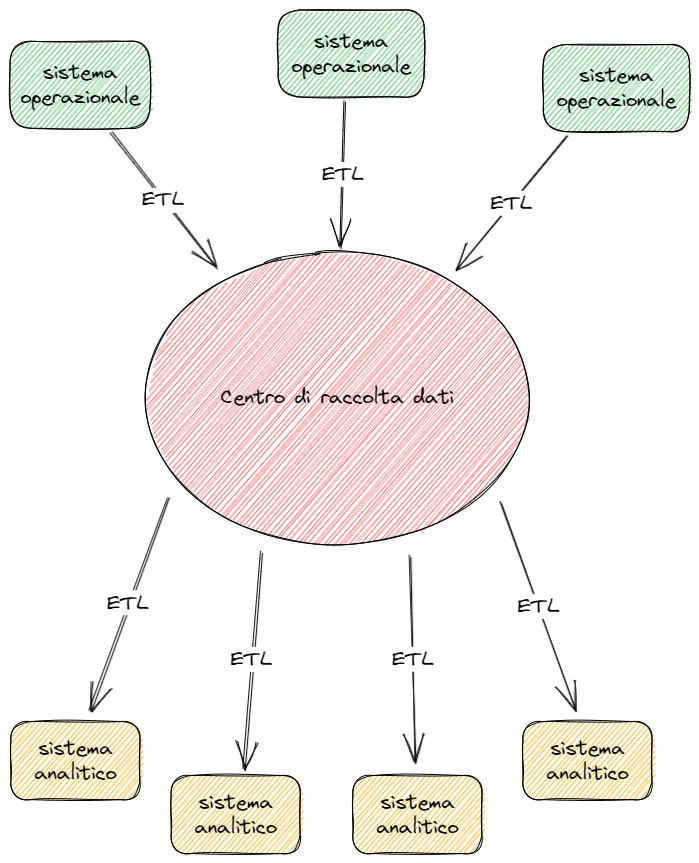
\includegraphics[scale = 0.4]{immagini/vista architetture centralizzate 2023-07-21 11.27.28.excalidraw.png}
\caption{rappresentazione ad alto livello di un architettura monolitica}
\label{fig:architettura monolitica}
\end{figure}

Il punto di raccolta dei dati viene storicamente realizzato utilizzando un data warehouse o un data lake. 
Il data warehouse è un modello di storage in cui i dati vengono raccolti dalle fonti e trasformati, per adattarsi a uno schema preciso. 
Questo permette poi di recuperarli utilizzando un approccio SQL-based. 
Sebbene l'utilizzo di uno schema unico renda piuttosto comoda la consultazione, esso rende complessa la trasformazione dei dati delle fonti.
Questi devono essere infatti trasformati in modo che sia possibile rappresentarli secondo lo schema del data warehouse.
All'aumentare del numero delle fonti aumenta la complessità e il costo di manutenzione del sistema e degli ETL in ingresso.
A livello organizzativo inoltre tende a creare figure professionali specializzate sullo schema e sulla tecnologia specifica del data warehouse. 
Queste persone diventano di fatto le uniche in grado di lavorare sul sistema, provocando un lock-in sui dipendenti e sulla tecnologia.
La situazione che si verifica in un data warehouse all'aumentare del numero di fonti viene paragonata da Zeghani in \cite{dehghani_data_2022} a quella descritta da Evans nei sistemi in cui si utilizza un unico modello per gestire un sistema che spazia su diversi domini.
Nel data lake invece i dati vengono salvati in forma grezza, estraendoli direttamente dai sistemi operazionali.
Vengono utilizzati processi ETL a monte del data lake, trasformando il dato grezzo in base al tipo di analisi che si vogliono effettuare su questo.
Il problema di questo approccio è che può diventare difficile individuare e capire il significato dei dati conservati nel data lake.
Al crescere della quantità e dell'eterogeneità dei dati conservati questa difficoltà tende ad aumentare.
In generale, le architetture monolitiche presentano un problema definito in \cite{perry_foundations_1992} come technical decomposition.
Con  technical decomposition si intende una divisione organizzativa in cui team diversi si occupano di svolgere compiti tra loro sequenziali e relativi allo stesso dominio.
Un esempio classico di questo approccio nell'ingegneria del software è il famoso modello a cascata, in cui la suddivisione dei vari passaggi (raccolta dei requisiti, specifiche, implementazione...) è assegnata a team diversi.

La criticità principale di questa suddivisione dei compiti è il costo associato al cambiamento in una qualsiasi delle componenti. 
Infatti, un cambiamento in qualsiasi punto del processo richiede procedure di sincronizzazione tra più team.
Con l'affermarsi dell'ideologia Agile \cite{fowler2001agile} e a seguito della corrente DevOps si è andati sempre più verso una suddivisione dei compiti basata sul dominio. 
Oltre al maggior costo di sincronizzazione, che porta a una maggiore resistenza al cambiamento, l'architettura monolitica mette una grande pressione sul ruolo dei data engineer.
Queste figure infatti devono essere in grado di interpretare i dati che provengono da diverse fonti e, allo stesso tempo, capire le esigenze dei data scientist, per trasformare i dati secondo i loro bisogni. 
Questo comporta un carico cognitivo importante per la figura professionale e spesso costituisce un collo di bottiglia nell'intero processo.
Un altro effetto collaterale di un'architettura monolitica è l'approccio dei team operazionali nei confronti dei propri dati.  
Tendenzialmente il team è infatti responsabile unicamente di garantire un servizio e i dati, estratti dal sistema dai data engineer, vengono trattati come prodotti collaterali. 
Ne consegue che le API che il team fornisce per raccogliere il dato vengano trascurate. 
Questo porta ad avere dati ``sporchi'' e delle API spesso naive e poco documentate.

\subsection{Domain ownership} \label{downership}
Il primo principio del Data Mesh cerca di applicare l'idea di separazione dei modelli esposta nel Domain Driven Design, per risolvere alcuni dei problemi associati alle architetture monolitiche.
In particolare si cerca di rendere il sistema scalabile, ridurre il carico dei data engineer e ridurre la technical decomposition.
Per risolvere questi problemi si cerca di spostare la responsabilità della gestione dei dati analitici da un'architettura centralizzata a una decentralizzata. 
La responsabilità sui dati viene quindi assegnata ai team che lavorano nei domini dove i dati vengono prodotti o utilizzati.
Questo approccio aumenta l'autonomia del dominio; infatti viene deciso internamente dal team che lavora sul dominio come rappresentare i dati.
Questo permette al sistema nel complesso di non essere influenzato dall'aumento dei sistemi che producono o utilizzano dati analitici, garantendo scalabilità.
In accordo con la legge di Conway, questo principio stravolge anche l'organizzazione dell'azienda.
Il team responsabile dei sistemi che lavorano su un dominio specifico diventa responsabile anche dei dati relativi a quel dominio.
Di conseguenza un cambiamento nel dominio, che si rispecchia in un cambiamento a livello di dati, influenza solo il team assegnato a quel dominio, diminuendo così la technical decomposition e la comunicazione fra team diversi.
Questo porta anche all'eliminazione del team di data engineer che viene distribuito su tutta l'azienda, favorendo anche il trasferimento delle nozioni ed eliminando il problema del carico cognitivo eccessivo che ricadeva su queste figure.
Questo tipo di gestione assicura inoltre che chi gestisce i dati abbia una buona conoscenza del dominio da cui questi provengono.
Ne consegue una maggiore comprensione del significato e del formato del dato che permette un migliore svolgimento delle operazioni di pulizia e presentazione dello stesso. 
I domini in cui i dati vengono prodotti vengono detti domini dei dati orientati alla fonte; questi hanno la responsabilità di fornire al resto dell'organizzazione i dati ricavabili dal sistema che gestiscono.
L'applicazione del DDD alla gestione dei dati porta anche alla formazione di nuovi domini, legati al mantenimento di un dato analitico ottenuto aggregando i dati analitici di alcuni domini orientati alla fonte.
Questo tipo di domino viene detto dominio dei dati aggregato.
Infine, i domini in cui i dati vengono trasformati, aggregati e utilizzati col fine di compiere analisi vengono detti domini dei dati orientati al consumatore. 
Anche in questo caso, dato che il team che aggrega e mantiene il dato è lo stesso che si occuperà di svolgere le analisi su questo, si garantisce che il dato abbia le caratteristiche necessarie per le analisi. 
Il grande problema di questo approccio è dato dall'aumento della complessità del sistema, che è inevitabile nei processi di decentralizzazione.
I restanti tre principi si occupano di stabilire come applicare a un sistema enterprise questo primo principio, che viene appunto definito come Domain Ownership.

\subsection{Data Product}
Il secondo principio prende il nome di Data Product (DP), e tratta le modalità con cui il dato analitico deve essere fornito.
L'obbiettivo è permettere l'applicazione del principio di Domain Ownership e facilitare il lavoro dei data scientist, che si stima passino più della metà del loro tempo nelle fasi di ricerca e di pulizia dei dati.
L'idea principale è di iniziare a considerare il dato come un prodotto, riprendendo le caratteristiche di un prodotto di successo definite in \cite{cagan_inspired_2017}. 
Un prodotto di successo dovrebbe essere non troppo costoso, di valore per il suo target e facilmente utilizzabile.
Con Data product si intende quindi un servizio o un insieme di servizi che si occupano della gestione di un dato analitico nella sua interezza, cercando di soddisfare chi deve usare quel dato.
Un Data product viene descritto come un Architectural Quantum \cite{ford_building_2022}, un componente di un'architettura implementabile indipendentemente che contenga tutti gli elementi che consentono il suo funzionamento in autonomia.
Questo comprende la gestione del codice, dei dati, dei meta-dati e l'applicazione delle politiche di gestione degli accessi e di rispetto della privacy.
Inoltre, per essere definito tale, una Data Product deve presentare le proprietà FAIR (Findable, Addressable, Interoperable e Reusable) definite in \cite{wilkinson_fair_2016}. 
Le proprietà FAIR nascono come insieme di principi che dovrebbero permettere a un'infrastruttura di supportare la condivisione, la scoperta e la ricerca di dati. 
Al fine di diminuire il tempo speso dagli scienziati per accedere al dato, il Data Product dovrebbe essere facilmente trovabile (findable).
Questo richiede che il Data Product possieda un identificativo univoco (URI) e condivida la documentazione sul dato, sulle modalità di accesso e sui suoi metadati.
Il Data Product dovrebbe inoltre fornire informazioni sul tipo di consumatori e di use case in cui è coinvolto. 
Il Data Product dovrebbe anche esporre le informazioni che permettano di capire le analisi possibili su quel tipo di dato e l'affidabilità dello stesso, in modo da permettere ai consumatori una valutazione consapevole sulle qualità e i limiti del dato.
Alcune informazioni che possono essere fornite per permettere questo sono la frequenza dei aggiornamento dei dati, la freschezza dei dati presentati e l'origine dei dati (lineage).
Al fine di poter garantire una continuità d'uso del Data Product deve garantire addressability, definita come la capacità di un sistema di essere raggiungibile in un unico modo, a prescindere dai cambiamenti.
Al fine di permettere l'aggregazione dei dati analitici presenti in diversi data product è necessario che questi siano fra loro interoperabili.
Per garantire l'interoperabilità in un Data Product vengono garantiti standard e armonizzazione sui punti di accesso e sul formato dei dati.
Bisogna inoltre essersi accordati su un sistema unico di tipi e su di un meccanismo di gestione dei polisemi, intesi come riferimenti alla stessa entità presenti in più contesti, e quindi modellati in maniera diversa.
Sarebbe ideale adottare uno schema uniforme per tutti i Data Product, in modo che sia possibile confrontare, riusare o comporre schemi partendo da quelli di altri Data Product.
Mentre il primo principio si concentra sul tenere il dato analitico nel dominio più adatto, lo scopo di questo secondo principio è garantire che il dato venga reso disponibile ad altri domini.
Proprio per questo, e per garantire il riuso, il Data Product dovrebbe essere facilmente interpretabile, e rendere quindi semplice la semantica del dato al di fuori del contesto in cui viene usato o in cui è stato creato.
Vene richiesto di progettare il Data Product in base ai possibili consumatori ma tenendo conto dell'impossibilità del prevedere gli utilizzatori e i requisiti futuri.
A livello organizzativo è prevista una nuova figura professionale, il Data Product owner, che avrà la responsabilità di garantire che un Data Product diventi un prodotto di successo.
Viene introdotta una figura apposita perché, come teorizzato anche da Evans parlando della collaborazione tra sistemi che utilizzano modelli diversi, è necessario avere una figura con un ruolo manageriale o di responsabilità per garantire che un team consideri la fornitura dati ad altri una priorità.



\subsection{Federated Computational Governance }\label{federated governance}
In un sistema che applica il Data Mesh rimangono da affrontare alcune tematiche relative alla governance.
In particolare, sarebbe desiderabile che la compliance, la privacy e le politiche di sicurezza siano garantite per tutti i Data Product. 
Inoltre, pur cercando di mantenere l'autonomia dei singoli domini, sono necessari meccanismi globali di interoperabilità per garantire che i Data Product non diventino database isolati e inutilizzabili.
Per garantire queste proprietà la proposta di Zeghani si articola su tre differenti aree: i processi per individuare le politiche di governance, la struttura organizzativa da adottare per garantire la governance e l'automatizzazione del tutto.
\subsubsection{System thinking applicato al Data Mesh}
Riprendendo l'assunzione di cambiamento continuo all'interno di una Data Mesh, l'enterprise viene considerato come un sistema in equilibrio.
Diventa necessario mantenere sia l'autonomia dei singoli domini, che permette di aumentare la produttività e la velocità di creazione dei Data Product, sia l'interoperabilità e la conformità con le politiche di governance, che garantiscono l'usabilità e il rispetto delle norme. 
Riprendendo il lavoro in \cite{meadows_thinking_2008} viene proposto di ragionare sul sistema utilizzando i concetti di leverage point e feedback loop.
Con il termine leverage point si intende un singolo elemento del sistema che, se modificato o inserito, può portare a grossi cambiamenti nel sistema complessivo.
I feedback loop invece sono strategie adottate per dare un ritorno costante su alcuni elementi del sistema, con lo scopo di incoraggiare o correggere alcune pratiche.
Il team di governance di una Data Mesh dovrebbe concentrarsi sull'individuazione dei leverage point, esprimibili come metriche misurabili nel sistema, e di utilizzare dei feedback loop per incoraggiare o segnalare ai singoli team come muoversi per migliorare rispetto alle metriche individuate. 

\subsubsection{Federated Governance}
Il termine Federated viene utilizzato per indicare, a livello organizzativo, la modalità con cui viene stabilita la governance all'interno dell'architettura.
Sono previsti due livelli di governance: quella locale e quella globale.
La governance locale viene gestita e applicata dai singoli Data Product.
Le politiche di governance locali si occupano di garantire che il dato fornito dal Data Product sia coerente e di qualità. 
La governance locale determina anche le modalità di conservazione, aggiornamento e rappresentazione del dato.
Queste responsabilità ricadono quindi sugli esperti del dominio che più si trova vicino al dato, in accordo con il principio di Domain Ownership.
Le politiche globali, invece, si occupano di garantire i requisiti di sicurezza, privacy e interoperabilità trasversalmente a tutti i domini. 
Il team che si occupa di governance viene composto coinvolgendo i responsabili di tutte le entità che devono applicare la governance e alcuni esperti con una conoscenza specifica dei requisiti che il sistema deve garantire nel complesso. 
Comprenderà quindi i responsabili di ogni Data Product (Data Product owner), il responsabile della self-serve-data platform, che verrà introdotta in seguito, delle figure professionali specializzate in privacy e sicurezza e dei facilitatori per la gestione della comunicazione fra le parti.
È compito di questo gruppo individuare i leverage point e i feedback loop necessari a tenere in equilibrio il sistema. 
A livello di interoperabilità, il team di governance dovrebbe definire un'interfaccia uniforme per la discoverability e l'accesso dei dati, delle convenzioni che definiscano un formato uniforme dei tipi e per l'individuazione e la rappresentazione uniforme dei polisemi.
A livello di privacy e sicurezza il team centralizzato dovrebbe concentrarsi sull'individuazione delle operazioni necessarie per i Data Product, indipendentemente dal dominio.

\subsubsection{Computational governance}
Con il principio di Computational governance si propone la possibilità di automatizzare il controllo delle politiche.
Viene teorizzato in \cite{dehghani_data_2022} che le scelte del team di governance siano espresse in forma di standard o di politiche automatizzabili.
Gli standard dovrebbero definire le regole sulle interfacce e sul formato dei dati. 
Questi standard dovrebbero essere implementati direttamente in componenti generiche, utilizzabili in ogni Data Product.
Vengono poi definite delle politiche per definire le modalità di accesso ai dati.
Il team di governance dovrebbe riflettere su come rendere implementabili queste politiche e creare un sistema uniforme per la definizione e l'applicazione di politiche a livello globale. 
Ogni politica dovrebbe essere quindi codificata, automatizzata e integrata nei Data Product; questo dovrebbe prevenire o rendere più difficili i processi di erosione e deriva all'interno dell'architettura.
Oltre all'applicazione della governance è necessario vengano automatizzati i processi di monitoraggio delle metriche individuate come leverage point del sistema.

\subsection{Self-Serve Data Platform}\label{self-serve data platform}
I principi di Data Product e Domain Ownership richiedono che i team analitici e operazionali introducano, oltre ai loro compiti primari, la responsabilità di condividere i dati su cui lavorano, rispettando metriche e requisiti abbastanza stringenti.
Per poter creare un sistema che scala all'aumentare del numero dei Data Product è inoltre necessario che quest'ultimi siano interoperabili; se i Data Product infatti non presentano un'interfaccia standard e un formato comune di trasmissione dei dati è necessario creare un'integrazione specifica per ognuno di essi. 
Senza un sistema di Data Product interoperabili diventa più complicato garantire al consumatore la possibilità di trovare, confrontare e utilizzare altri Data Product.
Rimangono poi le preoccupazioni riguardo alla governance.
Il principio di Federated Computational Governance si occupa di stabilire alcuni principi su come le politiche dovrebbero essere create e sulle caratteristiche queste che devono presentare.
Non viene però trattato come le politiche possano essere implementate e applicate da ogni Data Product, senza aumentare ulteriormente il carico di lavoro associato a ogni team.
Per finire, lavorare con i dati e con le politiche nel panorama tecnologico attuale richiede la conoscenza di tecnologie molto specifiche, e risulta difficile trovare figure professionali adatte da inserire in ogni team analitico od operazionale.
Per rispondere a queste perplessità Zeghani introduce il concetto di Self-Serve Data Platform.
La definizione che verrà utilizzata all'interno di questo lavoro di tesi per il termine ``piattaforma'' è la seguente: ``insieme di strumenti utilizzabili da team indipendenti per velocizzare lo sviluppo e ridurre il carico cognitivo''.
Si richiede quindi, per la costruzione di una Data Mesh, la creazione di una piattaforma che fornisca gli strumenti necessari per l'applicazione di tutti gli altri principi.
Lo scopo della piattaforma è facilitare il lavoro degli sviluppatori dei Data Product, creando strumenti per gestire operazioni agnostiche rispetto al domino.
Per diminuire il carico di lavoro e il carico cognitivo dei team uno degli obbiettivi della piattaforma è quindi la gestione del ciclo di vita del Data Product.
Con ciclo di vita si intende la creazione, la manutenzione e la modifica del prodotto.
L'obbiettivo è quindi rimuovere tutto il carico cognitivo legato all'utilizzo di tecnologie specifiche per la gestione dei dati e della privacy e creare degli strumenti, adatti per sviluppatori ``generalisti'', che consentano di concentrarsi sui problemi del dominio.
Il team che si occupa di un Data Product dovrebbe quindi occuparsi dei seguenti punti:
\begin{itemize}
    \item fornire le informazioni per la discoverability del prodotto (metadati),
    \item specificare le fonti, le modalità di aggiornamento e le trasformazioni da applicare ai dati per la costruzione e l'aggiornamento del Data Product,
    \item specificare le rappresentazioni e le modalità di accesso al dato ,
    \item specificare le politiche locali (gestione accessi, privacy, sicurezza) dei dati conservati.
\end{itemize}
La piattaforma, date queste informazioni, dovrebbe poi creare il Data Product e permettere al team responsabile di verificarne la correttezza e modificarlo. 
Le interfacce esposte da tutti i Data Product saranno quindi uguali, e questo permette di risolvere il problema del'interoperabilità.
Gli esperti di privacy e i data engineer lavoreranno per la realizzazione della piattaforma, rendendo gli strumenti messi a disposizione agli altri sviluppatori facilmente utilizzabili.
La piattaforma si occuperà anche della discoverability dei Data Product, creando e mettendo a disposizione un catalogo contenente i meda-dati che sono stati forniti da ogni Data Product.
Infine la piattaforma si occuperà di fare in modo che le politiche e le metriche proposte dal team centralizzato siano applicate e misurate su tutti i Data Product.
Nel lavoro di tesi si approfondirà l'utilizzo dell'architettura orientata ai servizi per la realizzazione di una Self-Serve Data Platform





\section{Architettura orientata ai servizi} \label{servizio}
In questo paragrafo viene approfondita l'architettura orientata ai servizi (abbreviata a SOA, Service Oriented Architecture).
Viene definita in \cite{josuttis_soa_2007} come architettura volta a gestire processi di business in sistemi distribuiti eterogenei e con nodi posseduti da diversi proprietari.
Dato che la definizione e gli elementi presentati non riguardano una soluzione specifica, in questo lavoro di tesi si considera SOA come uno stile architettonico.
Nei paragrafi successivi verranno trattati i requisiti impliciti che lo stile architettonico garantisce, alcuni vincoli opzionali e una possibile suddivisione dei servizi in categorie, proposta in \cite {josuttis_soa_2007}.

\subsection{Vincoli e proprietà SOA}
SOA nasce come architettura pensata per sistemi distribuiti complessi, inclusi i sistemi enterprise.
Definiamo con sistemi enterprise, riassumendo la definizione proposta in \cite{eneterpiseSysRood} come sistemi con le seguenti caratteristiche:
\begin{itemize}
    \item sono composti da persone, informazioni e tecnologie,
    \item effettuano operazioni di business,
    \item hanno un'organizzazione distribuita su più luoghi,
    \item forniscono specifici servizi e prodotti ai loro clienti.
\end{itemize}
I sistemi enterprise spaziano fra domini molto diversi, e questo richiede modelli diversi per la rappresentazione delle varie funzionalità che il sistema offre \ref{bounded context}.
Un'altra caratteristica dei sistemi enterprise è la tendenza del sistema a cambiare di continuo, rendendo la flessibilità uno delle proprietà critiche che il sistema dovrebbe garantire.
Si assume inoltre, come specificato dalla definizione, che ci possano essere più organizzazioni coinvolte, e che il sistema debba essere, per motivi geografici, amministrativi o tecnici, distribuito e con nodi eterogenei.
I vincoli imposti da SOA cercano di porre le basi di un sistema che possa, almeno parzialmente, risolvere requisiti specifici in un ambiente con le caratteristiche di qui sopra.
In primis viene introdotto il concetto di servizio, una componente software con descrizione esterna pensata per rendere esplicita una separazione dei modelli.
Un servizio dovrebbe fornire l'implementazione trasparente di una funzionalità del dominio.
Lo scopo della descrizione esterna è permettere l'utilizzo del servizio senza la necessità di conoscere i dettagli implementativi.
Allo stesso modo se il servizio soddisfa in maniera trasparente una funzionalità presente nel dominio è più intuitivo l'utilizzo e ne permette una maggiore facilità di utilizzo anche fra organizzazioni diverse.  
Avere dei servizi che comunicano utilizzando unicamente la conoscenza delle rispettive interfacce permette una bassa inter-dipendenza a livello di codice.
Questo consente al servizio di cambiare implementazione mantenendo fissa l'interfaccia, diminuendo così la resistenza al cambiamento del sistema.
Avere come unico vincolo l'interfaccia permette anche di lavorare con nodi e team eterogenei, che presentano caratteristiche ed esigenze di lavoro/strumenti di sviluppo diversi.
Un'altra proprietà necessaria per permettere la crescita del sistema è garantire l'interoperabilità dei servizi; ottenere dei servizi interoperabili permette di comporli, garantendo riuso e velocizzando il processo di sviluppo e l'introduzione di nuove funzionalità. 
Il vincolo essenziale che propone una SOA è quindi una suddivisione delle diverse funzionalità di dominio in entità, tra loro il più possibile indipendenti, che espongono un'interfaccia indipendente dall'implementazione, linguaggio o ambiente di sviluppo. 

\subsection{Elementi opzionali} 
È possibile introdurre ulteriori vincoli, che aumentando un po' la complessità garantiscono alcune proprietà aggiuntive 
\subsubsection{Contratto}
Per diminuire l'ambiguità sulle responsabilità dei servizi, in aggiunta all'interfaccia è possibile introdurre un contratto.
Un contratto facilita l'utilizzo e fornisce maggiori garanzie al fornitore e all'utilizzatore.
Si occupa di specificare i requisiti e i limiti di utilizzo del servizio e fornisce alcune garanzie sulle operazioni e sui risultati forniti.
Per garantire l'interoperabilità nell'architettura è necessario che il contratto di ogni servizio sia noto, comprensibile a entrambe le parti e privo di ambiguità.
È possibile applicare le idee introdotte col Design by contract \cite{meyer1992applying} per automatizzare, almeno parzialmente, il controllo sulle responsabilità delle due parti. 
Questo rende più difficile l'erosione e la deriva per quanto riguarda il rispetto del contratto. 
\subsubsection{Enterprise Service Bus}
Al crescere del numero dei servizi e dell'ampiezza del sistema (in termini di entità coinvolte) diventa difficile imporre la stessa interfaccia a tutti i servizi.
Diventa quindi necessario per ogni servizio occuparsi dell'integrazione con gli altri servizi con cui collabora o che lo compongono.
Per far fronte a questi problemi viene introdotto il concetto di enterprise Service Bus, abbreviato in ESB. 
Possiamo considerare un ESB come un mezzo di trasmissione centralizzato, utilizzato per recapitare informazioni ai servizi. 
In base a come viene strutturato, consente di garantire alcune proprietà sul messaggio.
La sua presenza garantisce l'accesso ai servizi in maniera trasparente rispetto all'interfaccia specifica del servizio e si occupa di esporre tutti i servizi e di gestire la conversione dei tipi all'interno dell'architettura. 
Ogni servizio dovrà quindi occuparsi dell'integrazione con l'ESB, che a sua volta garantirà a la comunicazione fra servizi eterogenei.
Un ESB può essere utilizzato anche per controllare parti del contratto fra le componenti e applicare politiche di sicurezza/autenticazione sui messaggi.
Infine un ESB può attuare politiche di routing per garantire trasparenza di accesso. 
È possibile associare a ogni servizio un nome logico, e dato questo chiedere all'ESB
di raggiungere l'indirizzo fisico corrispondente.
Questo permette a un servizio di cambiare indirizzo o di essere replicato senza che gli utilizzatori debbano esserne a conoscenza. 
Al crescere dell'enterprise è possibile anche un architettura con più ESB, ognuno dei quali deve essere integrato con gli altri. 
Questo può essere necessario per motivi di retro-compatibilità, in seguito all'unione di più sistemi o perché gli ESB vengono utilizzati per fornire garanzie diverse.

\subsubsection{Servizi applicativi}\label{servizi applicativi}
La suddivisione delle funzionalità in servizi che rispecchiano le funzionalità del domino permette di tenere il dominio al centro, in accordo con quanto detto nel paragrafo \ref{DDD}. 
I problemi di questo approccio sono il rischio di isolamento del codice prodotto dal team rispetto alla codebase e il rischio di incoerenza fra i prodotti portati.
Inoltre questo può portare alla duplicazione di alcune operazioni, che sono simili anche se svolte in domini differenti.
Per risolvere questo problema è possibile introdurre il concetto di servizi applicativi (definiti così in \cite{erl_service-oriented}): dei servizi che non implementano una funzionalità del domino ma che svolgono delle operazioni generiche.
Si crea quindi un'architettura a più strati (Multi-layer architecture), dove i servizi applicativi vengono utilizzati dai servizi standard per garantire uniformità sullo svolgimento di alcune operazioni, per velocizzare lo sviluppo e per garantire riuso.
Un problema di questo approccio è che da questi servizi potrebbero dipenderne molti altri, rendendo quindi i servizi applicativi molto difficili da modificare o sostituire.
Potrebbe inoltre risultare particolarmente critica la fase di progettazione e sviluppo, in quanto queste componenti verranno integrate in domini e in situazioni molto diverse.
L'introduzione dei servizi applicativi è un tentativo di mediare le due principali metodologie di divisione del lavoro secondo \cite{richards_fundamentals_2020}: decomposizione tecnica (già accennata nel paragrafo \ref{architetture monolitiche}), in cui il sistema viene diviso sulla base del tipo di operazione e decomposizione sulla base del modello del domino, presentata nel paragrafo \ref{bounded context}.

\subsection{Categorie di servizi}
Data l'ampiezza del concetto di servizio, per semplificare la creazione delle architettura è possibile dividere i servizi in categorie, ognuna delle quali presenta vincoli specifici.
Nell'ottica di fornire dei vincoli più stringenti con lo scopo di fornire proprietà aggiuntive all'architettura, in letteratura sono presentate alcune proposte di categorizzazione di servizi. 
In questo lavoro di tesi viene considerata, come esempio di questo approccio, quella riportata in \cite {erl_service-oriented}.
Viene presentata un'architettura a più strati, in cui i servizi di ogni strato possono essere costruiti utilizzando servizi degli strati inferiori.
Vengono individuate le tre tipologie di servizi in base al loro rapporto col backend, dove con il termine backend viene definito un sistema non esposto all'utente necessario per soddisfare le richieste; spesso si tratta di sistemi che memorizzano dati.
Si procede ora analizzando le tipologie di servizi presentate da questa architettura.
\subsubsection{Servizi di base}
Vengono definiti come servizi di base i servizi che implementano funzionalità semplici, che modellano la logica del dominio o rendono trasparente il backend garantendone un accesso orientato al dominio.
Non vengono fatte distinzioni sul tipo di operazioni che i servizi possono effettuare; è possibile quindi che questi effettuino sia scritture che letture sul sistema di backend.
Per appartenere a questa categoria un servizio deve essere stateless, mediare l'accesso al backend in maniera trasparente e sicura e non utilizzare o dipendere da altri servizi.
Un'architettura con solo i servizi di base viene definita fundamental SOA.  
\subsubsection{Servizi composti }
I servizi composti sono servizi creati componendo più servizi di base o altri servizi composti, sono stateless, e con tempo di esecuzione limitato. 
Si occupano principalmente di comporre servizi di base con lo scopo di mantenere la coerenza in più sistemi di backend, che potrebbero presentare elementi ridondanti che necessitano una sincronizzazione.
Al fine di garantire la coerenza nel sistema,è compito di questi servizi  assicurarsi che le proprietà ACID vengano mantenute in tutti i sistemi di backend coinvolti.
Quindi viene introdotto il concetto di servizi composti per rendere trasparenti quei servizi che per garantire alcune funzionalità coinvolgono più sistemi di backend.
Un'architettura che comprende servizi di base e servizi composti viene detta federated SOA.
\subsubsection{Servizi di processo}
I servizi di processo si occupano di soddisfare le richieste che necessitano che il sistema consideri il concetto di sessione.
Possono inoltre essere collegati a più sistemi di frontend e soddisfano una richiesta dell'utente finale.
I servizi di processo possono essere composti dai servizi presenti nei due strati sottostanti e si occupano di mantenere lo stato di una sessione.
Si distinguono dai servizi compositi per la gestione dell'interazione con l'utente e dei problemi derivanti dalla gestione dello stato.
Possono fare in modo che lo stato venga conservato nel backend per garantire una continuità del servizio su più sessioni. 
Un'architettura che comprende servizi di processo viene definita process-enabled SOA. 

\subsubsection{Altre categorie}
Sono presenti altre categorie proposte in letteratura per definire alcune proprietà di specifiche tipologie di servizi, ed è possibile categorizzare i servizi in base all'architettura che si sta realizzando. 
Alcuni esempi sono la categorizzazione in base alle operazioni sul backend. 
Dato che i servizi che lavorano in lettura e i servizi che lavorano in scrittura necessitano di requisiti molto diversi, è possibile raggrupparli in queste due categorie.
Un'altra possibile categorizzazione riguarda i diversi consumatori del servizio. 
I requisiti di un servizio possono infatti dipendere dai consumatori; si propone quindi di utilizzare questo criterio per classificare servizi. 
Un esempio di questo approccio è la classificazione di servizi in servizi pubblici e  servizi interni all'enterprise.

\chapter{Architettura software}\label{architetturaLogica}
In questo capitolo viene spiegato come è stata costruita l'architettura, il razionale dietro alle scelte e alle caratteristiche del sistema proposto. 
Nel primo paragrafo saranno approfondite le motivazioni che hanno portato alla realizzazione di questa architettura software.
In seguito si procederà con un'analisi degli agenti, termine utilizzato per indicare le entità che dovranno interagire con il sistema che si propone di realizzare.
Dagli agenti verranno ricavati gli use-case, le operazioni che gli agenti vorrebbero poter effettuare per soddisfare i propri bisogni.
Dalle operazioni e dal contesto in cui queste devono essere effettuate verranno ricavati i requisiti.
Verranno quindi presentate in maniera graduale le componenti ritenute necessarie per la realizzazione di un'architettura che soddisfi i requisiti individuati. 
Si cercherà di spiegare le caratteristiche e le motivazioni dietro a ogni componente individuata.
Infine nell'ultimo paragrafo verrà confrontata l'architettura proposta confrontandola con le architetture proposte per la creazione di una Data Mesh presenti in letteratura.

\section{Motivazioni per la costruzione dell'architettura}
In \cite{whoneedsanArchitect} si cerca di ricavare una definizione operativa per il termine ``architettura software''. 
Nel lavoro, un'architettura software viene considerata come l'insieme delle scelte che, se prese correttamente a inizio progetto, facilitano la riuscita dello stesso.
Si ritiene quindi che lo scopo dell'architettura sia di definire inizialmente l'insieme delle scelte che se cambiate in seguito potrebbero compromettere la costruzione del sistema.
Parafrasando si definisce un'architettura software come l'insieme delle scelte irreversibili che coinvolgono la progettazione del sistema.
Alcuni principi dell'ideologia Agile riportati in \cite{martin_fowler_xp_2002} e ripresi in \cite{whoneedsanArchitect} affermano però che la complessità di un sistema software è proporzionale al numero di elementi immutabili che lo compongono.
Nell'articolo si argomenta poi che, contrariamente ad altri tipi di architetture, i sistemi software non presentano elementi intrinsecamente immutabili. 
Seguendo questa linea di pensiero, gli unici elementi immutabili del sistema sono quelli definiti dall'architettura.
Si può quindi affermare che rimuovere l'architettura rimuove la presenza di elementi immutabili in fase di progettazione e quindi riduce la complessità del sistema.
Prendendo spunto da questa osservazione, si vuole proporre un'architettura utilizzabile come strumento per facilitare il cambiamento, non per renderlo più complesso. 
In \cite{designChoiche} viene individuato come problema principale per l'evoluzione di un'architettura la così detta ``knowledge vaporization'', intesa come la mancanza nella documentazione dei motivi che hanno portato a una specifica modifica del sistema. 
Questo può portare a non rispettare una scelta compiuta in precedenza. 
La mancanza di documentazione, infatti, può portare a ignorare la scelta presa in passato, o a considerarla sbagliata perché se ne ignorano i motivi.  
L'altra possibilità è che, sempre a causa della mancata comprensione delle motivazioni dietro a scelte passate, queste vengano ritenute giuste, anche nel caso in cui sia cambiato il contesto che le ha determinate.
Quest'ultima situazione porta a una paralisi del sistema, rendendone difficile l'evoluzione.
Un sistema non pienamente compreso può quindi perdere la sua integrità strutturale o diventare di fatto irreversibile.
Si ritiene quindi che sia necessaria un'architettura, vista non come una guida alla realizzazione del sistema, ma come una proposta pensata per essere modificata. 
L'architettura dovrebbe documentare le proprietà che il sistema dovrebbe garantire, i motivi per cui sono ritenute importanti e i vincoli che si ritengono necessari per garantirle.
Dal punto di vista dell'architettura quindi l'obbiettivo della tesi è creare una proposta che non ha la presunzione di risolvere un problema, ma che cerca di porre le basi a livello accademico per un dialogo sul tema. 
Fornire un razionale ben documentato dovrebbe permettere di discutere un'architettura e di capire, al modificarsi dei requisiti, del contesto o della comprensione del problema, in che modo sia necessario cambiarla.
Si considera quindi l'architettura come uno strumento dinamico da mettere continuamente in discussione, e che permetta agli sviluppatori di orientarsi su cosa andrebbe e non andrebbe fatto, ma soprattutto sulle motivazioni dietro alle scelte.
L'architettura proposta viene creata pensando a un'azienda enterprise che vuole provare ad applicare i principi del Data Mesh.
Si è scelto di lavorare sul Data Mesh perché, pur essendo un trend largamente adottato nelle aziende enterprise, viene spesso utilizzato come buzzword; inoltre scarseggiano i lavori sul tema in ambito accademico \cite{goedegebuure2023data}.
In particolare, si cercano di affrontare alcune delle perplessità principali sollevate dall'idea di Data Mesh.
La creazione di Data Product indipendenti rischia di incentivare la frammentazione dell'architettura, andando a impattare sull'interoperabilità e sulla coerenza della stessa.
L'altro tema importante è il riuso, dato che una divisione a livello di dominio sulla gestione dei dati porta a inevitabili duplicazioni all'interno dei Data Product.
Questo lavoro vuole quindi iniziare a esplorare la progettazione della Self-Serve Data Platform, componente pensata per fornire gli strumenti necessari per la realizzazione dei Data Product, minimizzando lo sforzo per la loro creazione e garantendo riuso e uniformità.
In \cite{zachman1987framework} Zachman afferma che la decentralizzazione di un sistema senza una struttura porta al caos. 
Si cerca quindi di definire una struttura che renda efficace in un sistema enterprise la decentralizzazione della responsabilità dei dati proposta dai principi di Data Mesh.

Si adotta lo stile di architettura orientata ai servizi perché il contesto in cui viene applicato il data Mesh presenta le stesse sfide che hanno portato all'introduzione della SOA. 
Il secondo motivo è che, essendo il concetto di servizio abbastanza generico, è garantito un certo margine di flessibilità nella costruzione dell'architettura.
Inoltre, essendo il concetto ben radicato nell'ingegneria del software, l'utilizzo di servizi permette di utilizzare terminologie e classificazioni delle componenti ben chiare alla comunità, facilitando così la comunicazione.
Si cercherà quindi di replicare l'idea di architettura a strati, con l'obbiettivo di fornire componenti utilizzabili in tutti i Data Product.

\section{Requisiti dell'architettura}\label{requisiti}
In \cite{brooks_no_1987} Brooks parla dei requisiti in questi termini: ``The hardest single part of building a software system is deciding precisely what to build''. 
La necessità di un'analisi approfondita dei requisiti è fondamentale nella realizzazione di un sistema software; un sistema software elegante e ben costruito non è di nessuna utilità se risolve il problema sbagliato \cite{pressman2005software}.
Il processo di raccolta dei requisiti risulta facilitato in questo lavoro di tesi per tre motivi:
\begin{itemize}
    \item il sistema che si vuole definire è astratto e si basa su principi ben definiti,
    \item non è presente un committente umano con cui interagire, non è quindi necessaria la fase di comunicazione per estrarre la sua idea di architettura e applicarla al sistema,
    \item parte delle analisi proposte sono state affrontate e discusse nei vari articoli sul Data Mesh.
\end{itemize}
Si è comunque svolta l'analisi dei requisiti, con lo scopo di rendere espliciti i motivi per cui sono stati individuati i requisiti poi utilizzati per la costruzione dell'architettura.
Inoltre, ri-prendere il problema ripartendo dai requisiti ha permesso di arrivare a conclusioni che in alcuni punti differiscono rispetto a quelle presentate in letteratura.
Per individuare e definire i requisiti del sistema si è deciso di adottare la tecnica degli Use Case, integrandola con quanto riportato in \cite{dehghani_data_2022}.
Prima di procedere però con gli Use Case viene consigliato in \cite{cockburn2008writing} di definire lo scopo principale del sistema.
L'architettura che si propone vuole supportare i team di un  sistema Enterprise nell'applicazione dei principi di Data Mesh. 
Questo significa realizzare e fornire strumenti utili a ogni team, a prescindere dal dominio in cui questi lavorano.
Si assume che l'enterprise sia soggetto a continui cambiamenti, che condizionano anche la gestione dei dati analitici. 
Si desidera che l'architettura permetta, in maniera scalabile, di effettuare le seguenti operazioni:
\begin{itemize}
    \item aggiunta di nuove fonti da cui estrarre dati,
    \item aggiunta di nuove analisi da effettuare sui dati,
    \item modifiche delle analisi o dei dati conservati.
\end{itemize}

\subsection{Use Case}
La tecnica degli Use Case prevede l'elaborazione e la documentazione dei requisiti tramite l'impersonificazione degli utilizzatori del sistema e l'analisi delle loro interazioni con esso. 
Il primo passo per la creazione di Use Case è l'individuazione degli agenti principali che interagiscono col sistema.
Gli agenti sono una rappresentazione astratta di tutti gli utenti del sistema, raggruppati in base alle loro caratteristiche e ai loro obbiettivi. 
Per ogni agente si è cercato di individuare il motivo che lo spinge a utilizzare sistema che si vuole realizzare e le operazioni che il sistema gli dovrà permettere di effettuare. 
Gli agenti principali individuati in una Data Mesh sono i seguenti: team operazionale, team analitico, Data Product Owner e team di governance.
L'altro gruppo coinvolto sarebbe il team responsabile della Self-Serve Data Platform.
Il team però non viene considerato negli Use Case perché che si occuperà della realizzazione del sistema non del suo utilizzo. 
A eccezione del Data Product Owner si è deciso di considerare come agenti i team di lavoro.
Risulta infatti comodo in questa situazione specifica considerare i team nel loro insieme per individuare gli obbiettivi e le operazioni necessarie. 
La suddivisione interna al team e gli eventuali obbiettivi individuali non verranno quindi considerati.

\subsubsection{Team operazionale}
I team operazionali sono i team che si occupano di realizzare e mantenere le funzionalità offerte dal sistema enterprise.
L'obbiettivo dei team operazionali è di garantire che il sistema enterprise fornisca all'utente le funzionalità previste. 
Il principio di Domain's Ownership, introdotto con il Data Mesh, aggiunge però a questi team la responsabilità di fornire i dati su cui lavorano al resto dell'enterprise.
Per soddisfare questa responsabilità si chiede al team di creare e mantenere un Data Product.
La routine di creazione di un Data Product partendo dai dati del team operazionale prevede diversi passaggi.
In primo luogo è necessario che il team individui fra i dati su cui lavora quelli di interesse per l'enterprise.
Questa operazione mette a rischio l'autonomia del team ed è una delle possibili criticità dei principi del Data Mesh. 
Far lavorare il team operazionale sui dati estratti dal loro sistema permette di avere persone che lavorano su dati che comprendono. 
Il problema è che per capire a quale parte dei dati è interessato il resto dell'enterprise è necessaria una conoscenza che va al di fuori del dominio applicativo. 
Una possibile soluzione è mettere in contatto il team operazionale con i team analitici, ma così facendo si creano comunicazioni inter-team che limitano la scalabilità del sistema all'aumentare di fonti e consumatori.
Un compromesso può essere lasciare carta bianca al team operazionale che dovrà cercare di fare in modo che le informazioni siano le più utili possibili, basandosi unicamente sulla conoscenza locale del dato.
Una volta definiti i dati da fornire al resto dell'enterprise, è necessario effettuare un operazione di ETL, per spostare il dato dal database operazionale a un database usato per le analisi. 
Questo viene ritenuto necessario per i seguenti motivi:
\begin{itemize}
    \item mantenere il dato nel database operazionale aumenta il carico di lavoro di un sistema che ha come scopo principale di fornire un servizio all'utente;
    \item le operazioni di trasformazione e pulizia dei dati, da effettuare per presentare dei dati adatti alle analisi, andrebbero applicate a ogni richiesta; 
    questo porterebbe a un grosso costo computazionale aggiuntivo, evitabile applicando le trasformazioni una volta sola e salvando i dati in un altro punto;
    \item dividendo il database analitico e quello operazionale è possibile organizzare il database analitico in maniera più consona in base al tipo di richieste, che potrebbero essere diverse da quelle effettuate sul database operazionale.
\end{itemize}
Il team operazionale dovrà poi creare un'interfaccia per fornire l'accesso ai dati al resto dell'enterprise.
Per motivi di sicurezza e riservatezza si ritiene necessario che l'accesso a questi dati sia mediato, evitando quindi di esporre direttamente l'accesso al database analitico.
Infine, il team operazionale deve poter modificare e aggiornare il dato analitico conservato.
Questa serie di operazioni comporta un carico di lavoro aggiuntivo non indifferente per il team operazionale. 
Si elencano qua sotto, partendo dai passaggi necessari per la creazione del Data Product, quali operazioni si ritiene debbano essere facilitate dall'architettura.
Il requisito fondamentale su cui si basa la progettazione della piattaforma è semplificare il più possibile la creazione e la manutenzione del Data Product.
L'individuazione e la selezione dei dati da presentare, sebbene sia una fase interessante e potenzialmente problematica del processo non è stata considerata come requisito per l'architettura. 
Questo perché si tratta di un compito difficilmente automatizzabile e di natura più organizzativa che tecnica.
È possibile invece aggiungere tra i requisiti il supporto per tutte le operazioni di ETL: estrazione, trasformazione e salvataggio dei dati.
Per il salvataggio dei dati è auspicabile che venga semplificata l'integrazione con un database analitico. 
Sarebbe preferibile che il team operazionale non debba imparare a utilizzare una tecnologia specifica per salvare i dati analitici, in modo da ridurre il carico cognitivo.
Si richiedono poi degli strumenti per mettere il team operazionale nelle condizioni di pulire e trasformare il dato.
Infine, si richiede il supporto per la fase di estrazione, in particolare si vuole garantire che le modifiche del database operazionale vengano riportate, con frequenza di aggiornamento variabile, anche nel database analitico.
Data la necessità di esporre il dato al resto dell'architettura, si individua come ulteriore requisito la creazione di un'interfaccia comune a tutti i Data Product.
Questo garantisce, oltre alla riduzione del carico di lavoro, la standardizzazione delle interfacce dei Data Product.
La presenza di interfacce standard facilita inoltre la creazione di strumenti utilizzabili in ogni Data Product.

\subsubsection{Team analitico}
Il team analitico ha come scopo principale la realizzazione di analisi sui dati dell'enterprise.
Dato che l'obbiettivo del Data Mesh è permettere di estrarre valore partendo dati, è fondamentale che l'architettura faciliti il lavoro del team analitico.
In particolare i compiti del team analitico sono l'individuazione dei dati di interesse, la realizzazione del sistema di analisi e la presentazione dei risultati. 
Uno degli obbiettivi dei principi del Data Mesh è la velocizzazione della ricerca di dati analitici, che rischia altrimenti di  diventare problematica al crescere del numero di fonti. 
Si stima infatti che una buona parte del tempo di lavoro del team analitico sia impiegata nella ricerca, comprensione e pulizia di dati analitici.
Per mitigare il problema il Data Mesh propone che ogni Data Product presenti delle informazioni che raccontino le proprietà del dato conservato.
Queste informazioni dovrebbero permettere al team analitico di capire se il dato è utilizzabile per effettuare le analisi che il team si prefigge. 
Il team analitico quindi utilizzerà queste informazioni per individuare i dati di interesse. 
Una volta trovati i dati il team analitico farà richiesta al Data Product per poterli ottenere.
Una volta ottenuti i dati spetta al team analitico trasformarli, aggregarli e filtrarli in base alle analisi da effettuare.
Infine il principio di Domain Ownership richiede al team analitico di mantenere e condividere questi dati, insieme ai risultati ottenuti, con il resto dell'enterprise, andando a creare un'altro Data Product.
Questo consente di replicare gli esperimenti e di utilizzare i risultati ottenuti dal team per effettuare nuove analisi.
Le analisi svolte dal team analitico auspicabilmente permetteranno di compiere delle scelte sulla base di quanto osservato nei dati, rendendoli di fatto un asset di valore per l'organizzazione.
Si elencano qui sotto le operazioni, svolte dal team analitico, che si ritiene debbano essere facilitate dall'architettura.
Prima di tutto l'architettura dovrebbe fornire un servizio per facilitare la ricerca dei dati analitici, sfruttando le informazioni presenti nei Data Product.
Considerando quindi le necessità del team analitico, viene aggiunto ai requisiti dell'architettura un supporto alla presentazione dei dati che descrivono il Data Product. 
Questo richiede quindi che tutti i team siano in grado di condividere, con sforzo minimo, i dati relativi al proprio Data Product, e che questi dati siano facilmente consultabili dal resto dell'enterprise.
È inoltre richiesto che il team analitico sia sempre in possesso delle informazioni necessarie per effettuare richieste ai Data Product, e che queste informazioni vengano aggiornate nel caso di modifiche ai Data Product coinvolti.
Come per il team operazionale poi, sono richiesti servizi per facilitare la creazione del Data Product. 
Una differenza rispetto a quanto descritto per il team operazionale riguarda la procedura di ETL, che coinvolgerà altri Data Product e non un database operazionale.
Questo richiede che venga esteso il supporto all'aggiornamento del Data Product anche quando le fonti sono altri Data Product. 
Inoltre il sistema di estrazione e pulizia deve poter facilitare l'aggregazione di dati mantenuti da più Data Product differenti e quindi potenzialmente con formati e rappresentazioni differenti.
Riassumendo, vengono individuati questi nuovi requisiti per l'architettura: 
\begin{itemize}
    \item supporto alla ricerca dei dati, utilizzando quanto fornito dai Data Product,
    \item strumenti che facilitino ai Data Product la condivisione delle informazioni sui dati conservati,
    \item strumenti che mantengano le informazioni necessarie per contattare un Data Product,
    \item estensione del supporto per l'aggiornamento, che dovrà permettere di lavorare anche coi Data Product,
    \item estensione del supporto per la trasformazione, che dovrà permettere  di aggregare i dati da diverse fonti.
\end{itemize}

\subsubsection{Data Product owner}
Il Data Product owner è una figura professionale introdotta dal Data Mesh.
Viene assegnato un Data Product owner a ogni Data Product; questo attore ha la responsabilità di assicurare che il Data Product realizzato e mantenuto rimanga una risorsa di valore per l'organizzazione. 
Il principio di Domain's Ownership richiede che la responsabilità sui dati analitici venga decentralizzata; il Data Product owner è la figura su cui ricade questa responsabilità.
A livello organizzativo avere una figura con potere decisionale che sia responsabile del Data Product assicura che questa responsabilità non venga trascurata.
In assenza di una figura di questo tipo infatti i team potrebbero considerare queste pratiche come secondarie.
Si è deciso di inserire uno Use Case dedicato al Data Product owner per sottolineare gli obbiettivi e le operazioni comuni nei team analitici e operazionale volte a garantire la qualità di un Data Product.
Per assicurare che il dato analitico sia di valore è necessario che le fasi di pulizia e trasformazioni siano state progettate ed  effettuate meticolosamente.
Una metrica per misurare il valore di un  Data Product è il numero di ``consumatori'' del prodotto.
Per aumentare l'appetibilità del Data Product il Data Product owner dovrà assicurarsi che la descrizione fornita dal DP sia chiara e che il dato conservato sia di interesse. 
La descrizione dovrebbe comprendere una spiegazione ad alto livello del dato conservato, facendo in modo che sia comprensibile anche a chi non conosce il dominio di provenienza dei dati.
Poi è necessario vengano spiegate, in maniera completa e non ambigua, le modalità con cui il dato è stato realizzato, in modo che sia possibile capire come utilizzarlo.
Infine dovrebbero essere rese esplicite alcune metriche sulla qualità del dato, e alcune informazioni sulla freschezza e sulla frequenza con cui questo viene aggiornato.
Infine è compito del Data Product owner assicurarsi che le informazioni conservate rispettino i vincoli di riservatezza e confidenzialità.
Questo deve essere garantito in due contesti:
\begin{itemize}
    \item le informazioni e le metriche con cui viene presentato il dato non devono contenere informazione sensibili o permettere di risalire a esse,
    \item si deve fare in modo che durante l'accesso al dato analitico le informazioni riservate vengano inviate solo a chi ne ha diritto.
\end{itemize}
Infine, il Data Product owner deve poter ottenere un feedback sull'interesse che il suo prodotto riscuote a livello di enterprise, e deve poterlo modificare di conseguenza.
Molti dei compiti e delle responsabilità del Data Product owner coinvolgono comunicazione, pianificazione e organizzazione interna al team, e sebbene molto interessanti non verranno approfonditi in questa tesi.
Dal punto di vista tecnico sono invece stati individuati alcuni requisiti aggiuntivi, ritenuti necessari per permettere al Data Product owner di effettuare il suo lavoro.
Per garantire che venga rispettata la confidenzialità di alcuni dati é necessario che sia presente un sistema di autenticazione.
Si ritiene che il sistema debba essere gestito centralmente e utilizzato da tutti i Data Product all'interno dell'enterprise, per evitare la realizzazione e manutenzione di tanti sistemi diversi. 
Il Data Product owner dovrebbe essere poi messo nelle condizioni di definire delle politiche che restringano l'accesso ai dati sulla base dei ruoli degli utenti che effettuano la richiesta.
È quindi necessario fornire uno strumento per la codifica e l'applicazione automatica delle politiche.
Altri strumenti che possono essere forniti riguardano l'applicazione automatica di tecniche di privacy. 
In particolare  viene proposto in \cite{dehghani_data_2022} di fornire supporto per l'applicazione di tecniche di anonimizzazione, da applicare ai dati conservati, e tecniche di differential privacy \cite{dwork2006differential}, da applicare alle metriche fornite sul Data Product.
Per garantire al Data Product owner la possibilità di ottenere un riscontro sul successo sul Data Product è possibile aggiungere ai requisiti la possibilità a livello di organizzazione di recensire un Data Product. 
Si potrebbe inoltre fornire uno strumento di analisi, da integrare in ogni Data Product, che monitori il numero e il tipo di richieste effettuate.

\subsubsection{Team di governance}
Il team di Governance, che come già riportato nel Paragrafo \ref{federated governance}, dovrebbe occuparsi di garantire l'uniformità e imporre il rispetto di alcune politiche globali a tutti i Data Product. 
Le attività individuate per il team di governance sono le seguenti:
\begin{itemize}
    \item stabilire quali sono i polisemi e come gestirli,
    \item stabilire le interfacce e i formati standard, comuni all'architettura,
    \item stabilire alcune politiche comuni, da applicare a ogni Data Product,
    \item monitorare la conformità dei diversi Data Product alle direttive di governance.
\end{itemize}
Il team interagirà con il sistema in maniera marginale. 
Avrà un ruolo molto importante invece in fase di progettazione.
Dalle attività individuate però è possible ricavare alcuni requisiti per l'architettura.
Un'interfaccia standard per i Data Product è stata già aggiunta ai requisiti per facilitare il lavoro dei team operazionali e analitici.
Per la definizione e l'applicazione automatica di politiche globali è necessario rivedere il requisito sull'applicazione delle politiche discusso nel paragrafo sul Data Product owner.
Oltre all'applicazione delle politiche locali deve infatti tenere conto e applicare le politiche globali, definite dal team di governance. 
Si vuole quindi un sistema che permetta, una volta dichiarate le politiche globali, di applicarle alle richieste di ogni Data Product.
Per garantire il monitoraggio della conformità delle politiche di governance viene proposto di inserire nell'interfaccia del Data Product una serie di operazioni riservate al team di governance.
In particolare, oltre al monitoraggio sarebbe opportuno garantire al team di governance la possibilità di modificare le politiche locali o i dati forniti dal Data Product, permettendo così di intervenire tempestivamente in caso le violazioni abbiano un impatto in ambito legale.
\subsection{Sintesi dei requisiti}
I requisiti sono rappresentati nella Figura\ref{fig:requisitiBusiness} e nella Tabella \ref{tab:requisitiTec}. 
In particolare nella Figura \ref{fig:requisitiBusiness} sono stati inseriti i requisiti a livello di business, con lo scopo di mostrare le esigenze ad alto livello delle entità coinvolte.
Nella Tabella \ref{tab:requisitiTec} invece si è cercato di riassumere gli strumenti che sono stati individuati come necessari per permettere agli agenti di svolgere i loro compiti.
Sono stati categorizzati come di ``Governance'' gli strumenti con lo scopo di mantenere uniformità, interoperabilità e rispetto di politiche sul dato. 
Partendo da questi requisiti si procederà alla definizione delle componenti dell'architettura, nel prossimo paragrafo.
In aggiunta a quelli individuati dagli use case si cercherà di progettare l'architettura tenendo conto di alcuni requisiti aggiuntivi, elencati qui di seguito.
Si utilizzerà lo stile dell'architettura ai servizi.
Si cercherà inoltre di rispettare i principi di singola responsabilità e il riuso.

\begin{figure}
        \centering
        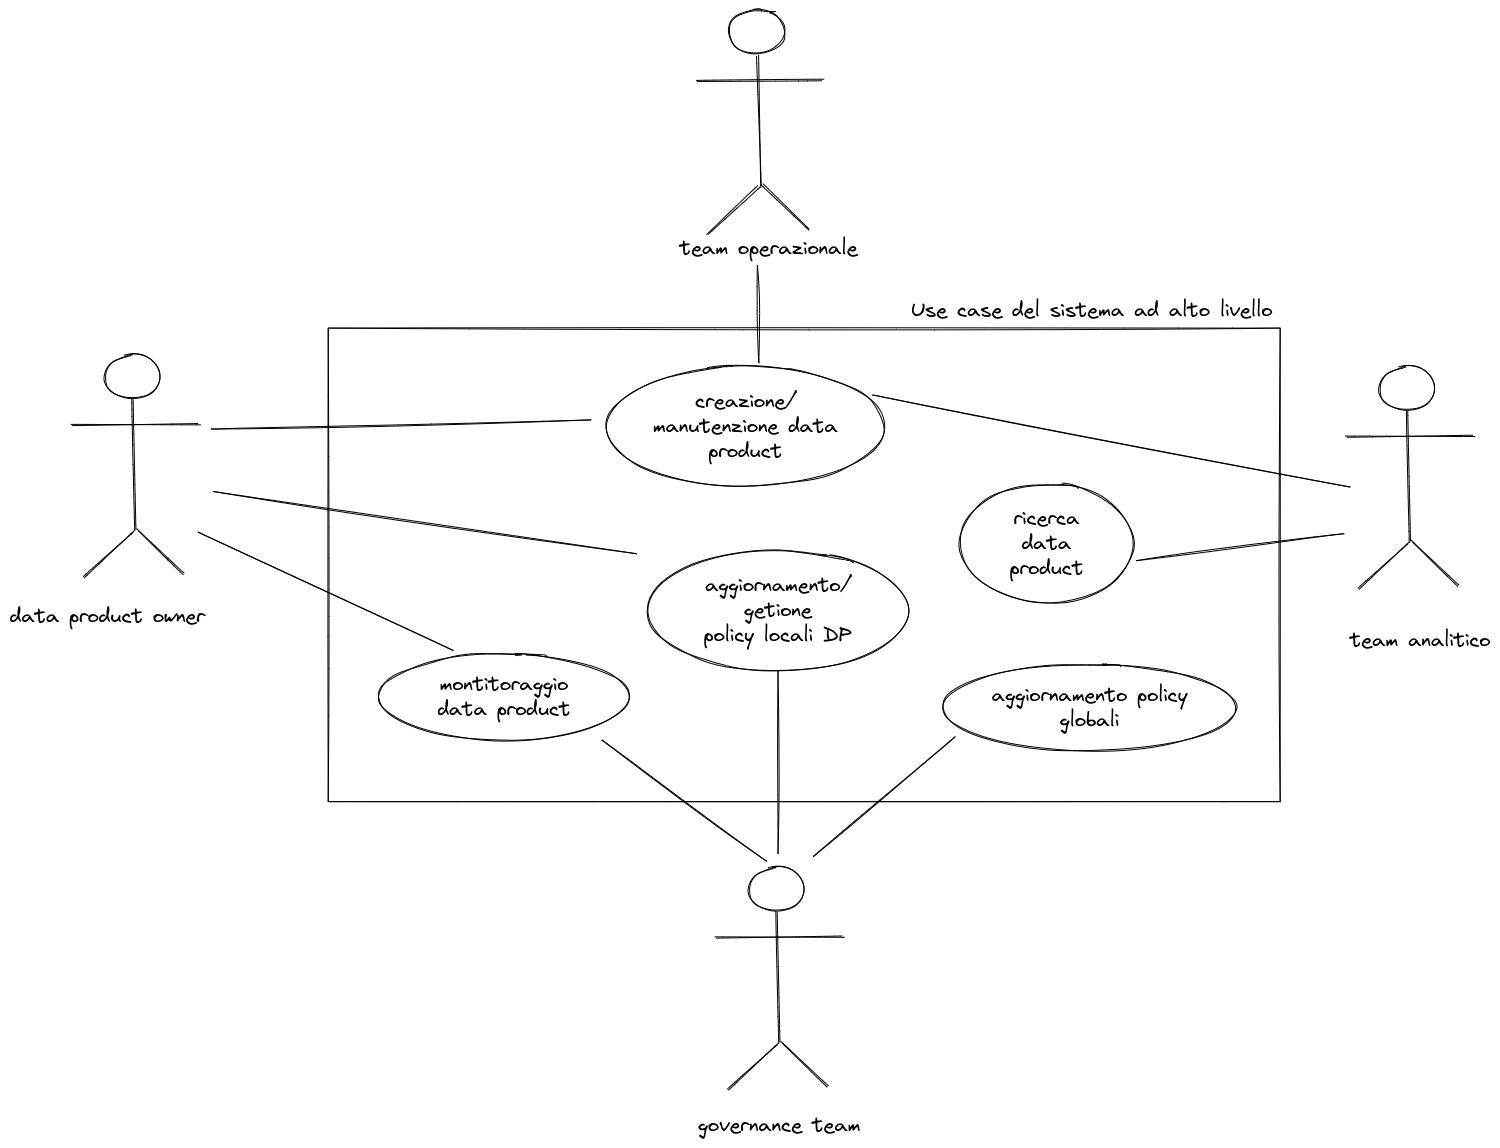
\includegraphics[width=0.75\linewidth]{immagini/business use cases data mesh SOA 2023-07-06 10.49.16.excalidraw.png}
        \caption{Sintesi dei requisiti, espressi sotto format di obbiettivi degli agenti coinvolti}
        \label{fig:requisitiBusiness}
    \end{figure}

\begin{table}
    \centering
    \begin{tabular}{|c|c|}
    \hline
        Elenco requisiti & Motivazioni\\
        \hline
        Supporto per ETL & Creazione Data Product \\
        Interfaccia uniforme & Creazione Data Product, Governance\\
        Integrazione con database per dati analitici & Creazione Data Product, Governance \\
        Aggiornamento dei Data Product  & Creazione Data Product\\
        Valutazione delle politiche & Governance \\
        Applicazione e codifica delle politiche & Governance  \\
        Monitoraggio della qualità  del Data Product & Governance \\
        Accesso ai meta-dati dei Data Product & Ricerca Data Product \\
        Mantenimento dei punti di accesso ai Data Product & Utilizzo Data Product \\
        Interfaccia per il team di Governance & Governance \\
        Sistema per il controllo degli accessi & Governance \\
    \hline
    \end{tabular}
    \caption{Raccolta dei requisiti da utilizzare per la progettazione dell'architettura}
    \label{tab:requisitiTec}
\end{table}
\section{Componenti e Responsabilità}\label{componenti e responsabilità}
In questo paragrafo  si introducono le componenti ritenute necessarie per la realizzazione dell'architettura.
Per spiegare la necessità delle componenti proposte per la piattaforma si è partiti considerando una Data Mesh che non ne prevedesse l'uso. 
Sono quindi stati analizzati i limiti della soluzione e iterativamente introdotte nuove componenti.
In questo paragrafo viene ri-proposto il percorso di progettazione svolto.
Le componenti sono state poi ri-organizzate in modo che rispecchino l'ordine con cui si consiglia di realizzare i vari strumenti.
In un sistema enterprise, infatti, i team analitici e i team operazionali saranno già impegnati nello svolgimento e nella manutenzione dei loro sistemi.
Si ritiene che il team assegnato alla piattaforma debba sviluppare gli strumenti in maniera graduale, chiedendo agli altri team un'integrazione progressiva nei sistemi in funzione e un feedback sul funzionamento e su eventuali modifiche.
Questo permette di poter cambiare il sistema durante la realizzazione e non a posteriori.
Si cerca quindi di ottenere un confronto costante col committente, come indicato dal manifesto Agile \cite{fowler2001agile}.
Fornire inoltre una vista sull'architettura per ogni componente permette di considerare diverse varianti, adottabili in base ai requisiti e agli sforzi che si intende dedicare alla costruzione della piattaforma.

\subsection{Data Mesh senza Self-Serve Data Platform}
La prima e più elementare forma di Data Mesh presentata, vede come unico vincolo la presenza di Data Product come servizio.
Si lascia dunque a ogni team la responsabilità di costruire e mantenere in autonomia il proprio Data Product.
Si richiede, specificando che un Data Product debba essere un servizio, che questo offra un'interfaccia, per garantire al resto dell'enterprise di utilizzare i dati analitici conservati.
\begin{figure}
    \centering
    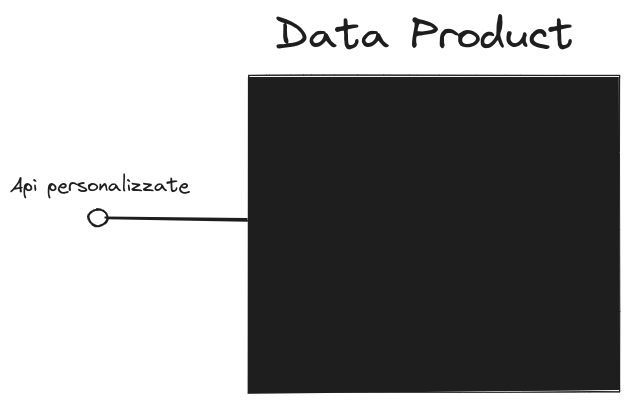
\includegraphics[width=0.5\linewidth]{immagini/data mesh elementare.png}
    \caption{Data Product senza Self-Serve Data Platform}
    \label{fig:dp senza SSDP}
\end{figure}

Viene rappresentato nella Figura \ref{fig:dp senza SSDP} come una black-box che espone un'interfaccia personalizzata.
Il vantaggio di questo tipo di soluzione è che non richiede una infrastruttura specifica e che lascia ai team la massima libertà.
Di contro non viene rispettato il principio DRY (don't repeat yourself), in quanto viene richiesto a ogni dominio di effettuare ETL, integrarsi con un database per conservare i dati analitici, creare l'interfaccia e così via.
Anche il carico di lavoro a cui sono sottoposti i team analitici e operazionali diventa importante.
La costruzione di un Data Product da zero, tenendo conto delle proprietà che un Data Product dovrebbe garantire, richiede uno sforzo non indifferente.
Per la gestione dei dati analitici in tutti i Data Product diventa inoltre la presenza di data engineer o di figure con competenze simili in ogni team.
Questo è dovuto all'alto livello di specializzazione richiesto dagli strumenti per la gestione di dati analitici nel panorama tecnologico attuale.
Sempre per lo stesso motivo queste figure sono difficili da trovare, e quindi risulta particolarmente critico e dispendioso l'inserimento di una di queste figure in ogni team.
Inoltre senza l'imposizione di un'interfaccia comune sarà necessaria la costruzione di un'integrazione ad hoc per ogni Data Product con il quale si vuole lavorare. 
Per risolvere questo problema è possibile imporre degli standard per garantire l'interoperabilità fra Data Product.
Si viene così meno al principio di Federated Computational Governance, che prevede che se possibile le scelte di Governance valide su tutti i Data Product andrebbero se possibile automatizzate. 

\subsection{Mediatore Data Product}
La prima componente che si propone per l'architettura è un mediatore per l'accesso ai Data Product.
Si propone che questo servizio venga fornito dalla Self-Serve-Data-Platform sotto forma di servizio applicativo, come riportato nella Figura \ref{fig:dp solo mediatore}.
\begin{figure}
    \centering
    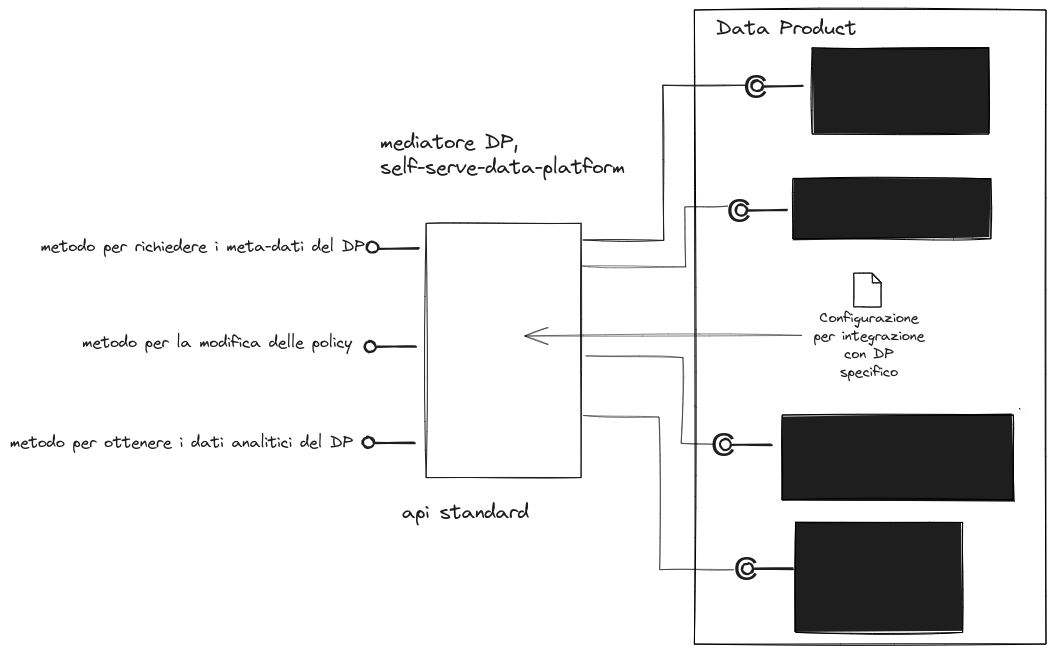
\includegraphics[width=\linewidth]{immagini/Data mesh con interfaccie.png}
    \caption{Data Mesh con mediatore}
    \label{fig:dp solo mediatore}
\end{figure}
In questo paragrafo verranno spiegate le caratteristiche che si ritengono necessarie per il servizio, si approfondiranno poi le motivazioni che hanno portato all'introduzione di questa componente nell'architettura.
La responsabilità di questa componente è fornire un'interfaccia standard a ogni Data Product.
In particolare verrà creata un'istanza del servizio per ogni Data Product.
Il Data Product si integrerà con il mediatore utilizzando un file di configurazione, o un meccanismo simile.
Nella Figura \ref{fig:dp solo mediatore}  viene mostrato il mediatore che, dato il file di configurazione mantenuto dal Data Product, si integra con altre componenti di questo, che vengono rappresentate come black-box.
È necessario che il file di configurazione contenga almeno i punti di accesso delle componenti interne al Data Product, specificando quale tipo di richiesta va inoltrata a quale componente.
Verranno qui approfondite le caratteristiche  dell'interfaccia pensata per questa componente.
Per chiarezza definiamo con metodo ogni punto di accesso che l'interfaccia espone.
Viene richiesto che il mediatore presenti un metodo per consentire l'accesso alle informazioni conservate. 
Fornire dati analitici infatti è l'obbiettivo principale di un Data Product.
Nella sua forma più semplice il metodo risponde a una richiesta fornendo i dati conservati nel Data Product.
Vengono ora proposte alcune funzionalità ulteriori che si ritiene possano essere integrate nel metodo.
Prima di tutto si potrebbe specificare tramite l'interfaccia una preferenza sulla rappresentazione dei dati. 
Un Data Product infatti secondo \cite{zhamak_dehgani_data_2023} potrebbe presentare i dati in più modi, con lo scopo di facilitarne utilizzi differenti.
Un'altra possibile aggiunta al metodo è il controllo sul ruolo dell'utente che la sta effettuando. 
Questo, insieme a un sistema di autenticazione e all'adeguato supporto nel Data Product, permetterebbe di fornire solo alcune porzioni dei dati, in base alle politiche interne stabilite dal Data Product.
Questi sono requisiti necessari nel caso il dato contenga informazioni sensibili.
Un'altra funzionalità importante per l'interfaccia di accesso ai dati è il supporto al ``Change Data Capture'', anche detto CDC \cite{eventSourcing,petrie2018streaming}.
Con CDC si intendono un'insieme di pratiche che permettono di catturare il cambiamento nel sistema.
Questo permette per esempio di ottenere aggiornamenti incrementali riguardanti i cambiamenti del dato analitico.
Si supponga di avere un Data Product \textit{B}, che viene creato a partire dai dati conservati da Data Product \textit{A}. 
Per la creazione di \textit{B} si richiedono tutti i dati conservati in \textit{A}, che poi vengono trasformati in \textit{B} a seconda delle sue esigenze.
In seguito si vuole fare in modo che il Data Product \textit{B} rimanga aggiornato rispetto ai cambiamenti di \textit{A}.
In un sistema che supporta il CDC \textit{B} manderà a \textit{A} la richiesta di aggiornamento, fornendo un'informazione aggiuntiva, che potrebbe essere per esempio la data dell'ultimo aggiornamento ricevuto da \textit{A}.
Il Data Product \textit{A} risponderà alla richiesta mandando solo le informazioni che sono cambiate a partire dalla data specificata.
Nell'interfaccia di acceso ai dati si ritiene quindi, nel caso il Data Product effettui CDC, che il richiedente possa aggiungere le informazioni che permettano di capire i dati sufficienti per l'aggiornamento del richiedente.
In questo modo si crea un unico punto di accesso, responsabile sia dell'aggiornamento che della consulta dei dati.
Infine, un ultimo requisito per questo metodo è il supporto a un meccanismo di query che permetta di selezionare solo una parte del dato conservato nel Data Product.
Questo non è esplicitamente richiesto dai requisiti individuati nella fase di raccolta ma permette di ridurre la quantità di dati trasmessi.
Il metodo per per la modifica della politiche è uno dei requisiti individuati nel paragrafo \ref{requisiti}.
L'accesso alle politiche locali da parte del team di governance permette al team di intervenire direttamente nel caso in cui si verifichino problemi riguardanti il trattamento dei dati.
Questa interfaccia dovrebbe permettere al team di governance di specificare nuove politiche, che vadano a sovrascrivere provvisoriamente quelle esistenti.
Infine il metodo per la richiesta di meta-dati viene introdotto per permettere ai team analitici di raccogliere informazioni sui Data Product.
Il metodo dovrebbe semplicemente fornire l'accesso ai meta-dati del Data Product, organizzati in modo da poter raccontare il dato conservato.
L'introduzione del mediatore come servizio rende complessivamente il sistema più complesso.
Viene proposta con l'intento di garantire in maniera automatizzata l'adozione di un'interfaccia uniforme per tutti i Data Product del sistema.
Questo rispetta il principio di Federated Computational Governance, che suggerisce quando possibile di automatizzare le scelte che garantiscano l'uniformità dei componenti del sistema.
La creazione di un mediatore semplifica anche il lavoro dei team assegnati ai Data Product:
\begin{itemize}
    \item non è necessario uno sforzo di progettazione dell'interfaccia, 
    \item rende uniforme l'integrazione con tutti i Data Product,
    \item è possibile progettarla in modo che gestisca l' autenticazione,
    \item è possibile progettarla in modo che gestisca il controllo dei parametri nelle richieste,
    \item è possibile progettarla in modo che monitori le richieste effettuate ai Data Product, garantendo un feedback al Data Product owner.
\end{itemize}

\subsection{Adapter per database analitici e operazionali}
Uno dei problemi comuni ai team operazionali e analitici nella realizzazione di un Data Product è la gestione del database in cui i dati analitici verranno conservati.
Lasciare a ogni team questo compito permette una maggiore autonomia ma richiede uno sforzo ripetute in diversi Data Product.
Ogni team dovrebbe infatti gestire l'integrazione in modo che il database sia in grado di rispondere alle richieste esposte dal mediatore.
Questo richiede essenzialmente la possibilità di scrivere e leggere dati dal database e potenzialmente supporto al CDC e a un ipotetico linguaggio di query.
L'adozione di un database specifico per team rischia di creare un problema di lock-in, sia nei confronti del fornitore della soluzione, sia nei confronti dei membri del team, che potrebbero essere gli unici a utilizzare quella tecnologia.
Inoltre difficilmente sarà possibile assistere il team fornendo linee guida o supporto nell'utilizzo del database.
Dato che le operazioni da effettuare sulla base di dati sono essenzialmente le stesse per ogni Data Product si propone come ulteriore componente dell'architettura la realizzazione di un adapter (\cite{designPatterns}), da integrare con uno o più Database analitici.
La creazione di un adapter riduce il lock-in del venditore, in quanto tutti gli utilizzatori della componenti sono legati all'interfaccia dell'adapter.
L'interfaccia sarà poi progettata dallo stesso team che ha realizzato il mediatore, che si assicurerà siano compatibili.
Infine l'adapter dovrebbe esporre un'interfaccia ad alto livello, in modo da facilitare il lavoro dei team che ci dovranno interagire.
Si propone, oltre a fissare l'interfaccia dell'adapter di togliere il database analitico dalle responsabilità del Data Product.
Il team di governance procederà a individuare un numero limitato di database analitici, disponibili per la memorizzazione dei dati di tutti i Data Product.
Verrà quindi creati degli adapter, che esporranno un'interfaccia per i Data Product e si occuperanno dell'integrazione con i database analitici.
Si è pensato di lavorare in questo modo perché le perplessità nell'utilizzo di alcune soluzioni di storage centralizzate, per esempio i Data Lake, sono legate alla difficoltà di ricerca e di interpretare dei dati. 
Dal punto di vista tecnologico invece questo tipo di soluzione è ampiamente supportata .
Si propone quindi di predisporre un numero limitato di database per il salvataggio dei dati, diminuendo la quantità di integrazione necessarie, e si utilizzano poi i Data Product come punti di accesso logico alle risorse.
Nel caso si voglia applicare il Data Mesh in un sistema enterprise che lavora già con un unico Data Lake è possibile mantenere i dati conservati lì e cambiare semplicemente le modalità di accesso ai dati analitici, che avverranno tramite richieste ai Data Product.
Quando un'utente richiede un dato quindi effettua la richiesta al mediatore, questa viene inoltrata a un servizio interno al Data Product che si occuperà di interagire con l'adapter del database analitico. 
Infine vengono ritornati all'utente i risultati.
L'interfaccia dell'Adapter sarà quindi molto semplice, e dovrà permettere a ogni Data Product di recuperare i propri dati e/o di aggiornarli.
Per supportare la possibilità di modificare ed effettuare aggiornamenti incrementali sui dati viene suggerito in \cite{zhamak_dehgani_data_2023,fowlerBitemporalNodate}
di garantire CDC tramite il concetto di Bitemporal Data.
Con Bitemporal Data si intende la pratica di associare a ogni dato due timestamp diversi. 
Il primo indica la data a cui l'informazione risale. 
Potrebbe essere per esempio la data in cui una transazione è stata effettuata.
Il secondo timestamp indica invece la data in cui il dato è stato modificato nel sistema l'ultima volta.
Questo meccanismo permette di considerare i dati come una serie di eventi consecutivi, grazie alla presenza del secondo timestamp.
Diventa quindi possibile, memorizzando questo tipo di informazione, tracciare i cambiamenti ed effettuare aggiornamenti incrementali.
Le informazioni sui Bitemporal data possono essere memorizzate anche in forma di log, senza dover cambiare la struttura delle tabelle che li conservano.
Una volta che la piattaforma fornisce gli adapter per uno o più database analitici, ogni Data Product può scegliere con quale integrarsi, in base alle preferenze sul formato di rappresentazione del dato.
Infine, visto che i dati di Data Product diversi verranno salvati nello stesso database analitico, è opportuno che l'adapter fornisca il giusto supporto per controllare gli accessi ai dati e che mantenga i dati dei diversi Data Product separati.
Viene prevista anche la creazione di un adapter per un altro tipo di database.
I Data Product alla fonte, gestiti da team operazionali devono interagire con un database operazionale.
Il processo di ETL, che di norma estrae dati da almeno un Data Product, in questo caso dovrà effettuare le richieste al database utilizzato per supportare le operazioni di business nel caso di Data Product orientati alla fonte.
Le modalità per la richiesta dei dati e per l'aggiornamento non prevedono quindi l'interazione con un altro Data Product e dunque saranno differenti.
Inoltre è possibile che vari team operazionali lavorino con database operazionali diversi. 
Per questi motivi si propone la realizzazione di un ulteriore  adapter che si integri con i database operazionali.
L'obbiettivo è permettere la realizzazione di un'interfaccia uniforme per i sistemi di ETL, a prescindere che la fonte dell'aggiornamento sia un database o un Data Product.
Si approfondiscono ora i vincoli proposti per questo adapter.
Nella progettazione dell'adapter per i database analitici è necessario tenere conto dell'interfaccia del mediatore. 
Bisogna infatti assicurarsi che sia possibile effettuare le operazioni supportate dal mediatore sul database analitico.
Le due interfacce sono quindi legate in termini di operazioni supportate.
Nei database operazionali invece, per rendere il processo di ETL uniforme a prescindere dalla fonte è necessario garantire che parte dell'interfaccia esposta dall'adapter sia uniforme con l'interfaccia esposta del mediatore, rendendo la dipendenza fra le due componenti più forte rispetto a quella fra il mediatore e l'adapter di un database analitico.
Inoltre l'adapter dovrà gestire anche le richieste che arrivano dal sistema operazionale garantendo il normale funzionamento del database.
Oltre al supporto al CDC di cui si è già discusso si richiede quindi che questo adapter presenti un'interfaccia uniforme col mediatore per quanto riguarda la richiesta di lettura dei dati; infine che l'adapter garantisca il supporto alle operazioni normalmente svolte sul database.
Si insiste particolarmente su questa standardizzazione perché la prossima componente proposta per l'architettura garantisce, assunta la realizzazione delle componenti già proposte, il supporto all'aggiornamento automatico dei Data Product.
Diversamente dalla realizzazione degli adapter per i database analitici, la realizzazione degli adapter per i database operazionali è soggetta a qualche criticità.
Nel caso siano in uso tipologie di database operazionali diverse all'interno dell'architettura, la realizzazione degli adapter diventa un'operazione gravosa e non scalabile all'aumentare del numero di team operazionali.
In questa situazione è necessario quindi richiedere che la realizzazione dell'adapter ricada sul team operazionale.
Ci si aspetta infatti che il team sia ben preparato sulla tecnologia del database, le specifiche e i requisiti sull'interfaccia che l'adapter dovrà esporre sono invece progettati a livello di architettura.
In questa situazione il team operazionale, prima di realizzare l'adapter per il database operazionale dovrebbe valutare il rapporto costi benefici.
Ai costi della costruzione dell'adapter andrebbero comparati i costi di un sistema di gestione degli aggiornamenti del dato analitico.
Nel caso i costi dell'adapter superino di molto quelli del sistema di aggiornamento, il team operazionale può gestire in autonomia l'integrazione del Data Product con il database operazionale.
Questo comporterà però poi la realizzazione di un sistema di ETL ad hoc per il Data Product, o comunque a uno sforzo per integrarsi con gli altri strumenti che verranno in seguito proposti dall'architettura.
Nella Figura \ref{fig:AdapterDB} vengono schematizzate le interfacce delle due tipologie di adapter. 

\begin{figure}
    \centering
    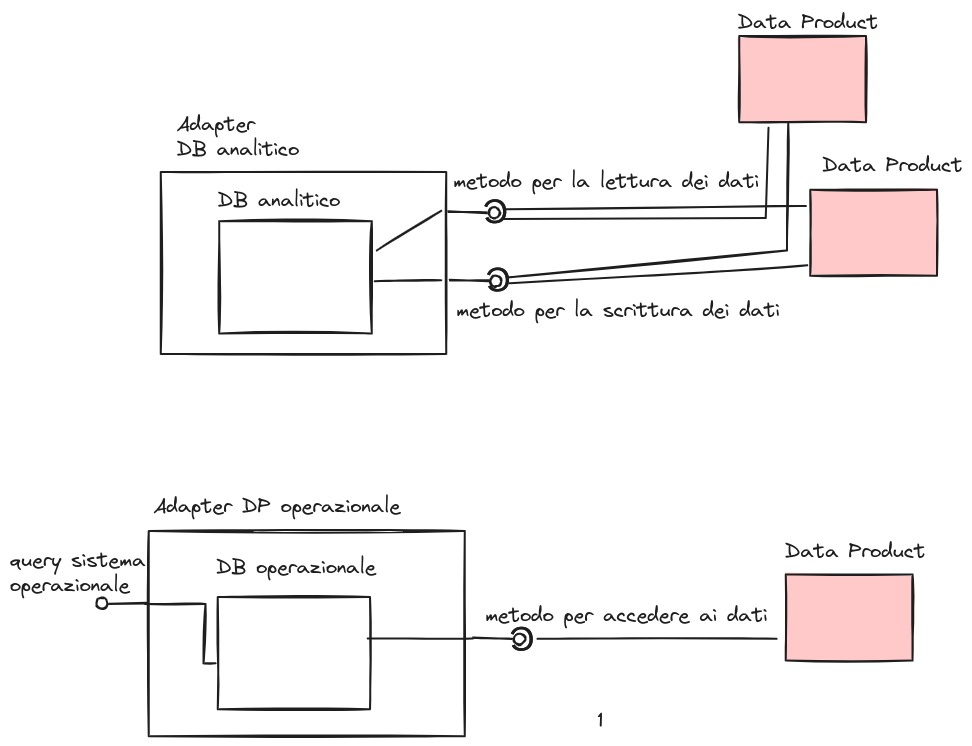
\includegraphics[width=\linewidth]{immagini/Data Mesh con DB Adapter 2024-03-06 17.45.31.excalidraw.png}
    \caption{Adapter Database analitici e operazionali}
    \label{fig:AdapterDB}
\end{figure}

\subsection{Supporto per l'aggiornamento dei dati analitici}
Come già accennato, il successivo servizio progettato per l'architettura si occupa di garantire l'aggiornamento automatico dei Data Product.
Durante la definizione del Data Product,il team responsabile dovrebbe stabilire la frequenza con cui i dati analitici debbano essere aggiornati.
Questa decisione dovrà essere svolta valutando i tipi di analisi possibili sul dato e valutando la frequenza di aggiornamento dei dati garantita dalle fonti. 
Si propone quindi un servizio, fornito dalla Self-Serve Data Platform, che utilizzi la frequenza individuata dal team per la gestione degli aggiornamenti.
Il servizio otterrà il dato analitico utilizzando il metodo di accesso ai dati che si assume essere uniforme sia nei Data Product che nei Database operazionali.
Per fare la richiesta è necessario che gli indirizzi delle fonti e il formato con cui si desiderano i dati siano comunicati al servizio.
Verrà quindi mandata una richiesta alla fonte che potrebbe richiedere una procedura di autenticazione. 
In questo caso è necessario che il servizio abbia ricevuto le credenziali o un token per l'accesso.
Per consentire gli aggiornamenti il servizio deve inoltre mantenere per ogni fonte le informazioni per richiedere solo i dati necessari all'aggiornamento, sfruttando, se presente, il supporto al CDC.
Si potrebbero, nel caso i meccanismi di query siano supportati dalle fonti, comunicare al servizio per ogni fonte il tipo di richiesta da effettuare. 
Una volta effettuate le richieste e ottenuti i dati dalle fonti, il servizio proposto dovrebbe inoltrare i dati a un altro servizio, realizzato dal Data Product per la pulizia, aggregazione e trasformazione dei dati. 
La componente che ha effettuato le trasformazioni sui dati avrà poi la responsabilità di salvarle nel Database analitico.
Chiamiamo il servizio descritto, fornito dalla Self-Serve Data Platform, gestore degli aggiornamenti.
Come per il mediatore, ogni Data Product creerà un'istanza del gestore degli aggiornamenti, passandogli un file di configurazione.
Il file, riassumendo quanto detto in precedenza dovrebbe contenere le seguenti informazioni: 
\begin{itemize}
    \item indirizzi ed eventuali query per le richieste alle varie fonti,
    \item informazioni che sfruttino l'eventuale supporto al CDC per consentire un aggiornamento incrementale,
    \item eventuali credenziali per effettuare la richiesta di dati analitici alle fonti,
    \item frequenza con cui il Data Product dovrà richiedere aggiornamenti alle fonti, 
    \item indirizzo ed eventuali informazioni aggiuntive per integrarsi col servizio che effettua aggregazioni e trasformazioni nel Data Product.
\end{itemize}
Un'altra componente opzionale potrebbe essere un servizio di notifica, che lavorerebbe in collaborazione col gestore degli aggiornamenti per informare i Data Product consumatori di eventuali modifiche alle fonti. 
Questo tipo di supporto complica leggermente il Data Product, che dovrà gestire le eventuali iscrizioni ed è da valutare nel caso ci siano Data Product che necessitano di aggiornamenti in tempo reale.
Nella Figura \ref{fig:dp supporto aggiornamenti} viene mostrata una vista su un Data Product in cui vengono precisate le componenti principali e le loro integrazioni.
In nero sono rappresentate le componenti che andrebbero implementate in autonomia da ogni Data Product in questo stadio dell'architettura.
Si è cercato di raggruppare le funzionalità e presentare un'ipotetica divisone, anche sulla base della proposta di architettura completa, che verrà sviluppata in seguito.
In bianco invece, sono mostrate le componenti fornite dalla Self-Serve Data Platform. 
\begin{figure}
    \centering
    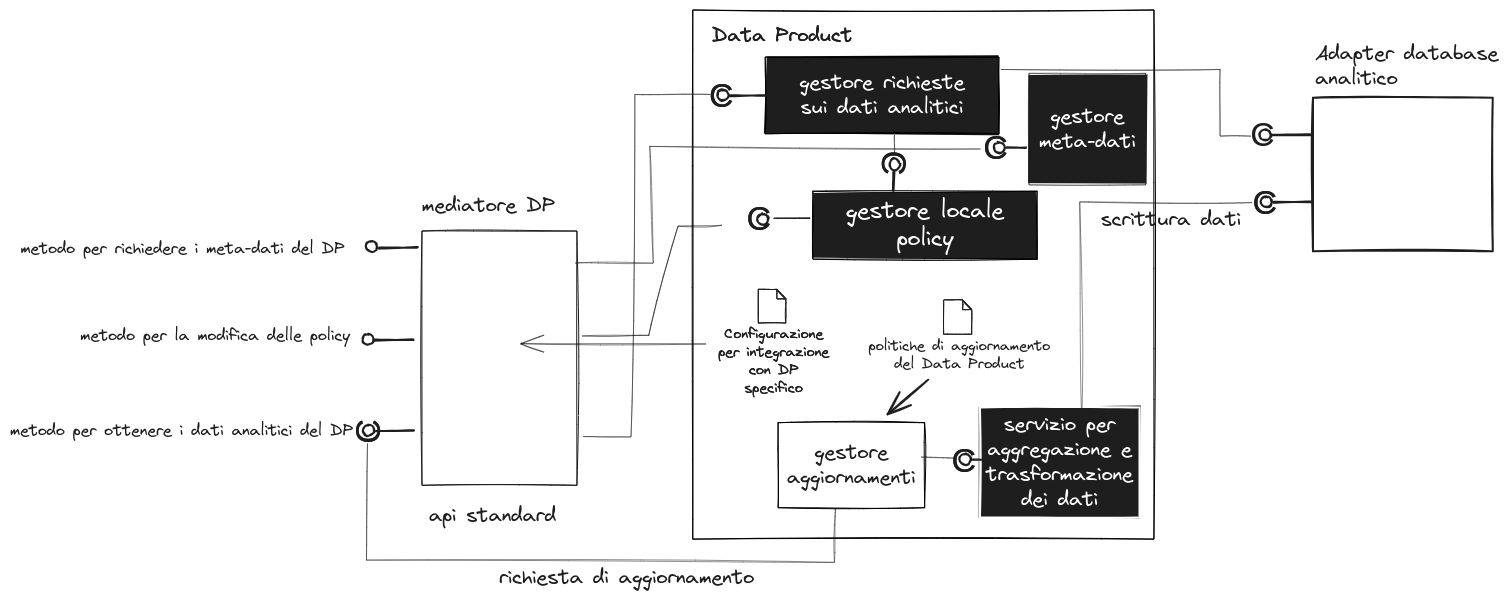
\includegraphics[width=1\linewidth]{immagini/Data Mesh supporto agli aggiornamenti 2024-03-08 15.55.58.excalidraw.png}
    \caption{Data mesh con i servizi principali definiti}
    \label{fig:dp supporto aggiornamenti}
\end{figure}

\subsection{Gestore dell'accesso ai dati analitici e delle politiche}
Quando un utente utilizza il metodo per accedere ai dati analitici del Data Product è necessario, nel caso ci siano informazioni sensibili, che vengano controllati i dati a cui l'utente ha il permesso di accedere.
Sulla base dei permessi e delle richieste dell'utente bisognerà effettuare una richiesta di lettura a un database analitico.
Dato che queste sono preoccupazioni comuni a tutti i Data Product, viene proposto un servizio con queste responsabilità.
\subsubsection{Gestore dell'accesso ai dati analitici}
Si introduce un altro servizio semplicemente per il principio di divisone delle responsabilità; le funzionalità proposte potrebbero essere integrate direttamente nel mediatore del Data Product. 
Questo servizio, che chiameremo gestore dell'accesso ai dati analitici, deve conciliare le richieste effettuate dall'utente con i vincoli fissati dalle politiche globali e locali.
Si ricorda che con politiche locali si intendono una serie di regole specifiche del dominio redatte dal team che lavora sul  Data Product, per limitare l'accesso al dato.
Con politiche globali invece si intendono le regole imposte centralmente dal team di governance e valide per ogni Data Product.
Per garantire l'automatizzazione delle politiche si è pensato di introdurre un servizio che si occupi della loro valutazione e applicazione.
Il gestore dell'accesso ai dati analitici dovrà quindi interagire con questo servizio per garantire che le politiche siano applicate.
Il servizio in questione verrà chiamato gestore delle politiche. 
Il gestore delle politiche date le informazioni sull'utente e le politiche locali e globali stabilirà le informazioni alle quali l'utente potrà accedere. 
Si ritornerà sulla definizione del gestore delle politiche a breve.
Una volta ottenute le indicazioni sulle risorse a cui l'utente può accedere, il gestore dell'accesso ai dati analitici dovrà creare una richiesta per l'adapter del database analitico.
Come già accennato in precedenza, ogni Data Product potrebbe mantenere i dati analitici in più Database analitici, per garantire rappresentazioni alternative del dato.
Nel caso venga specificata nella richiesta una preferenza di questo tipo il gestore dell'accesso ai dati analitici dovrà occuparsi di creare ed effettuare la richiesta al database analitico corretto.
Per rendere possibile l'adozione di questa componente in ogni Data Product è necessario  che le informazioni ritornate dal gestore delle politiche siano in un formato standard, e che sia definita una procedura di conversione da questo formato a quello richiesto dagli adapter.
La procedura di conversione deve essere definita per ogni tipo di database analitico supportato dall'architettura.
Infine è necessario che ogni Data Product fornisca alla componente alcune informazioni specifiche: 
\begin{itemize}
    \item endpoint degli adapter per i database analitici,
    \item endpoint del gestore delle politiche. 
\end{itemize}
Il punto di accesso a questo servizio verrà invece fornito al mediatore, che si occuperà di gestire l'autenticazione dell'utente e di trasmettere al gestore dell'accesso ai dati analitici le richieste e le informazioni dell'utente.
\subsubsection{Gestore delle politiche}
Si approfondiscono ora le specifiche del gestore delle politiche.
Come già precisato, le responsabilità del gestore delle politiche sono la valutazione e l'applicazione delle politiche globali e locali.
Per poter utilizzare un'unica componente per la valutazione delle politiche nell'enterprise è richiesto per definirle l'utilizzo di un unico linguaggio. 
Il linguaggio deve permettere la valutazione e l'applicazione automatica delle politiche dichiarate.
Le politiche locali metteranno in relazione le informazioni dell'utente con le informazioni a cui può accedere.
Le politiche globali definite dal team di governance faranno lo stesso, ma saranno valide sulle richieste di accesso a tutti i Data Product.
Per rendere effettive le politiche globali oltre al linguaggio comune è necessario che la rappresentazione delle informazioni sulla quale si vogliono stabilire politiche globali sia resa uniforme in ogni Data Product.
Si ponga per esempio che si voglia che gli utenti con il ruolo \textit{cliente} possano accedere soltanto alle informazioni associate al proprio codice fiscale.
Viene definita una politica globale che limita l'accesso agli utenti di tipo \textit{cliente} ai campi con associato un \textit{codice\_fiscale} uguale a quello del \textit{cliente}.
Per poter applicare la politiche ogni Data Product dovrà mantenere il codice fiscale utilizzando un campo \textit{codice\_fiscale}, o mantenere una procedura che associ  a \textit{codice\_fiscale} un'informazione analoga.
Richiedere uniformità in un contesto come quelle del Data Mesh è un'operazione complicata, che può portare a erosione e deriva, ma consente al team di governance di esercitare controllo su tutti i Data Product.
Sarà quindi necessario equilibrare il controllo esercitato dal team centrale con le richieste di standardizzazione del dato e con la definizione di politiche globali con la necessità di autonomia dei team operazionali e analitici.
Si propone che le politiche locali siano scritte in un artefatto mantenuto dal Data Product. 
Nella scrittura delle policy locali si dovrà tenere conto dello schema con cui i dati sono effettivamente salvati.
Infatti il gestore dell'accesso ai dati analitici utilizzerà le informazioni fornite dal gestore delle policy per effettuare le richieste ai database analitici.
Le politiche globali saranno invece mantenute centralmente dal team di governance.
Il servizio di gestione delle politiche utilizzerà per ogni Data Product l'artefatto interno al Data Product e quello fornito del team di governance per valutare le richieste di accesso ai dati.
Il servizio è responsabile di essere responsivo a eventuali cambiamenti negli artefatti.
Il team di governance potrà intervenire sulle politiche locali contattando direttamente il servizio di gestione delle politiche tramite il metodo fornito dal mediatore. 
Il metodo dovrebbe permettere al team di governance di modificare le politiche locali, questo può essere garantito consentendo per esempio la modifica dell'artefatto contente le politiche locali. 
È possibile separare ulteriormente il servizio di gestione delle politiche in due servizi distinti, uno che si occupi della valutazione delle politiche e uno che si occupi della gestione degli artefatti.
L'introduzione di queste componenti permette al team responsabile di un Data Product di concentrarsi unicamente sulla stesura delle politiche locali, rendendo automatico il resto della procedura.

\subsection{Servizio di autenticazione}
Per consentire il rispetto delle politiche di riservatezza si forniscono agli utenti solo una frazione dei dati conservati nel Data Product.
Per garantire che questo avvenga è necessario che il mediatore del Data Product verifichi l'identità dell'utente che effettua la richiesta.
Si propone quindi l'introduzione di un servizio di autenticazione, fornito dalla Self-Serve Data Platform.
Il servizio di autenticazione potrà essere utilizzato anche dagli adapter dei database per controllare la provenienza delle richieste.
Infine potrebbe essere utilizzato anche come misura di sicurezza, per assicurarsi che i servizi interni al Data Product vengano contattati unicamente dal mediatore.
Il servizio di autenticazione deve essere centralizzato per evitare conflitti o incoerenze derivanti dalla gestione delle informazioni di uno stesso utente in punti diversi.
Inoltre, la presenza di un sistema centralizzato facilita il controllo da parte del team di governance.
Quest'ultimo dovrà progettare il servizio di autenticazione in modo che, per ogni utente, siano mantenute le informazioni necessarie per la valutazione delle politiche di accesso ai dati.

\subsection{Supporto all'accesso dei meta-dati del Data Product}
Nelle SOA può diventare complicato ottenere le informazioni necessarie per contattare i vari servizi.
La soluzione tradizionale al problema prevede l'introduzione di un registro che mantenga queste informazioni. 
Si tratta di una componente centralizzata, che conserva e fornisce su richiesta informazioni e modalità per l'accesso ai servizi dell'architettura.
L'esempio più famoso è probabilmente UDDI, progettato per fornire i WSDL di diversi Web Service \cite{curbera2002unraveling}.
A questa esigenza si affianca la necessità di facilitare  la ricerca dei dati, svolta dai data scientist.
Si propone di creare quindi un servizio che mantenga tutte le informazioni necessarie per contattare i Data Product e al contempo che permetta di capire cosa venga offerto da questi.
Il servizio, che verrà chiamato registro dei Data Product, sarà utilizzabile dall'utente per cercare i dati all'interno dell'organizzazione. 
Le informazioni mostrate dal registro dovrebbero essere mantenute dai Data Product, per garantire che team che ci lavora mantenga il pieno controllo sui dati.
Il team di governance può, nel caso lo ritenga opportuno, fissare alcune metriche che dovranno essere fornite da tutti i Data Product al fine di facilitare la valutazione.
Alcune di queste metriche potrebbero essere la freschezza dei dati, la frequenza di aggiornamento, la presenza di dati sensibili e le informazioni sulla provenienza del dato.
Il team responsabile del Data Product deve assicurarsi di utilizzare tecniche di differential privacy o simili nel caso i meta-dati possano far trasparire informazioni sensibili.
Un requisito opzionale per l'architettura è fornire degli strumenti per l'applicazione automatica di queste tecniche, nel caso si ritengano necessarie in diversi Data Product
Per mantenere il pieno controllo sul dato si propone che durante la consultazione del registro questo contatti la porta di accesso ai meta-dati del Data Product.
Al fine di ottimizzare la consultazione è possibile salvare le informazioni nel registro, e utilizzare un sistema di notifiche che permetta a quest'ultimo di essere informato di eventuali cambiamenti nei meta-dati dei Data Product.
In questo caso il registro manterrà una copia dei meta-dati ed effettuerà la richiesta di accesso solo nel caso gli venga notificato un aggiornamento.
Nello scenario più semplice il Data Product mantiene solamente un artefatto contente le informazioni necessarie per contattarlo e i meta-dati.
Ogni volta che un utente cerca informazioni su un Data Product il registro le ottiene contattando il mediatore, e si occupa della presentazione all'utente.
Nel caso si preveda una grossa quantità di Data Product, il registro andrebbe progettato per facilitarne la ricerca, integrando per esempio meccanismi di ranking e ricerca semantica.
Il registro dei Data Product potrebbe essere utilizzato anche per raccogliere metriche sull'utilizzo e sulla soddisfazione dei clienti di uno specifico dato.
Questo permetterebbe di fornire un feedback al Data Product Owner e al team di governance sull'andamento di un Data Product.

\subsection{Servizio di trasformazione e aggregazione dei dati}
L'ultimo elemento necessario per soddisfare i requisiti richiesti dall'architettura è un servizio che effettui aggregazioni e trasformazioni sui dati.
Dopo che il gestore degli aggiornamenti ha ottenuto dati dalle fonti è necessario che questi vengano salvati nei database analitici.
Questa operazione può diventare piuttosto complessa.
La rappresentazione dei dati ricevuti potrebbe essere diversa da quella che si vuole mantenere nel database analitico; inoltre anche i dati ricevuti provenienti da fonti diverse potrebbero essere rappresentati diversamente.
I dati provenienti da fonti diverse potrebbero essere aggiornati con frequenze differenti, e questo rende difficile la loro aggregazione, soprattutto se il criterio scelto per l'aggregazione è di tipo temporale.
Infine alcuni dati ricevuti potrebbero essere considerati non rilevanti per gli scopi del Data Product, e di conseguenza dovranno essere rimossi.
Il team con la responsabilità di realizzare il Data Product dovrà decidere e codificare i criteri per l'aggregazione e la trasformazione dei dati.
Si propone che la piattaforma fornisca un servizio che supporti queste operazioni, con l'obbiettivo di facilitare la codifica e l'esecuzione delle trasformazioni richieste.
In particolare, il servizio dovrà garantire una flessibilità sufficiente per permettere al team di effettuare operazioni specifiche rispetto al dato conservato.
Inoltre dovrà integrarsi correttamente con il servizio di aggiornamento, che fornirà i dati grezzi, e con l'interfaccia esposta dagli adapter dei database analitici, che salveranno le informazioni elaborate.
La suddivisione in servizi proposta è solo una di quelle possibili. 
Un'altra possibilità potrebbe prevedere un unico servizio con le responsabilità del gestore degli aggiornamenti e della  trasformazione e aggregazione del dato, e che si occupi quindi di effettuare l'intero processo di ETL.
Si è mantenuto questo servizio come ultimo tra quelli non opzionali forniti dall'architettura in quanto si ritiene che questa sia l'operazione più difficile da generalizzare.
Infatti le operazioni di trasformazione e di aggregazione del dato sono specifiche del dominio e potrebbero variare molto nei diversi Data Product.
Nella pratica quello che probabilmente garantirà la piattaforma è l'adozione di una tecnologia pensata per effettuare ETL, fornendo un supporto per alcune operazioni e l'integrazione con le altre componenti.
Questo avrà un impatto marginale sul team associato al Data Product, che avrà comunque il compito di imparare a utilizzare la tecnologia specifica e utilizzarla per definire le trasformazioni necessarie.

\subsection{Enterprise Service Bus}
Si propone come componente opzionale l'adozione di un Enterprise Service Bus.
Nell'architettura proposta non viene gestita la possibilità di modificare l'indirizzo del mediatore di un Data Product o di replicare in maniera trasparente le istanze di alcuni servizi.
Inoltre non viene proposto un meccanismo di sicurezza e/o di autenticazione che non preveda l'integrazione esplicita delle parti con il servizio di autenticazione.
Si propone quindi come componente opzionale l'adozione di un ESB per facilitare la comunicazione tra le componenti dell'architettura.
Questo porterà allo spostamento di alcune responsabilità dal mediatore alla nuova componente.
L'ESB si occuperà di instradare le richieste ai servizi corretti, di gestire l'autenticazione dietro a ogni richiesta e  eventualmente di raccogliere metriche sull'utilizzo dei vari servizi.
L'ESB potrebbe anche essere usato per effettuare controlli sui parametri delle richieste.
Come già accennato potrebbe permettere anche la replicazione e la modifica degli indirizzi fisici, che coinvolgerebbe solo l'ESB e non tutti gli utilizzatori.
La differenza principale fra l'utilizzo del mediatore rispetto all'ESB è che mentre il mediatore gestisce unicamente l'accesso al Data Product, l'ESB può essere utilizzato per facilitare la comunicazione tra tutti i servizi previsti dall'architettura.

\subsection{Servizio per la creazione di un Data Product}
Come ultimo servizio opzionale si propone un servizio che permetta la creazione automatica di un Data Product.
Fino ad ora sono stati individuati i componenti mostrati nella Figura \ref{fig:architettura completa}.
\begin{figure}[H]
    \centering
    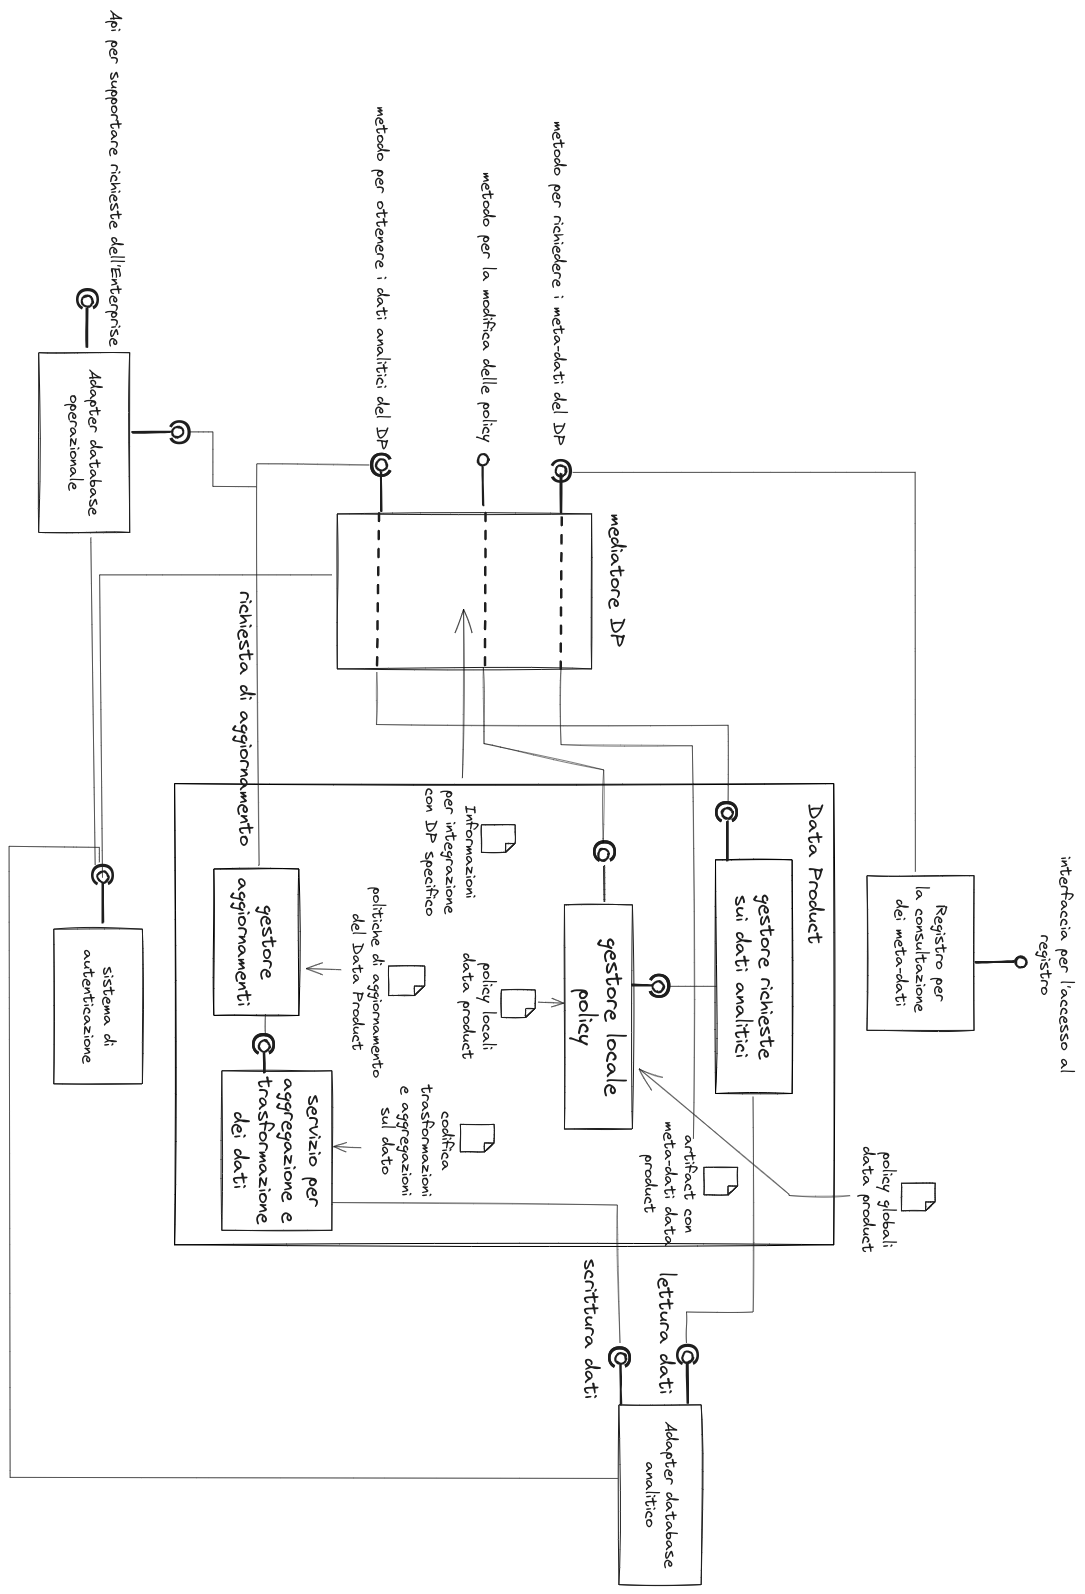
\includegraphics[width=\linewidth]{immagini/disegno completo architettura 2024-03-12 18.03.16.excalidraw.png}
    \caption{Vista completa sulle componenti proposte}
    \label{fig:architettura completa}
\end{figure}

Arrivati a questo stadio dell'architettura è possibile gestire il Data Product lavorando con gli artefatti di cui dispone.
Ogni artefatto viene passato a un servizio specifico fornito dalla piattaforma per specificare le informazioni relative al domino e gli end-point degli altri servizi con cui deve interagire.
Si propone, per concludere l'architettura, di creare una componente che data una versione ridotta degli artefatti vada a istanziare i servizi necessari per creare un Data Product.
Dato che ogni Data Product presenterà le stesse componenti e che sarà il servizio di creazione a creare le istanze degli altri servizi avrà la responsabilità di inserire negli artefatti le informazioni per l'integrazione.
La responsabilità di quest'ultima componente sarà quindi, dati gli artefatti creare il Data Product, assicurarsi eventualmente che questo sia integrato con l'ESB e che i suoi metadati siano mostrati nel registro.

\section{Osservazioni sull'architettura proposta}
Nella Figura \ref{fig:architettura completa} viene proposta una vista completa dell'architettura.
Nella rappresentazione si è cercato di mettere in risalto la divisione in componenti e le interazioni tra di esse.
Si è cercato di definire l'architettura con la minore quantità possibile di vincoli, rimanendo comunque fedeli ai requisiti individuati.
Durante la fase di analisi dei principi del Data Mesh si è giunti alla conclusione che per renderli davvero applicabili è necessario che lo sforzo per la creazione del Data Product sia minimo.
Quest'idea ha guidato tutto il processo di progettazione dell'architettura.
Si è cercato quindi di decentralizzare la responsabilità sui dati, centralizzando però lo sforzo tecnico, in quanto i team operazionali e analitici presentano anche altri obiettivi, ortogonali rispetto alla creazione del Data Product.
Questo approccio limita in parte l'autonomia dei team, ma permette di garantire un livello di controllo e di standardizzazione che altrimenti sarebbe difficile da ottenere.
Il risultato finale prevede che i team forniscano le seguenti informazioni:
\begin{itemize}
    \item le politiche locali a cui viene sottoposto il dato,
    \item le informazioni per presentare il dato al resto dell'Enterprise,
    \item i database analitici in cui il team ritiene sia opportuno mantenere i dati,
    \item le fonti e le modalità di aggiornamento del dato analitico,
    \item le operazioni di trasformazione e aggregazione da applicare ai dati ricevuti dalle fonti.
\end{itemize}
Sono responsabilità dei team la manutenzione e l'aggiornamento di queste informazioni, la realizzazione della Data Mesh viene invece delegata alla piattaforma.
Si ritiene quindi che la proposta sia in linea con il principio di Domain Ownership, in quanto i team hanno la responsabilità  e il controllo sul dato analitico.
Il registro, l'ESB, la presenza di componenti standard e la gestione interna degli artefatti facilitano la fruizione e l'autonomia, permettendo la creazione di un Data Product.
La possibilità di definire policy globali, l'accesso alle policy locali e la standardizzazione garantita dall'utilizzo delle stesso componenti all'interno dell'architettura permettono di soddisfare, dal punto di vista tecnico, il principio di Federated Computational Governance.
Infine la presenza di un'architettura per la gestione delle operazioni tecniche condivise dai domini permette di soddisfare il principio di Self-Serve Data Platform.
Nel prossimo capitolo verrà mostrato un esempio su come realizzare parte dell'architettura proposta, tramite l'implementazione e l'individuazione di tecnologie per la realizzazione di alcune delle componenti proposte.

\section{Confronto con altre architetture proposte}
In questo capitolo si è cercato di proporre un'architettura che permetta la creazione di una Data Mesh. 
Data la popolarità che l'idea di Data Mesh ha riscosso nel contesto enterprise sono state proposte diverse architetture per permetterne la realizzazione.
La maggior parte degli articoli individuati, accademici e non,forniscono esempi di architetture applicate a un contesto specifico \cite{falconi2023adopting,pakrashi2023cowmesh,joshi_data_2021,blog_data_2022}.
Il lavoro proposto si differenzia da questi in termini di obbiettivi: si è cercato di tenere un livello di astrazione maggiore, proponendo un'architettura logica indipendente dal contesto. 
Sulla stessa falsa riga sono stati individuati i tre lavori seguenti : \cite{dehghani_data_2022, majchrzak2023data,machado2021data}.
Il primo lavoro, \cite{dehghani_data_2022} definisce, oltre ai principi del data mesh, alcune linee guida e pattern per la creazione di un'architettura logica.
Si tratta del libro che ha definito l'idea di Data Mesh, ed è il riferimento principale per la definizione dei principi e per la creazione delle architetture presenti in letteratura.
In questo capitolo si è cercato, rispetto al lavoro proposto nel libro, di entrare maggiormente nei dettagli proponendo uno stile da adottare, una divisione in componenti e le loro connessioni.
Si è rimasti invece abbastanza fedeli alle proposte e ai pattern definiti nel libro.
Il secondo lavoro, \cite{majchrzak2023data}, è sempre un libro, e si pone l'obbiettivo di facilitare l'adozione dei principi del Data Mesh in un'organizzazione enterprise.
Il libro lavora principalmente in termini di processi e propone, attraverso diversi esempi, strategie per la realizzazione di una Data Mesh.
Nella parte finale vengono proposte alcune architetture, utilizzando tecnologie specifiche e concentrandosi sulla realizzazione di un ''Minimum Viable Product``.
A differenza dell'approccio adottato in questo capitolo, il libro si focalizza sull'applicazione pratica e le proposte di architettura vengono presentate solo tramite esempi.
Il terzo lavoro, \cite{machado2021data}, è un articolo che definisce un'architettura concettuale per la creazione di una Data Mesh.
Si tratta del lavoro più simile a quello proposto in questo capitolo.
L'articolo, partendo dalla mancanza di altre proposte di questo genere e dato che il libro \cite{dehghani_data_2022} rimane a un livello di astrazione molto alto, cerca di porre le basi per la creazione di un'architettura concettuale per la creazione di una Data Mesh.
Nel lavoro si parte da un'analisi del domino in cui opera una Data Mesh e si crea un modello per rappresentarlo.
Partendo dal modello si propone poi un'architettura concettuale formata da 4 parti: meccanismi di sicurezza, nodi e cataloghi, Self-serve Data Platform e infrastrutture.
Vengono poi argomentate brevemente le relazioni tra queste quattro parti. 
I meccanismi di sicurezza, che si dividono in autenticazione e autorizzazione devono essere applicati a tutti i nodi. 
I nodi sono tra loro legati da relazioni produttore-consumatore e possono essere raggiunti tramite un catalogo. 
Ogni nodo può utilizzare gli strumenti forniti dalla Self-serve Data Platform; vengono inoltre specificati i compiti che gli strumenti dovrebbero permettere di svolgere.
Infine, la piattaforma fa uso di alcune infrastrutture che devono essere garantite per il funzionamento dell'architettura.
In un lavoro uscito in seguito \cite{araujo2022advancing} l'autore propone diverse tecnologie per la realizzazione della sua architettura.
In questi due lavori non viene approfondita la struttura dei Data Product (nodi). 
Inoltre rimangono molto sintetici nella descrizione delle componenti e del loro razionale.
Il lavoro proposto in questa tesi si differenzia dall'approccio di progettazione presentato qui e in parte da quello presentato dal libro \cite{dehghani_data_2022}.
In \cite{dehghani_data_2022} si propone che la Self-serve Data Platform venga realizzata come architettura a strati; uno strato per garantire l'esperienza di utilizzo della Data Mesh nel complesso, uno strato che contenga i servizi per lavorare col Data Product e uno strato che si occupi di mediare l'accesso alle risorse computazionali o di storage.
Il lavoro proposto invece, pur creando di fatto degli strumenti che lavorano nei tre strati, organizza la progettazione partendo dal Data Product. 
Contrariamente agli altri lavori non si pone quindi enfasi sulle tipologie di strumenti da fornire ma su come questi debbano essere integrati, all'interno di un Data Product, per permetterne la realizzazione.
Si ritiene che questo tipo di approccio faciliti la standardizzazione dei Data Product che, al posto di condividere lo stesso insieme di strumenti, condividono la stessa architettura.
Le problematiche che possono emergere sono una riduzione dell'autonomia dei Data Product, che sono più vincolati da quanto proposto dalla piattaforma e si occupano unicamente di fornire ai servizi proposti le informazioni specifiche sul dominio. 
Questo aumenta la velocità di creazione di un Data Product, ma potrebbe ridurre la flessibilità e la possibilità di personalizzazione.
Visto però che il Data Product è di fatto un orchestratore di servizi è possibile che il team responsabile realizzi servizi a uso interno e li utilizzi al posto di alcuni di quelli forniti dalla piattaforma.
Questo tipo di approccio infine pone più pressione sulla piattaforma, che rischia di diventare un collo di bottiglia per l'intera organizzazione.


\chapter{Implementazione}\label{implementazione}
Nell'ultima parte del lavoro si è deciso di implementare alcuni dei servizi proposti nel capitolo precedente.
Una delle principali difficoltà nella progettazione di un'architettura è mantenere un livello di astrazione adeguato.
Il principio di vincolo minimo impone che l'architettura fornisca il minor numero possibile di limitazioni agli sviluppatori che dovranno curarne la realizzazione.
Provare a progettare e in seguito a implementare un'architettura permette di capire se i vincoli individuati sono sufficienti per definire le componenti e se l'architettura nel complesso risulta realizzabile.
Uno dei motivi per cui si è deciso di implementare alcune componenti era quindi di verificare la fattibilità di quanto proposto nel capitolo precedente.
Mostrando come sono state realizzate alcune componenti questo capitolo fornisce un esempio concreto di implementazione delle proposte fatte.
Si spera che questo processo possa anche aiutare a risolvere eventuali dubbi riguardanti le proposte del capitolo precedente.
Infine l'implementazione di alcune componenti ha permesso di mostrare alcune delle tecnologie utilizzabili per costruire l'architettura. 
Per questioni di tempo non è stato possibile realizzare l'intero sistema; ne sono state quindi selezionate solo alcune parti.
Si è deciso di seguire l'approccio proposto nel libro \cite{majchrzak2023data}, che consiglia di costruire un Data Product in maniera incrementale, partendo da un ``Minimum Viable Product'' (MVP) che garantisca semplicemente l'accesso ai dati analitici.
A differenza di quanto proposto nel libro però non si è creata un'architettura specifica per il Data Product, ma si è partiti da quanto definito nel capitolo precedente.
Nonostante la costruzione di un'architettura su misura per ogni Data Product permetta un alto livello di personalizzazione si ritiene che l'approccio possa portare a una scarsa interoperabilità, e complessivamente lo si ritiene non scalabile.
Le componenti realizzate e descritte in questo capitolo permettono l'accesso ai dati analitici attraverso la realizzazione parziale di un Data Product; sono però progettate in modo da essere facilmente riutilizzabili per crearne degli altri. 
Per semplicità si è deciso di portare come esempio l'implementazione di un Data Product fittizio.
Lo scopo del Data Product che si è deciso di sviluppare è presentare a diverse tipologie di utenti le informazioni contenute in alcune ricette mediche.
Si è deciso di lavorare simulando informazioni di questo tipo perché permettono di approfondire l'utilizzo di politiche per limitare l'accesso ai dati sensibili utilizzando il ruolo degli utenti.
Basandosi sull'architettura proposta le componenti necessarie per effettuare queste operazioni sono le seguenti: il mediatore, un adapter per l'accesso a un database analitico, il gestore delle politiche, il gestore dell'accesso ai dati analitici, ed eventualmente un ESB per facilitare la comunicazione delle altre componenti.
Nelle sezioni successive verranno presentate le tecnologie utilizzate, le caratteristiche del Data Product scelto e  verrà descritta nel dettaglio l'implementazione delle componenti e la realizzazione del sistema complessivo.

\section{Scelta delle tecnologie}
In questo paragrafo vengono spiegate le tecnologie adottate.
Si è deciso di costruire il Data Product utilizzando componenti open source per facilitare la riproduzione del lavoro.
Come linguaggio di programmazione è stato utilizzato Java, che garantisce un'integrazione semplice con le tecnologie utilizzate.
Verranno ora approfondite in ordine le tecnologie adottate per la valutazione delle politiche, il mediatore, il servizio di autenticazione e infine il database utilizzato per la conservazione dei dati analitici.

\subsection{Opa e Opal per la gestione delle politiche}\label{opa_opal}
Costruire da zero un servizio per la valutazione delle politiche può essere un'operazione complessa e dispendiosa.
In primo luogo è necessario definire un linguaggio comune, che sia abbastanza flessibile da permettere la definizione di politiche in domini diversi, ma che possa al contempo essere valutabile in automatico.
Una volta fissato il linguaggio è necessario costruire un meccanismo di valutazione delle politiche; questo deve valutare se una richiesta contente alcuni dati sia conforme con le politiche definite nel linguaggio comune. 
Il meccanismo di valutazione deve essere sviluppato, testato, mantenuto, e deve garantire un livello di sicurezza sufficiente per regolare l'accesso a dati sensibili.
Date le risorse necessarie alla realizzazione di un sistema di questo tipo si è deciso di utilizzare un servizio esistente, chiamato Open Policy Agent (OPA).
OPA è un motore di valutazione delle politiche open source\cite{noauthor_open_nodate}, che permette di definire le politiche utilizzando un linguaggio chiamato Rego.
Rego è un linguaggio ad alto livello basato su logica dichiarativa, consente di esprimere le politiche in maniera chiara e concisa.
OPA lavora con due file: un file delle politiche, in cui sono rese esplicite le regole da controllare, e un file dei dati, contente le informazioni necessarie per effettuare i controlli richiesti.
Una volta creati i due file è possibile istanziare un servizio OPA a cui vengono inviate delle richieste.
Il servizio le valuta utilizzando le politiche e i dati forniti e ritorna, sulla base di questi, una risposta.
Il formato comunemente utilizzato per la richiesta e per fornire i dati necessari alla valutazione delle politiche è il JSON.
Anche la risposta del servizio viene fornita sotto forma di JSON; questo garantisce una certa flessibilità sul tipo di richieste e di risposte che il servizio può ricevere e  fornire.
Nella Figura\ref{OPA image} viene schematizzato il funzionamento di OPA
\begin{figure}[H]
    \centering
    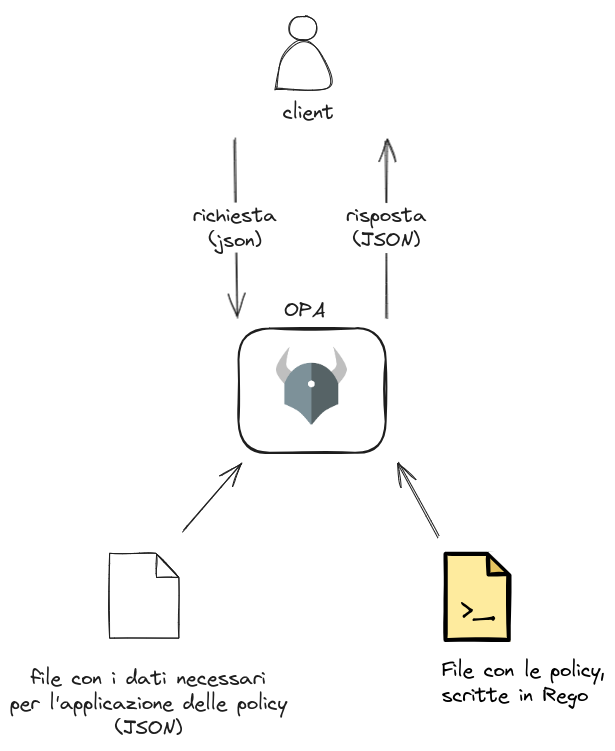
\includegraphics[width=\linewidth]{immagini/Opa funzionamento.png}
    \caption{Schema sul funzionamento ad alto livello di un servizio Open Policy Agent}
    \label{OPA image}
\end{figure}
Questo strumento fornisce il supporto necessario per realizzare il gestore delle politiche: fissa il linguaggio globale per le politiche, permette agli sviluppatori del Data Product di definire le proprie politiche locali sotto forma di artefatti e permette, date le informazioni sull'utente che effettua l'accesso, di fornire una risposta che contenga i dati a cui l'utente può accedere.

L'utilizzo di OPA per consentire la valutazione e l'esecuzione delle politiche è stato ampiamente approfondito in \cite{caronni2022framework}.
Rimangono però da soddisfare i requisiti del team di governance, che richiedono l'applicazione di politiche globali e la possibilità di modificare le politiche locali di ogni Data Product.
Per risolvere il primo problema è possibile istanziare un servizio OPA distinto che gestisca le politiche globali.
Il gestore delle politiche dovrà mandare richieste a due Open Policy Agent: quello che mantiene le politiche locali e quello che mantiene le politiche globali.
Una volta ottenute le informazioni dai due OPA dovrà creare una risposta che tenga conto della valutazione di entrambi.
Per consentire invece al team di governance di modificare le politiche locali è sufficiente fornire l'accesso al file in cui sono conservate le politiche.
È possibile aggiungere allo stack tecnologico Open Policy Administration Layer, o OPAL, per semplificare queste operazioni.
OPAL è un progetto open source che permette di aggiornare in tempo reale le politiche e i dati utilizzati da un servizio OPA.
Permette inoltre di collegare a ogni servizio più file di politiche e di dati, eliminando la necessità del gestore delle politiche di comunicare con due OPA differenti.
OPAL garantisce che un cambiamento alle politiche o ai dati, mantenute dal team centrale o dai Data Product, diventi immediatamente effettivo negli Open Policy Agent.
\begin{figure}[H]
    \centering
    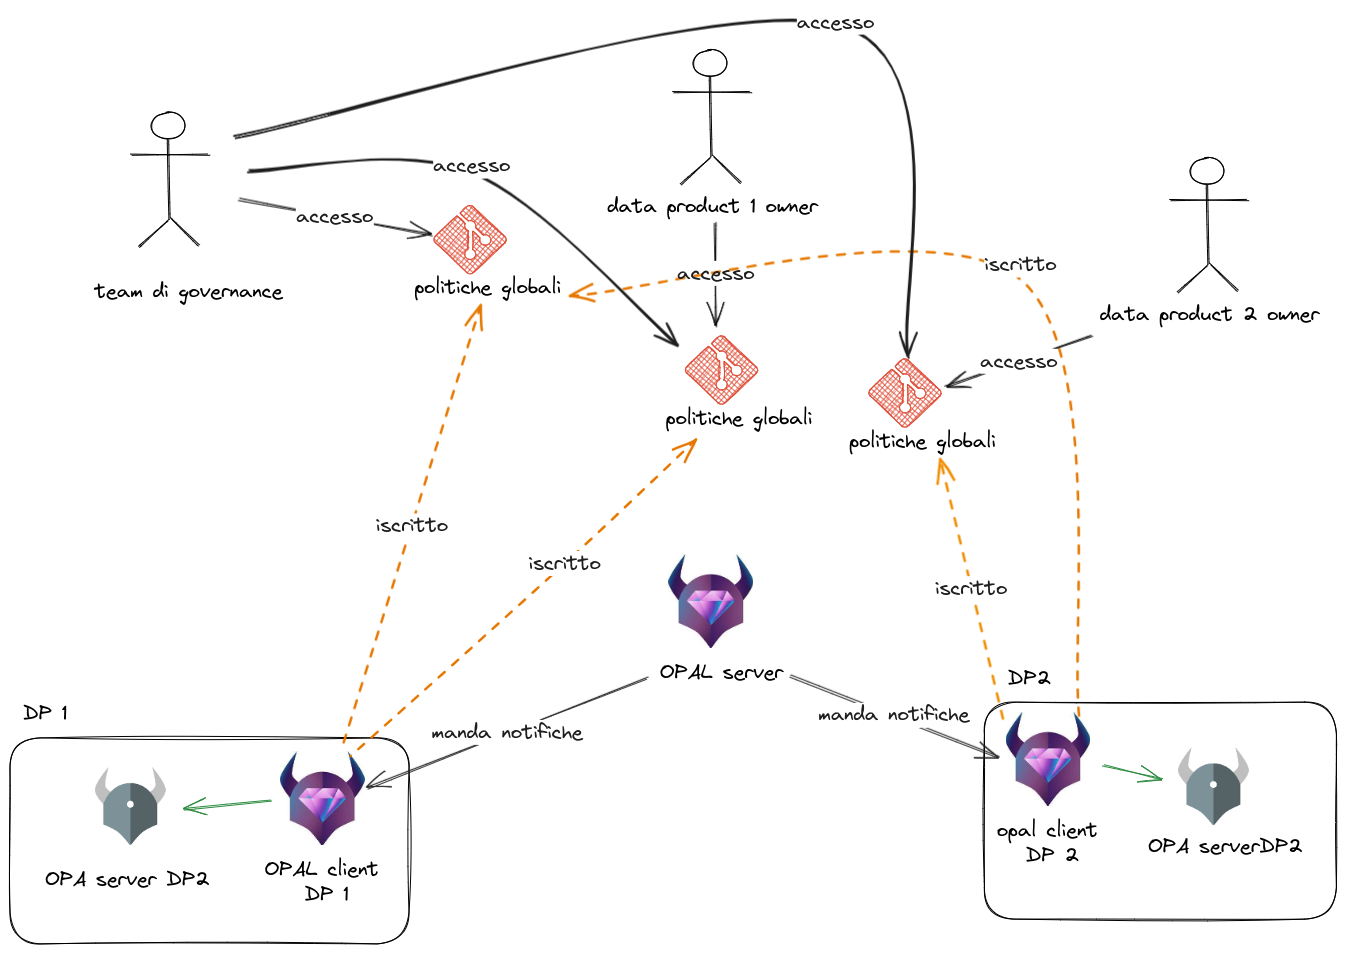
\includegraphics[width=\linewidth]{immagini/OPAL funzionamento.png}
    \caption{Schema esplicativo del funzionamento di OPAL}
    \label{funzionamento_OPAL}
\end{figure}

Si utilizza la Figura \ref{funzionamento_OPAL} per descrivere brevemente il funzionamento del servizio.
Inizialmente viene creato un server OPAL che si collega a tutte le fonti di politiche, sia locali che globali, e a tutte le fonti di dati.
La Figura mostra come il server OPAL possa per esempio sincronizzarsi con alcuni file presenti in una repository github.
Le repository che mantengono le politiche locali dovranno garantire l'accesso al file di policy al team del Data Product corrispondente e al team di governance.
OPAL implementa poi un'architettura publish-subscriber;
i server OPAL controllano le modifiche ai file a cui sono ``collegati'' e le pubblicano su alcuni ``topic''.
Ogni client OPAL si iscrive a uno o più topic e ha associato un servizio OPA.
Il client OPAL fornisce al servizio OPA i file corrispondenti ai topic a cui il client è iscritto; il servizio OPA utilizzerà questi file, che conterranno politiche o dati, per valutare le richieste.
Nel caso un file venga modificato, il server OPAL notificherà tutti i client OPAL iscritti al topic relativo a quel file; questi si occuperanno di fornite i nuovi file al servizio OPA, che potrà continuare a lavorare mantenendo le politiche aggiornate.
Per consentire la presenza di una federated computational governance, il server OPAL dovrà sincronizzarsi sui cambiamenti di tutti i file di policy e tutti i file contenti i dati necessari.
Ogni Data Product avrà un client OPAL, che si registrerà sui topic del server relativi alle politiche locali del Data Product e alle politiche globali.
Nel caso gli artefatti relativi a queste politiche venissero modificati il client OPAL si occuperà di mantenere aggiornato il servizio OPA associato.
L'utilizzo di questa tecnologia dovrebbe garantire la soddisfazione dei requisiti individuati, a livello di architettura, per quanto riguarda il gestore delle politiche.
Data la presenza di un solo Data Product nell'implementazione è stato utilizzato unicamente un servizio OPA.

\subsection{Wso2 per mediare l'accesso ai dati e fornire un servizio di autenticazione}
Quando un utente effettua una richiesta a un  Data Product è necessario che venga verificata la sua identità.
Infatti la valutazione delle politiche per l'accesso ai dati richiede le informazioni associate all'identità dell'utente.
Questo processo richiede la presenza di un servizio centralizzato che mantenga le informazioni necessarie per ogni utente e un meccanismo di autenticazione che garantisca l'accesso dopo che è stata verificata l'identità.
Per motivi di sicurezza sarebbe poi opportuno che alcuni servizi, interni al Data Product, siano accessibili solo da altri servizi.
Altre proprietà desiderabili individuate nel capitolo precedente sono la possibilità di fornire un catalogo di servizi e la possibilità di raccogliere metriche sull'utilizzo dei servizi.
Per risolvere questi problemi si è deciso di utilizzare una serie di strumenti messi a disposizione da Wso2, un'azienda che fornisce una serie di prodotti open source. 
L'obiettivo di Wso2 è permettere la creazione di architetture per sistemi enterprise in maniera veloce, facile e sicura.
Uno degli strumenti forniti da Wso2 è l'Identity Server.
L'Identity Server garantisce la gestione delle informazioni associate a ogni utente e si occupa della gestione degli accessi.
Permette quindi di registrare nuovi utenti, richiedendo e memorizzando le informazioni richieste per la valutazione delle politiche dei Data Product. 
Inoltre si occupa di verificare le credenziali degli utenti  che tentano l'accesso, e gestisce l'autenticazione utilizzando protocolli come OAuth2.
Presenta poi un complesso sistema per la gestione dei permessi, permettendo di definire ruoli e di associare a ogni ruolo determinati permessi.
L'Identity Server implementa quanto richiesto per il servizio di autenticazione, individuato in fase di progettazione.
Oltre all'Identity Server, che permette l'autenticazione, per regolare l'accesso a un Data Product è necessario utilizzare un mediatore, che si integri con il servizio di autenticazione, per gestire le richieste degli utenti.
Si utilizza un servizio di Wso2 chiamato Api Manager per l'implementazione del mediatore.
L'Api Manager permette tramite configurazioni di gestire l'accesso a un servizio specifico.
In particolare si integra con l'Identity Server per effettuare l'autenticazione, permette di esporre dei punti di accesso che vengono poi mappati su servizi interni e facilita la gestione del ciclo di vita dei servizi.
Quando un utente effettua una richiesta a un servizio, l'Api Manager contatta l'identity server per verificarne l'identità; è possibile anche fare in modo che le informazioni legate all'identità dell'utente vengano inoltrate al servizio mediato.
Il Wso2 Api Manager fornisce anche un meccanismo di controllo dei tipi nella richiesta e permette di raccogliere metriche sull'utilizzo dei servizi. 
Questa tecnologia facilita quindi la realizzazione di un mediatore che soddisfi i requisiti individuati nel capitolo precedente.
Il funzionamento del Wso2 Api Manager è schematizzato nella Figura \ref{funzionamento_api_manager}.
\begin{figure}[H]
    \centering
    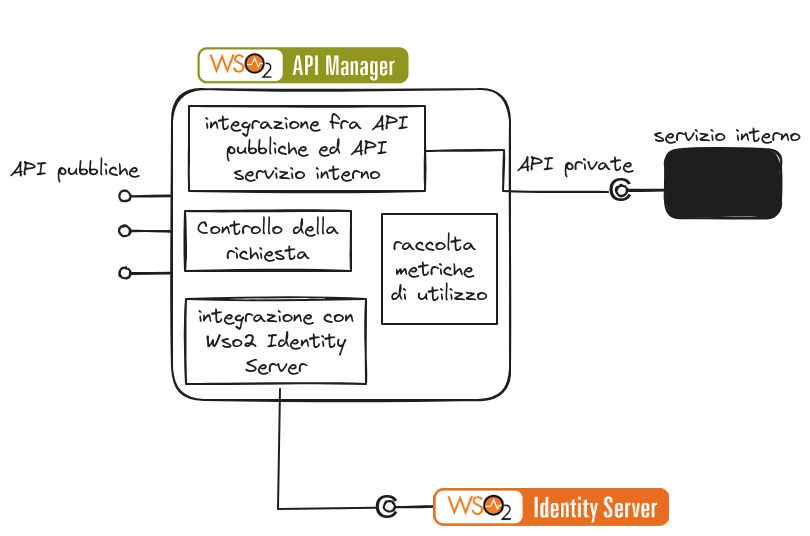
\includegraphics[width=\linewidth]{immagini/wso2 apim schema.png}
    \caption{Schema sul funzionamento del Wso2 Api Manager}
    \label{funzionamento_api_manager}
\end{figure}
Una volta appreso il funzionamento della tecnologia, a meno che non siano richieste operazioni particolari, l'API manager permette di realizzare un mediatore in pochi passaggi.
Dato che lo sforzo di creazione del mediatore tramite lo strumento è contenuto è possibile mediare l'accesso a tutti i servizi forniti dalla Self-Serve Data Platform.
Questo permette di controllare l'accesso ai servizi ``interni'' al Data Product, soddisfacendo uno dei requisiti individuati per l'ESB.
Infine, il Wso2 Api Manager crea un catalogo dei servizi che vengono mediati. 
Questo catalogo non soddisfa appieno i requisiti individuati per il registro dei Data Product, principalmente perché a differenza di alcune alternative, come DataHub \cite{datahub}, non è pensata per la presentazione di dati.
Il catalogo fornito permette però di trovare facilmente gli end-point dei vari servizi; inoltre nel caso un servizio debba cambiare l'indirizzo fisico dovrà riportare la modifica solo nella configurazione dell'API manager, mantenendo inalterata l'integrazione con gli altri componenti.
Questo, insieme al supporto fornito per il versioning dei servizi fornito dal API manager, diminuisce la resistenza al cambiamento dei servizi. 
Infine, la suite Wso2 fornisce anche uno strumento chiamato micro-integrator, che permette di specificare e gestire politiche più complesse di instradamento delle richieste.
Questo strumento non è stato utilizzato nell'implementazione, ma potrebbe essere utile per la realizzazione di un ESB.
La suite Wso2 fornisce un supporto adeguato la realizzazione di alcune componenti individuate; di contro si tratta di un prodotto complesso e non sempre intuitivo.
La community, per quanto tendenzialmente entusiasta, riporta alcune perplessità sulla documentazione, che spesso non fornisce esempi completi o aggiornati.
In una situazione reale si consiglia quindi di valutare l'adozione considerando il tempo necessario per formare il team sulla tecnologia.

\subsection{postgresql}
per il salvataggio dei dati analitici si è deciso di utilizzare postgresql.
viene definito nella documentazione del sito come segue: ``postgresql is a powerful, open source object-relational database system that uses and extends the sql language''\cite{noauthor_postgresql_nodate}.
le motivazioni per cui si è scelto di utilizzare postgresql sono le seguenti:
\begin{itemize}
    \item: postgresql è un database open source,
    \item viene utilizzato in molte applicazioni e ha un vasto supporto,
    \item è un database relazionale, che risulta più familiare a un maggior numero di sviluppatori,
    \item si integra facilmente con java, il linguaggio di programmazione utilizzato per l'implementazione.
\end{itemize}
Nell'implementazione proposta sono state utilizzate soltanto una piccola frazione delle funzionalità messe a disposizione del database.
In un'architettura reale bisognerà valutare, in base ai requisiti e alle conoscenze del team, quale o quali database utilizzare per la conservazione dei dati analitici.
Nel Data Product che verrà implementato è sufficiente che il database permetta di salvare i dati in maniera persistente e che sia possibile effettuare delle query per estrarre i dati analitici conservati. 
La gestione degli accessi, sebbene sia una feature messa a disposizione da PostgreSQL, è stata gestita dall'adapter che utilizzerà OPA; le motivazioni di questa scelta verranno discusse nella sezioni successive.
Sebbene si ritenga che PostgreSQL sia una scelta adeguata per il salvataggio di dati analitici non la si considera una tecnologia fondamentale per la definizione dell'architettura.
Verranno invece approfondite l'interfaccia e le funzionalità messe a disposizione dall'adapter, che si integrerà con il database.
\section{Descrizione del Data Product}\label{caratteristicheDP}
Come già accennato nel paragrafo \ref{implementazione} per mostrare l'implementazione delle componenti proposte si è realizzato un Data Product fittizio.
Gli obbiettivi principali individuati per una Self-serve Data Platform sono: facilitare la creazione di Data Product, facilitare la consultazione di Data Product e consentire il controllo sui Data Product a livello di governance. 
Dato che queste operazioni ruotano tutte attorno al concetto di Data Product si è deciso, per mostrare come realizzare alcuni strumenti, di crearne uno.
Il Data Product realizzato sarà quindi un pretesto per mostrare la realizzazione di alcuni servizi generali, indipendenti dal suo dominio.
Si mostrerà anche come configurare gli strumenti e come scrivere le politiche relative al dominio specifico. 
Non avendo a disposizione dati reali all'interno di un'architettura enterprise si è deciso di simulare un Data Product che permetta di accedere a delle ricette mediche. 
Si è deciso di utilizzare dati sensibili perché questo permette di approfondire l'utilizzo di politiche per garantire un'accesso differenziato al dato.
Le politiche non vengono dunque utilizzate unicamente per consentire o negare l'accesso ai dati ma per limitarne la fruizione in base al ruolo dell'utente. 
Vengono ora definiti i ruoli degli utenti che lavoreranno con il Data Product e la tipologia di dati conservati.  
A ogni ricetta si è pensato di associare le seguenti informazioni:\begin{itemize}
    \item codice identificativo della ricetta,
    \item codice fiscale del paziente,
    \item codice fiscale del medico che ha prescritto la ricetta,
    \item numero di telefono del paziente,
    \item testo della ricetta,
    \item priorità della ricetta,
    \item codice del servizio medico,
    \item data di creazione della ricetta,
    \item data di ultima modifica della ricetta nel sistema. 
\end{itemize}
La data di creazione e la data di ultima modifica vengono mantenute per applicare l'idea di Bitemporal Data.
I ruoli pensati per gli utenti sono i seguenti:
\begin{itemize}
    \item paziente, può accedere alle proprie ricette, per discriminare i dati ai quali può accedere verrà utilizzato il suo codice fiscale,
    \item medico, può accedere alle ricette che ha prescritto, anche in questo caso i dati vengono filtrati sulla base del codice fiscale,
    \item garante della privacy, può accedere a tutti i dati,
    \item data scientist, può accedere solamente alle informazioni non sensibili presenti in tutte le ricette, in particolare al codice medico della ricetta, alle date  di creazione e ultima modifica, alla priorità e al testo della ricetta.  
    \item Data Product owner, può accedere ai dati al fine di modificarli o di creare un'altro Data Product
\end{itemize}
Nella sua forma più essenziale quindi questo Data Product consente a tipologie di utenti differenti di accedere a dati riguardanti ricette mediche.
Questo è un'esempio di Data Product alla fonte, che potrebbe poi essere utilizzato da altri Data Product per effettuare analisi sui dati conservati.

\section{Descrizione delle componenti realizzate}
In questo paragrafo viene descritta la realizzazione e/o la configurazione di alcune componenti individuate nel capitolo precedente.
Si è deciso di presentare le componenti nell'ordine in cui vengono utilizzate, durante l'accesso a un Data Product.
Si inizia quindi descrivendo il mediatore e il servizio di autenticazione, poi si passa alla descrizione del gestore dell'accesso ai dati analitici, quindi al gestore delle politiche e infine all'adapter per l'accesso al database analitico.
La descrizione di alcune componenti non sarà perfettamente aderente a quanto descritto nel capitolo precedente; questo è dovuto al fatto che la realizzazione delle stesse ha portato a riflettere sull'architettura e modificarne alcune parti.

\subsection{Mediatore e servizio di autenticazione}
Come già accennato nel paragrafo sulle tecnologie si è utilizzata la suite Wso2 per la realizzazione del mediatore e del servizio di autenticazione.
Il mediatore è stato realizzato utilizzando il Wso2 Api Manager, che permette di mediare l'accesso ai servizi.
In particolare sono stati creati due tipi di mediatori: uno per l'accesso al Data Product e uno per l'accesso ai servizi interni.
Il mediatore per il Data Product si occuperà di inoltrare al gestore dell'accesso ai dati analitici una richiesta di lettura dei dati effettuata da un utente.
Wso2 Api Manager permette di definire l'API da esporre all'utente, e come mappare la richiesta corrispondente sul servizio interno. 
Nel lavoro di tesi sono state utilizzate delle Web Api, cercando di aderire all'architettura REST.
La richiesta esposta dall'Api Manager è una GET, che come parametro opzionale permette di inserire le informazioni necessarie per effettuare un aggiornamento incrementale.
L'API manager controllerà che la richiesta contenga un token di autenticazione e contatterà l'identity server per verificarne la validità.
Infine l'API manager consente, se configurato correttamente, di inoltrare al servizio interno le informazioni sull'utente che ha effettuato la richiesta. 
Queste informazioni vengono definite e gestite dall'identity server, secondo lo standard OpenID.
L'identity server ha quindi il compito di inoltrare all'API manager queste informazioni e di garantire che vengano inserite dagli utenti in fase di registrazione.
Quando viene effettuata una richiesta all'identity server questo codifica e trasmette le informazioni dell'utente sotto forma di Java Web Token (JWT), \cite{jwt_documentation}, un formato che permette di comunicare informazioni e credenziali in maniera sicura.
Il diagramma di sequenza\ref{funzionamento mediatore} riassume le comunicazioni necessarie per garantire l'accesso ai dati analitici.
\begin{figure}
    \centering
    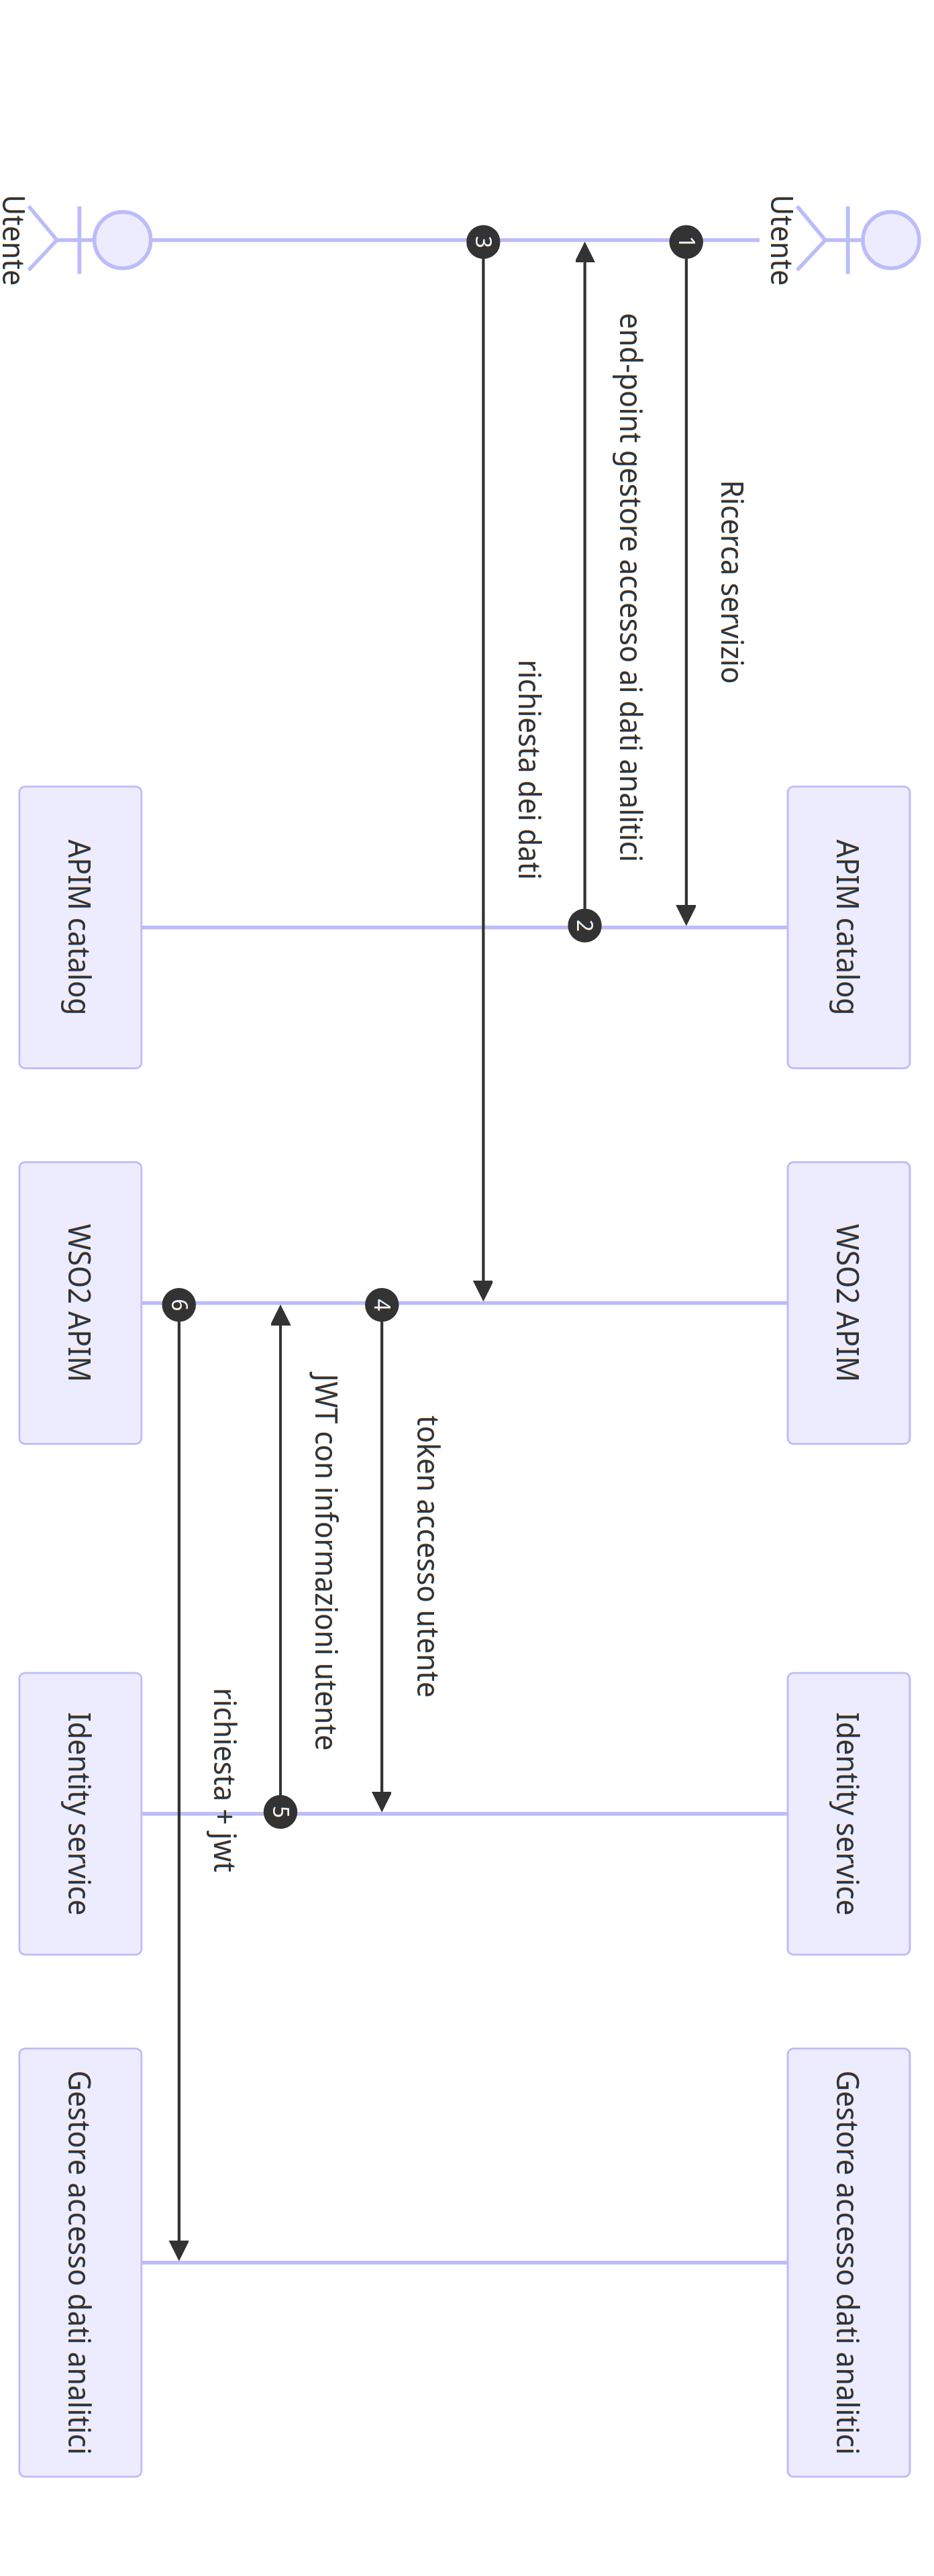
\includegraphics[width=\linewidth]{immagini/Funzionamento mediatore dati analitci.png}
    \caption{Diagramma di sequenza riguardante il le interazioni col mediatore per l'accesso ai dati analitici}
    \label{funzionamento mediatore}
\end{figure}
Il mediatore per i servizi interni funziona in maniera simile, ma possiede dei requisiti di accesso più stringenti e non richiede l'inoltro delle informazioni sull'utente al servizio.
L'API manager manderà infatti una richiesta al servizio interno solo se questa è stata effettuata da un ``utente'' con il ruolo speciale di Data Product.
Per ogni Data Product sarà creato un'utente corrispondente nell'Identity Server, e le credenziali di questo verranno utilizzate dai servizi per comunicare tra loro.
In questo modo si garantisce che i servizi interni siano accessibili solo da altri servizi.
Riassumendo sono state configurate due tipologie di mediatori che permettono di mediare l'accesso ai servizi interni e al gestore delle richieste analitiche.
E' stato poi configurato l'Identity server, creando i ruoli e le informazioni da mantenere per ogni ruolo.
Infine, sempre nell'Identity server, sono stati stabiliti quali attributi dell'utente dovessero essere inoltrati sotto forma di JWT in seguito a una richiesta.
Per effettuare quest'ultima operazione sono state ri-implementate in Java un paio di classi di Wso2.

\subsection{Gestore dell'accesso ai dati analitici}
Viene ora descritta l'implementazione del Gestore dell'accesso ai dati analitici.
L'obbiettivo del servizio è fornire dati analitici agli utenti.
Il servizio è stato realizzato utilizzando Java 11, per una maggiore compatibilità con Wso2; in aggiunta alle librerie standard sono state utilizzate le librerie riportate nella tabella \ref{tab:dependencies}.
\begin{table}[H]
\centering
\begin{tabular}{|c|c|}
    \hline
    Dipendenza & Versione \\
    \hline
    Jersey & 2.14.0 \\
    Jaxb & 2.2.4 \\
    Gson & 2.8.9 \\
    \hline
\end{tabular}
\caption{Dipendenze in Java delle librerie utilizzate dal gestore dell'accesso ai dati analitici}
\label{tab:dependencies}
\end{table}
Le librerie servono per facilitare la creazione di una web API e per la gestione dei dati in formato JSON.
Per soddisfare la richiesta dell'utente il gestore dei dati analitici deve lavorare con altri servizi.
Le informazioni sugli end-point dei servizi con cui deve interagire sono state inserite in alcuni file di configurazione.
All'avvio del servizio vengono richieste le credenziali del Data Product owner, che effettuerà l'accesso come utente con il ruolo speciale di Data Product.
Il servizio di autenticazione, nel caso le credenziali siano corrette, ritorna un token di accesso.
Il token verrà utilizzato per effettuare tutte le richieste ai servizi interni.
Il diagramma di sequenza, illustrato nella Figura \ref{fig:sequenza dati analitici}, mostra le interazioni necessarie per fornire all'utente i dati analitici.
\begin{figure}
    \centering
    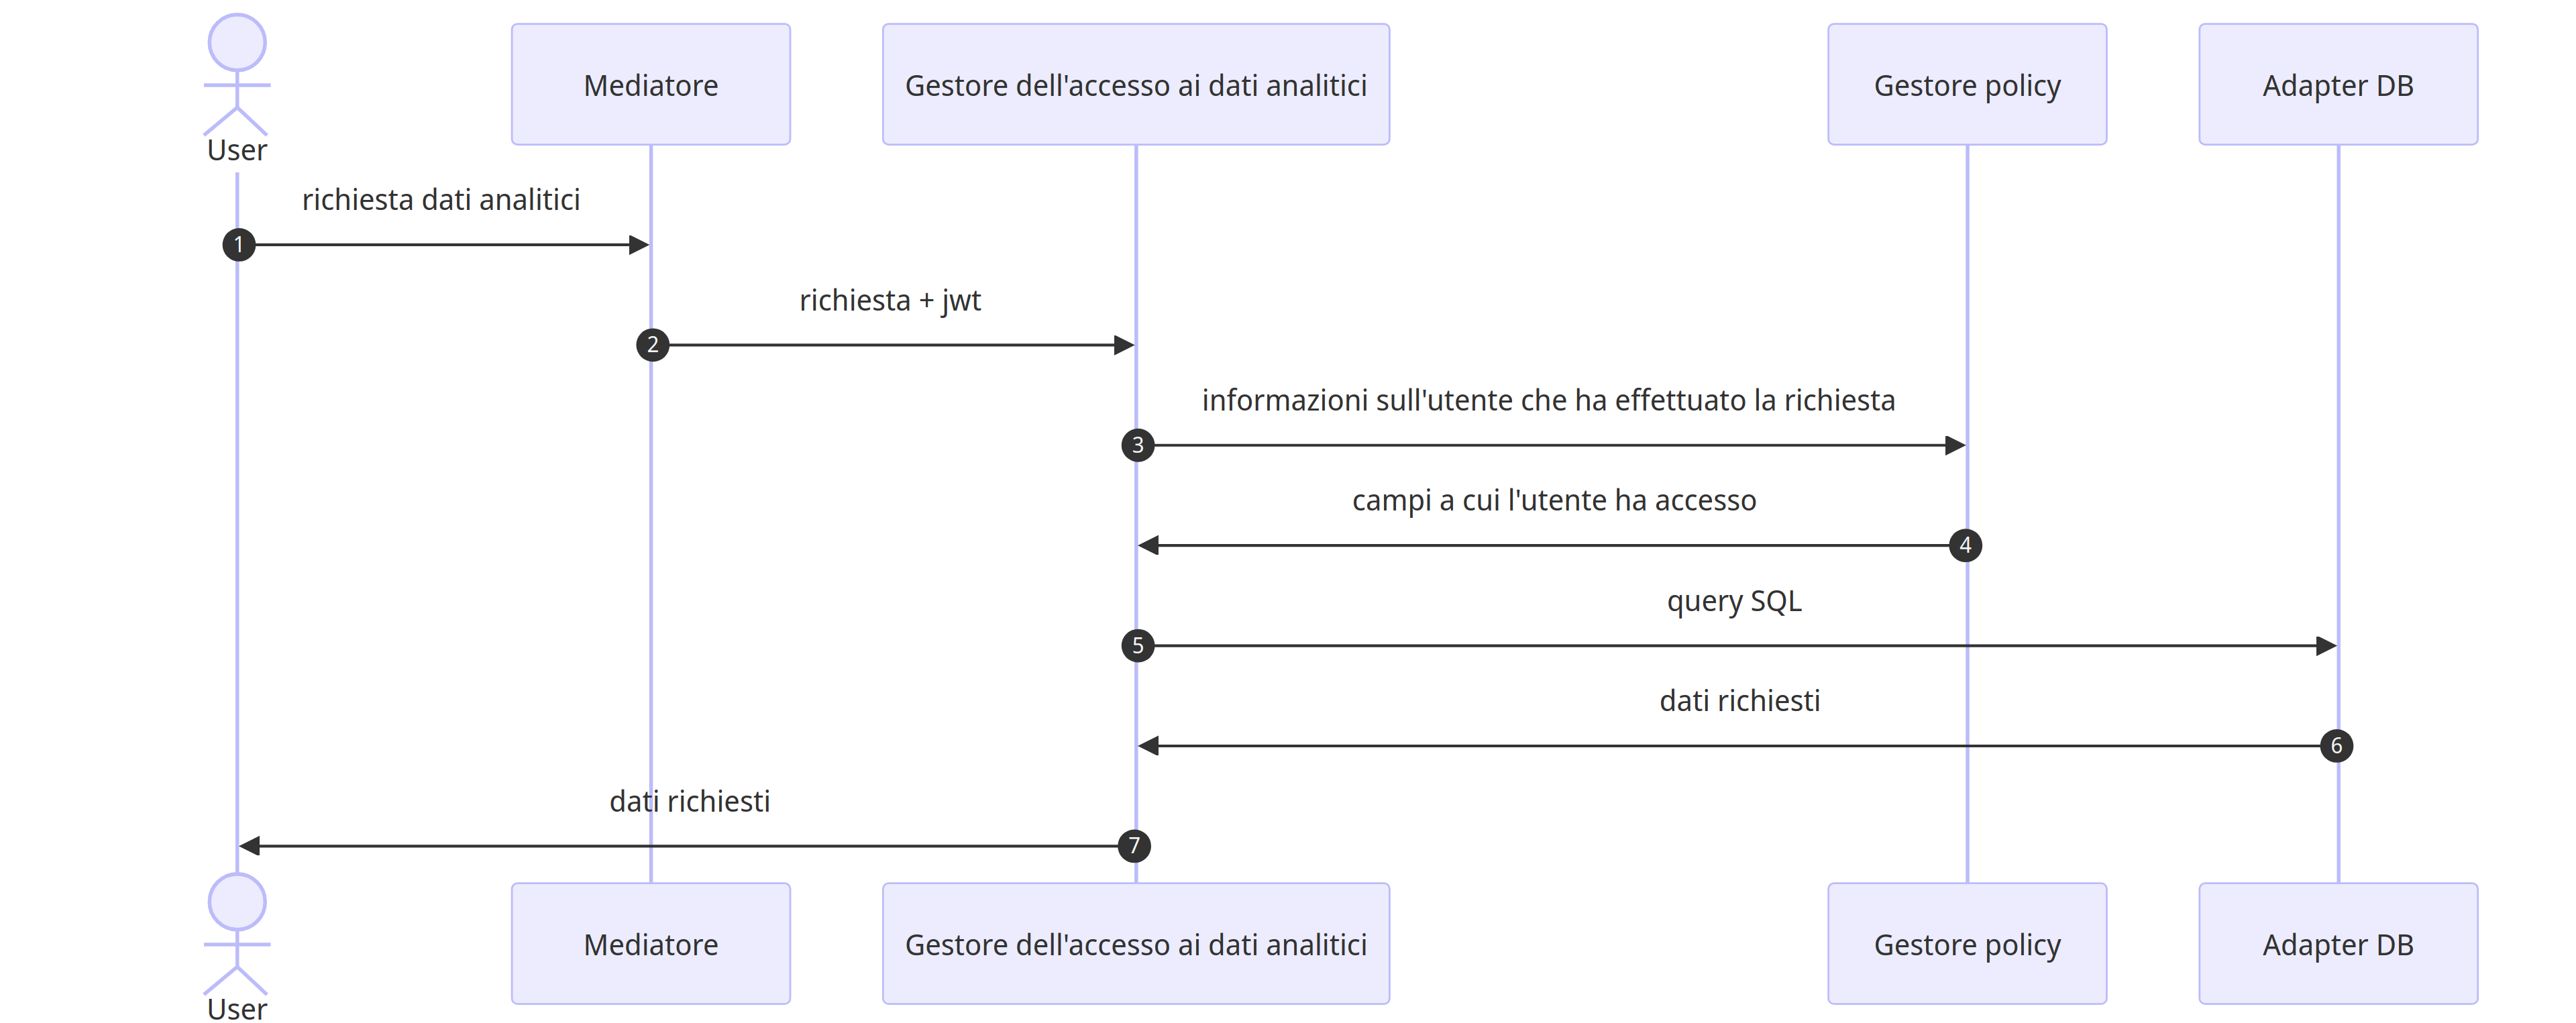
\includegraphics[width=\linewidth]{immagini/Gestore Dati analtici.png}
    \caption{Diagramma di sequenza con le interazioni necessarie per l'ottenimento di dati analitici}
    \label{fig:sequenza dati analitici}
\end{figure}
In primo luogo l'utente effettua la richiesta al mediatore. 
Le interazioni con il mediatore sono state precedentemente descritte e riassunte nell'immagine \ref{funzionamento mediatore}.
Il mediatore inoltra la richiesta al servizio, utilizzando uno dei metodi HTTP.
Il gestore dei dati analitici espone un'interfaccia molto semplice, che permette di effettuare una richiesta di tipo GET per ottenere i dati analitici.
La richiesta prevede un parametro opzionale, si tratta della data dell'ultima richiesta effettuata dall'utente, utilizzabile per richiedere solo i dati modificati successivamente alla data.
Inoltre, grazie al supporto fornito dalla libreria Jersey per la creazione di web API, l'utente potrà specificare il formato con cui preferisce ricevere i dati (JSON o XML).
Nell'header della richiesta il mediatore inserisce in forma di JWT le informazioni dell'utente che ha effettuato la richiesta.
Il gestore dei dati analitici quindi estrae dal corpo del JWT le informazioni dell'utente e le utilizza per effettuare una richiesta al gestore delle politiche.
Il gestore delle politiche risponde fornendo un elenco dei campi al cui l'utente può accedere.
Nel caso il campo non sia vuoto il gestore dell'accesso ai dati analitici dovrà effettuare una richiesta all'adapter del database analitico.
In particolare nell'esempio implementato il gestore delle politiche risponderà alla richiesta del gestore dei dati analitici con un elenco delle colonne e il nome della tabella a cui l'utente in questione può accedere.
Oltre alle colonne vengono fornite informazioni aggiuntive sulle modalità di accesso ai dati; per esempio un paziente dovrà poter accedere unicamente alle proprie ricette.
Partendo dalle informazioni sulle colonne vengono estratti gli argomenti della Select, e utilizzando le informazioni sulle condizioni vengono create le clausole Where.
Alle clausole Where viene aggiunta anche l'eventuale condizione per l'aggiornamento incrementale, fornita come parametro opzionale nella richiesta.
Sarebbe possibile inoltre estendere l'interfaccia del servizio aggiungendo come parametro opzionale la lista delle colonne a cui l'utente è effettivamente interessato.
Per creare la richiesta per l'adapter sarebbe sufficiente effettuare un'intersezione fra le colonne a cui l'utente può accedere e le colonne richieste.
Nell'implementazione della componente in un'architettura reale sarebbe opportuno fornire il supporto alla creazione di query più complesse.
Inoltre, con l'introduzione di altre tipologie di Database analitici sarà necessario permettere di specificare nella richiesta la rappresentazione dei dati desiderata ed estendere il servizio per consentire la creazione di query non SQL-based. 
Una volta creata la query questa viene inviata all'Adapter del database analitico; questo ritornerà di dati che verranno inoltrati, in formato JSON o XML all'utente.

\subsection{Gestore delle politiche}
Come già precisato nella sezione sulle tecnologie adottate per l'implementazione si è deciso che Open Policy Agent svolgerà il ruolo di gestore delle politiche.
Viene creato un servizio OPA che, data una richiesta in formato JSON contente le informazioni sull'utente, ritorna un messaggio, sempre in JSON, contenente i risultati della valutazione delle politiche.
All'avvio del servizio è necessario specificare la porta, il file con i dati e il file con le politiche scritte in Rego.
Anche questo servizio viene mediato tramite l'API manager.
Il lavoro di tesi per quanto riguarda la realizzazione di  questa componente ha comportato la creazione del mediatore tramite API manager, e la scrittura dei file contenti le politiche e i dati.
Il file con i dati contiene le informazioni necessarie a permettere l'applicazione delle politiche.
In particolare il file presenta i seguenti campi:
\begin{itemize}
    \item la lista dei ruoli a cui è permesso accedere al Data Product,
    \item le colonne presenti nel database analitico,
    \item le colonne che non contengono dati sensibili, e sono utilizzabili senza creare problemi di privacy,
    \item una mappa che associa a ogni ruolo il tipo di operazione che può eseguire sul database (lettura o scrittura).
\end{itemize}
Quest'ultimo campo è stato inserito prima di arrivare all'architettura presentata nel capitolo precedente, e nell'attuale versione nell'implementazione non viene utilizzato.
In una prima versione dell'architettura si era infatti pensato di permettere agli utenti di effettuare anche operazioni in scrittura sul Data Product e spettava quindi a OPA controllare se gli utenti avesse i permessi necessari.
In seguito si è deciso di limitare l'accesso ai dati analitici solo in lettura; le modifiche a livello di scrittura saranno a opera del gestore degli aggiornamenti, o verranno effettuate direttamente dal Data Product owner sul Database analitico.
Questo riduce il controllo sul dato ma semplifica l'architettura, migliora le performance e soprattutto aumenta la flessibilità delle operazioni di scrittura.
Le politiche dichiarate nel file Rego sono state scritte per soddisfare quanto stabilito nel paragrafo \ref{caratteristicheDP}.
La risposta fornita da OPA in seguito a una richiesta presenterà i seguenti campi:
\begin{itemize}
    \item un campo ``allow'' che contiene un booleano che indica se l'utente può accedere ai dati,
    \item un campo ``columns'', che contiene la lista delle colonne a cui l'utente può accedere,
    \item un campo ``conditions'', che contiene le condizioni che l'utente deve soddisfare per accedere ai dati,
    \item un campo ``table'', che contiene il nome della tabella a cui l'utente può accedere.
\end{itemize}
In aggiunta a questi sono presenti alcuni campi introdotti sempre per gestire le eventuali operazioni di scrittura; sono stati omessi in quanto non più utilizzati.  
Al campo ``allows'' viene assegnato il valore booleano ``true'' se il ruolo dell'utente che effettua la richiesta è tra quelli consentiti.
Il campo ``columns'' viene riempito con la lista di tutte le colonne per tutti i ruoli a eccezione del data scientist, che può accedere solo alle colonne contenti dai non sensibili.
Il campo ``conditions'' viene utilizzato solo quando gli utenti che effettuano la richiesta hanno il ruolo di paziente o di medico, e serve a segnalare che possono accedere soltanto ai record con il corrispondente codice fiscale.
%TODO : rileggo
Infine si imposta il campo ``table'', inserendo il nome della tabella in cui sono conservati i dati del Data Product.
Utilizzando queste informazioni è possibile creare una query SQL che consenta di estrarre i dati richiesti.

\subsection{Adapter per l'accesso al database analitico}
L'ultima componente implementata per l'architettura è l'adapter per l'accesso al database analitico.
Il compito dell'adapter è consentire l'accesso al database analitico, senza creare lock-in sulla tecnologia utilizzata.
Oltre a questo, data la possibilità di salvare più Data Product nello stesso database, l'adapter dovrebbe garantire una separazione dei loro dati.
L'adapter realizzato cerca di risolvere questi due problemi.
Il servizio viene realizzato tramite web API, ed è anch'esso implementato in Java.
In aggiunta alle dipendenze riportate nella tabella \ref{tab:dependencies} sono state utilizzate le librerie riportate nella tabella \ref{tab:dependencies2}, necessarie per lavorare con PostgreSQL.
Anche questo servizio viene considerato come servizio ``interno'' e viene esposto utilizzando Wso2 Api Manager.
\begin{table}
    \centering
    \begin{tabular}{|c|c|}
        \hline
        Dipendenza & Versione \\
        \hline
        PostgreSQL & 42.6.0 \\
        Ojdbc8 & 19.3.0 \\
        Jon & 3.18.6 \\
        \hline
    \end{tabular}
        \caption{dipendenze aggiuntive per l'implementazione dell'adapter del database analitico}
        \label{tab:dependencies2}
\end{table}
L'adapter espone due interfacce, una per l'accesso e una per l'inserimento o la modifica dei dati analitici.
Una volta ricevuta una richiesta è necessario assicurare che sia valida e nel caso inoltrarla al Database.
Per garantire che ogni Data Product possa lavorare soltanto sui propri dati analitici si utilizza ancora OPA.
Il servizio OPA associato al Database analitico controlla che il Data Product che effettua la richiesta stia accedendo alle tabelle a cui ha diritto.
Per garantire questa proprietà in maniera elementare nel file dei dati utilizzato dal servizio Open Policy Agent, sarà presente un campo che associa al nome di ogni Data Product una tabella del database.
L'utente, con il ruolo speciale Data Product, dovrà presentare un campo che precisa il nome del Data Product.
Le politiche del servizio verificano che la tabella associata al nome di quel Data Product sia la stessa contenuta nella richiesta effettuata.
Si è deciso di continuare a utilizzare OPA perché era una tecnologia già conosciuta e perché, essendo indipendente dal database, può essere riusata anche per altri adapter.
Inoltre il lock-in è meno rischioso, dato che si tratta di una soluzione open-source. 
Infine, come visto nel paragrafo \ref{opa_opal}, è possibile utilizzare OPAL per supportare l'aggiornamento e la gestione centralizzata delle politiche.
Nel caso la richiesta sia ritenuta valida si procede poi a effettuare la richiesta al Database e a restituire al mittente i dati richiesti.

\section{Commento dei risultati}
La parte finale del lavoro ha portato alla creazione degli strumenti per la realizzazione di un Data Product funzionante.
Il lavoro è essenzialmente un proof of concept e presenta diversi limiti.
In primo luogo l'implementazione è parziale e non fornisce quindi un'esempio concreto dell'architettura proposta nella sua interezza.
Sempre a causa della scarsità di tempo si è fatta una ricerca superficiale delle tecnologie da utilizzare e sarebbe stato interessante approfondire le alternative.
Inoltre, sebbene il Data Product proposto permetta di mostrare un esempio di accesso differenziato ai dati, il tipo di utenti e di richieste sembrano più vicine a quelle effettuate su un sistema operazionale rispetto ad un sistema analitico.
Dal punto di vista dei requisiti non funzionali sarebbe opportuno curare maggiormente la sicurezza e l'efficienza. 
Utilizzare un mediatore per ``nascondere'' gli end-point dei servizi interni infatti potrebbe creare problemi su entrambi i fronti; si è deciso di adottare questa pratica sempre a causa dei tempi limitati.
Un'altro problema importante è nella portabilità e la riproducibilità dell'ambiente. 
Infatti, sebbene la suite Wso2 sia una tecnologia open source e teoricamente portabile, risulta molto complessa e non sempre ben documentata. 
Sono sorti per esempio diversi problemi nello spostare i servizi da una macchina Windows a una macchina Linux.
Per quanto riguarda la gestione delle politiche sarebbe stato interessante provare a definire nel file .Rego una serie di politiche standard, indipendenti dal dominio.
Ogni Data Product potrebbe poi partire da queste, modificarle se necessario e utilizzare il file contente i dati per differenziasi dagli altri Data Product.
L'ultima parte su cui si sarebbe voluto dedicare più tempo è il meccanismo di conversione dei risultati dati da OPA a query SQL.
In un lavoro futuro si potrebbe approfondire la possibilità di creare policy e di conseguenza query più complesse, e provare a estendere il servizio aggiungendo il supporto per la creazione di query non SQL-based.
Nonostante queste criticità si ritiene che la realizzazione presenti alcuni spunti interessanti su come realizzare un Data Product.
Il prototipo realizzato è di fatto funzionante, utilizza tecnologie open source e i tempi di sviluppo sono stati contenuti.
I servizi realizzati sono inoltre indipendenti dal dominio e possono essere utilizzati per realizzare altri Data Product.
Le operazioni per creare un nuovo Data Product, supponendo che possa memorizzare i dati analitici una tabella SQL, sono le seguenti: 
\begin{itemize}
    \item creare file di politiche e di dati per OPA relativi al nuovo Data Product,
    \item creare dei nuovi mediatori per i servizi utilizzando WSO2 API Manager; è sufficiente partire dai mediatori già creati e cambiare gli end-point,
    \item sistemare i file di configurazione dei servizi in Java, andando a modificare gli end-point e le credenziali,
    \item creare una nuova tabella nel Database e aggiornare il file dei dati di OPA utilizzato dall'adapter per mediarne l'accesso.
\end{itemize} 
Il codice realizzato inoltre è relativamente semplice e si ritiene sia facilmente estendibile.
Si spera quindi, per quanto riguarda l'accesso differenziato ai dati e la realizzazione di Data Product con uno sforzo contenuto, che l'architettura e l'implementazione proposta possano essere d'aiuto.

\chapter*{Conclusioni}
In una parte del libro \cite{dehghani_data_2022} viene introdotto il concetto di Data Manifest, un documento che contiene le informazioni, ricavabili dal dominio, che differenziano tra loro i team con la responsabilità di fornire i dati all'organizzazione di mantenere un Data Manifest, lasciando le operazioni tecniche al team responsabile della piattaforma.
Si ritiene infatti in un contesto enterprise non tutti i team abbiano le capacità o il tempo per realizzare un Data Product, che quindi richiede il minimo sforzo possibile da parte loro.
Si è pensato che una possibile soluzione a questo problema potesse essere la realizzazione di una SOA, che definisse una serie di servizi configurabili, indipendenti dal dominio, che permettessero di realizzare un Data Product.   
\bibliographystyle{IEEEtranS} 
\bibliography{bibliography} 
\end{document}
